%==============================================================================
%  RESEARCH PAPER TEMPLATE
%  Theoretical / empirical mathematical finance
%==============================================================================
\documentclass[11pt,letterpaper]{article}

%------------------------------------------------------------------ encoding/fonts
\usepackage[T1]{fontenc}
\usepackage[utf8]{inputenc}
\usepackage{lmodern}
\usepackage{microtype}
\usepackage{textcomp}
\usepackage{eurosym}

%------------------------------------------------------------------ layout
\usepackage[margin=1in]{geometry}
\usepackage{setspace}
\onehalfspacing
\usepackage{parskip}          % paragraph spacing instead of indents (optional)
\usepackage{enumitem}
\usepackage{ragged2e}

%------------------------------------------------------------------ math
\usepackage{amsmath,amssymb,amsthm,amsfonts}
\usepackage{mathtools}        % \coloneqq, \DeclarePairedDelimiter, etc.
\usepackage{bm}               % bold math symbols

%------------------------------------------------------------------ graphics/tables
\usepackage{graphicx}
\usepackage{booktabs}         % \toprule \midrule \bottomrule
\usepackage{float}
\usepackage{caption}
\usepackage{subcaption}
\usepackage{longtable}
\graphicspath{{figures/}}

%------------------------------------------------------------------ references
\usepackage[round,authoryear]{natbib} 
\usepackage[colorlinks=true,linkcolor=blue,citecolor=blue,urlcolor=blue]{hyperref}
\usepackage{cleveref}         % \cref, \Cref, load AFTER hyperref

%==============================================================================
%  THEOREM ENVIRONMENTS
%==============================================================================
\theoremstyle{plain}
\newtheorem{theorem}{Theorem}[section]
\newtheorem{proposition}[theorem]{Proposition}
\newtheorem{lemma}[theorem]{Lemma}
\newtheorem{corollary}[theorem]{Corollary}
\newtheorem{prediction}{Prediction}[section]
\newtheorem{conjecture}[theorem]{Conjecture}

\theoremstyle{definition}
\newtheorem{definition}[theorem]{Definition}
\newtheorem{assumption}{Assumption}
\newtheorem{remark}[theorem]{Remark}
\newtheorem{example}[theorem]{Example}

%==============================================================================
%  MACROS
%==============================================================================
% --- probability / stochastic
\newcommand{\E}{\mathbb{E}}                  % expectation
\newcommand{\Prob}{\mathbb{P}}               % probability measure
\newcommand{\Qmeasure}{\mathbb{Q}}           % risk-neutral measure
\newcommand{\Var}{\operatorname{Var}}
\newcommand{\Cov}{\operatorname{Cov}}
\newcommand{\Filt}{\mathcal{F}}              % filtration / sigma-algebra
\newcommand{\given}{\,\middle|\,}
\newcommand{\Econd}[2]{\E\!\left[\,#1 \given #2\right]}  % \Econd{X}{\Filt_t}

% --- number systems
\newcommand{\R}{\mathbb{R}}
\newcommand{\N}{\mathbb{N}}
\newcommand{\Z}{\mathbb{Z}}

% --- operators
\DeclareMathOperator*{\argmin}{arg\,min}
\DeclareMathOperator*{\argmax}{arg\,max}
\DeclareMathOperator{\diag}{diag}

% --- paired delimiters
\DeclarePairedDelimiter{\abs}{\lvert}{\rvert}
\DeclarePairedDelimiter{\norm}{\lVert}{\rVert}
\DeclarePairedDelimiter{\set}{\{}{\}}

% --- shortcuts
\newcommand{\dd}{\mathrm{d}}                 % differential d
\newcommand{\eqdef}{\coloneqq}

% --- numbering
\numberwithin{equation}{section}

%==============================================================================
%  TITLE
%==============================================================================
\title{\textbf{A Structural Model of WCI Allowance Pricing}}

\author{%
  Raphael Echevin\thanks{HEC Montr\'eal and Universit\'e de Montr\'eal.
  Email: \texttt{raphael.echevin@hec.ca}.
  Financial support from the Natural Sciences and Engineering Research Council of Canada (NSERC/CRSNG) through an Undergraduate Student Research Award (USRA/BRPC) is gratefully acknowledged.}
}

\date{This version: \today}


\begin{document}
\maketitle

\begin{abstract}
\noindent
Structural models price carbon allowances as claims on the non-compliance penalty. We show this channel is inoperative in the Western Climate Initiative. The price ceiling supplies compliance instruments without quantity limit, so no firm is ever forced into default; the 4:1 untimely-surrender rule prices default at four instruments when one would have sufficed, so no firm ever chooses it. Non-compliance is thus strictly dominated and the penalty claim channel is inoperative. We instead price the allowance as a storable compliance input, solving a free-boundary problem on the allowance bank. The solution has three pricing regimes: the escalating floor, interior Hotelling growth, and marginal-abatement-cost clearing at bank exhaustion. The model's positive predictions are borne out where the data permit a test, and each doubles as a rejection of the penalty-channel alternative where that alternative makes a prediction: nine of forty-four auctions settle at exactly the reserve price, anchoring the empirical work; speculative positioning tracks the pricing regime and rejects a trend-following alternative; and the interior price--volatility relation excludes the benchmark's estimated leverage effect. A single discount wedge reconciles the model with observed price levels and moves with reauthorization news. Under the cap adopted in the 2026 California rulemaking, the bank clears by the mid-2030s in all but the steepest decline scenarios, making bank exhaustion a near-term falsifiable prediction.

\medskip
\noindent\textbf{Keywords:} cap-and-trade, carbon allowances, price floor, competitive storage, Hotelling\\
\noindent\textbf{JEL:} Q54, G12, G13.
\end{abstract}

%==============================================================================
\section{Introduction}\label{sec:intro}

In a cap-and-trade system, regulated firms surrender one allowance for each ton of greenhouse gas they emit, and a declining cap fixes the total number of allowances issued; since \citet{dales1968} and \citet{montgomery1972}, the point of the design has been that trading delivers the emissions target at minimum cost. As these systems have grown into sizable financial markets, a structural pricing literature has grown with them, and its central object is the non-compliance penalty: the allowance is valued as a claim on the penalty a firm incurs when economy-wide emissions exceed the available permits \citep{carmona2011, howison2012, hitzemann2018}. This paper shows that in the second-largest compliance carbon market in the world, that penalty is never paid, not because enforcement is lax, but because the market's own rules make paying it strictly dominated. The allowance must therefore be valued as something else, and we price it as what it is: a storable input to compliance.

The market is the Western Climate Initiative (WCI), the linked cap-and-trade system of California and Québec. The WCI shares the broad architecture of other systems: a declining cap, tradable allowances, periodic compliance. Several design features, however, distinguish it sharply from the European Union Emissions Trading System (EU ETS) that the pricing literature has in view. Banking is effectively unlimited, and the system has accumulated a large and growing bank of allowances. A regulatory floor sets a minimum auction price that escalates at five percent plus realized inflation, historically faster than the risk-free rate. A price ceiling caps the cost of compliance. Most importantly, a firm that fails to surrender enough allowances at a compliance deadline must surrender four allowances for each ton of deficit. The EU ETS, by contrast, levies a flat per-ton penalty.

A second, policy-oriented literature reaches the WCI from the other direction. It documents persistent overallocation and argues that, with the cap non-binding, only the floor creates a price incentive, so the market behaves like a carbon tax on the published reserve-price schedule \citep{cullenward2019, inman2020, vertmartin2024}. \citet{borenstein2019} predict the price will be pinned to the floor or the ceiling, and \citet{burtrawkeyes2018} document that realized prices have fallen toward the floor in essentially every emissions market. We show that the penalty view cannot hold in the WCI, and that the tax view holds exactly, but only as one regime of a larger pricing problem.

Our argument runs in three steps. First, we kill the penalty channel by dominance. The penalty is never paid for two reasons that operate in sequence. The price ceiling supplies compliance instruments without quantity limit, so no entity is ever forced into default. The 4:1 make-good rule prices default at four instruments when one would have sufficed, so no entity ever chooses it (Proposition~\ref{prop:dom}). The comparison is robust in two ways that matter later: floor and ceiling escalate at the same statutory rate, so it holds at every date; and the make-good scales with the very price a defaulter would avoid, so, unlike a flat penalty, it can never cap the price (Lemma~\ref{lem:cancel}). Never forced and never chosen: the penalty event has probability zero, and the claim that prices it is worth zero. The hard ceiling dates from 2021; over 2013--2020 dominance holds on the realized floor and interior states by the same comparison, with feasibility resting on the finite Reserve and the chronically positive bank (Proposition~\ref{prop:dom}(II)). Second, with that channel dead, the only remaining source of value is what the allowance substitutes for: holding one lets a firm avoid a future ton of abatement or a future purchase, which is exactly the logic by which storable commodities are priced. Third, we solve that storage problem. The result is a single state-constrained free-boundary problem on the non-negative bank, whose solution is the escalating floor plus a scarcity premium that switches on as the bank nears exhaustion. The solutions fall into three regimes: floor-binding, interior Hotelling, and boundary clearing. These are regions of the state space, not stages in time. The floor-binding regime recovers the policy literature's carbon-tax characterization as a special case; the other two regimes, and the transitions among them, are what the framework adds and what the WCI has exhibited since inception.

Calibrated to the price-responsive abatement supply of \citet{borenstein2019}, the framework reproduces their floor-or-ceiling conclusion endogenously, and adds what a static supply-demand analysis cannot: the bank dynamics, the regime transitions, and the sustained interior episode of 2021--2025.

\citet{working1933, working1949} and \citet{brennan1958} established that storable commodity prices reflect a complementarity between spot prices and inventory. \citet{deaton1992, deaton1996} and \citet{routledge2000} formalize this as a competitive-storage equilibrium, in which the price function has a martingale property on the interior of the stock space and a state-dependent boundary condition at the stockout point. \citet{schennach2000} first carried this structure into allowance markets, showing that banking gives the Title~IV SO$_2$ permit exactly the storage-model dynamics, with the possibility of a future stockout raising the current price. Closest to the present paper, \citet{salant2022} introduce soft price floors (auction reserve prices) into the canonical storage model and show that a floor supports the equilibrium price strictly above the floor's own level even when no auction is constrained by it---``action at a distance''; \citet{burtraw2010} anticipate the mechanism informally for price collars. \citet{salant2022} read the 2016--2017 California episode as the case in which program risk suspends that support. Our forward floor bound (Lemma~\ref{lem:floor}) is the continuous-time expression of their mechanism, and Remark~\ref{rem:2016} takes their reading of 2016--2017 as its point of departure.

Beyond the dominance result and the free-boundary formulation, three contributions follow. First, the escalator outruns the risk-free rate ($g_R>r$), which makes the floor an active obstacle. This breaks the classical variational-inequality structure and forces a decomposition of the floor carry into capacity rents and program-risk compensation, which we identify in positioning data: speculative length sits strictly inside the capacity bound throughout the chronic floor era, placing the carry on program risk. Second, a parameter-free check: nine of forty-four auctions settle at exactly the reserve price, to the cent, each in a documented episode of program-survival risk or demand collapse; the mass point certifies the discrete floor-binding regime with no calibrated parameter and anchors the regime classification on which the empirical work stands. We are explicit about what the realized sample cannot do: over an overallocated market, the substitution model and a penalty model re-parameterized to WCI conditions are close to observationally equivalent, so the sign restrictions we verify (no interior leverage effect, a flat vintage curve) are consistency checks rather than adjudication, and the behavior of positioning at transient floor touches, which is the one place the channels separate in the sample, is where the data follow the substitution reading. Third, the framework turns the legislated cap into a dated prediction: under the budgets adopted in the 2026 California rulemaking, and conditional on the calibrated short-run abatement response, the allowance bank clears by the mid-2030s in all but the steepest emissions-decline scenarios, moving the boundary-clearing regime, which is  the state in which the two channels' predictions finally diverge, from a theoretical possibility to the central determinant of the price path over the program's second decade.

The remainder of the article is organized as follows. Section~\ref{sec:model} sets out the model: the firms' emissions, abatement, and trading problem, together with the regulatory rules of the system. Section~\ref{sec:results} derives the dominance result, the substitution-based pricing equation, and the three regimes. Section~\ref{sec:calibration} takes the framework to WCI data. Section~\ref{sec:conclusion} concludes.

%==============================================================================
\section{Model Setup}\label{sec:model}
%------------------------------------------------------------------------------

We set out a stochastic equilibrium model for the WCI ETS. Table~\ref{tab:notation} collects the core notation; Appendix~\ref{app:notation} gives the complete list. The model is solved in Section~\ref{sec:results}.

\begin{table}[H]
  \centering
  \renewcommand{\arraystretch}{1.15}
  \footnotesize
  \caption{Core model notation. The superscript $i$ denotes firm $i$; omitting it
  denotes the economy-wide aggregate. The subscript $k$ indexes compliance periods.
  Time dependence is written as a subscript $t$ or in parentheses. Appendix~\ref{app:notation}
  collects the full symbol list.}
  \label{tab:notation}
  \begin{tabular}{@{}l p{0.66\textwidth}@{}}
    \toprule
    Notation & \multicolumn{1}{c}{Explanation} \\
    \midrule
    \multicolumn{2}{@{}l}{\textit{Primitives}}\\
    $\Prob,\ \Qmeasure$ & Physical and risk-neutral measures \\
    $W_t$               & Brownian motion driving aggregate BAU emissions \\
    $r$                 & Constant risk-free rate \\[4pt]
    \multicolumn{2}{@{}l}{\textit{Regulatory schedule}}\\
    $T_k,\ T$        & End of compliance period $k$; program horizon (2045) \\
    $a(t)$           & Economy-wide allocation (cap) rate \\
    $R(t),\ L(t)$    & Regulatory floor (auction reserve price); price ceiling \\
    $\Pi_t = 4S(t)$  & WCI make-good cost: $4{:}1$ untimely-surrender obligation (\S95857) \\
    $\kappa_t$       & Marginal compliance-instrument cost, $R(t)\le\kappa_t\le L(t)$ \\
    $\lambda_t,\ \ell_t$ & Risk-neutral intensity of program curtailment; fractional price loss \\
    $p$              & Risk-neutral probability of program extension past $T$ \\[4pt]
    \multicolumn{2}{@{}l}{\textit{State and prices}}\\
    $y_t$            & BAU emission rate, drift $\mu_y$ and volatility $\sigma_y$ \\
    $\xi_t$          & Abatement rate; quadratic cost coefficient $\gamma$ \\
    $\Xi(S)$         & Aggregate abatement flow, $\Xi(S)=S/\gamma$ \\
    $B_t$            & Aggregate bank of allowances \\
    $S(t)$           & Equilibrium allowance price, $S(B,y,t)$ as a function of the state \\
    $S^{\mathrm{int}}$ & Interior (Hotelling) value; $S=\max\{S^{\mathrm{int}},R\}$ \\[4pt]
    \multicolumn{2}{@{}l}{\textit{Frictions and multipliers}}\\
    $H_t,\ \bar H(t)$ & Aggregate speculative spot holdings; holding capacity (\S95920) \\
    $\eta_t$          & Shadow price of the holding-capacity constraint \\
    $\nu_t$           & Convenience yield at the stockout boundary $\{B_t=0\}$ \\
    $\tau_A$          & First time the auction is the marginal source of allowances \\
    \bottomrule
  \end{tabular}
\end{table}

An Emissions Trading System (ETS) divides time into compliance periods. At the end of each period, every firm must surrender one allowance per tonne of $\mathrm{CO}_2$ it has emitted. Firms obtain allowances from the regulator in two ways: free allowances, allocated at the start of each year at no cost, and purchases at the regulator's quarterly auctions. The regulator caps the total of allocated and auctioned allowances each year, and the cap declines over time to induce abatement.

Our setup follows \citet{hitzemann2018} closely, reusing their framework for firm business-as-usual (BAU) emissions $y_t$, cumulative emissions $x_t$, and abatement $\xi_t$.

\begin{assumption}[Emission Trading System]\label{ass:ets}
We consider an environmental market regulating a set of firms $I$ under the rules of the WCI. Compliance is organized in consecutive compliance periods partitioning $[0,T]$, period $k$ ending at the triennial surrender date $T_k$. Each firm $i\in I$ receives free allowances at the start of each year and can buy supplemental allowances at each quarterly auction. The sum of free and auctioned allowances gives the yearly cap, determined exogenously in advance.\footnote{The WCI additionally requires an annual partial surrender of 30\% of the prior year's obligation (\S95855); we model the triennial full true-up only. The simplification affects within-period flow timing but not the bank identity at the Q4 measurement points of Section~\ref{sec:data}, which read the bank after the November surrender has cleared.}
\end{assumption}

\begin{assumption}[Penalty]\label{ass:pen}
A penalty $\Pi_t$ is enforced for each missing allowance at the triennial compliance date:
\begin{equation}
\Pi_t=4S(t),
\end{equation}
so a firm short one allowance at compliance must surrender that allowance plus three penalty allowances, of which at most one can be an offset.
\end{assumption}

\begin{assumption}\label{ass:prob}
We fix a filtered probability space $(\Omega,\Filt,\{\Filt_t\}_{t\in[0,T]},\Qmeasure)$ satisfying the usual conditions, with $\{\Filt_t\}_{t\in[0,T]}$ generated by a standard Brownian motion $W_t$, the only source of randomness in the market; it represents demand and production shocks unpredictable to firm and regulator alike. Allowance prices are determined under the risk-neutral measure $\Qmeasure$. Because BAU emissions $y_t$ are not a traded asset, the market is incomplete and $\Qmeasure$ is not pinned down by no-arbitrage alone. Our baseline assumption is that emissions risk is unpriced: the drift $\mu_y$ is the same under $\Prob$ and $\Qmeasure$. This treats BAU emissions as an idiosyncratic state variable uncorrelated with aggregate consumption risk, the assumption maintained by \citet{carmona2011} and \citet{hitzemann2018} for the EU ETS. Pricing emissions risk at a market price $\lambda_y$ would add $-\lambda_y\sigma_y\partial_yS$ to the interior pricing PDE of Section~\ref{sec:results}; Section~\ref{sec:ident} bounds the contribution such a premium could make to the fitted discount wedge.
\end{assumption}

\begin{assumption}\label{ass:T}
We denote by $T$ the terminal program-end date under current legislation, at which the program either continues, possibly under a tightened cap consistent with the 2045 carbon-neutrality target, or winds down. We set the wind-down value $S^{\mathrm{wd}}(T)=0$, as allowances have no value once the market ceases to exist. We define $p$ as the risk-neutral, market-implied probability of continuation past $T$, carrying a continuation value $S^{\mathrm{ext}}(T)$ equal to the value of an allowance in the ongoing post-$T$ program. The terminal condition anchors the interior value $S^{\mathrm{int}}$ (Section~\ref{sec:interior}):
\begin{equation}\label{terminal}
S^{\mathrm{int}}(B,y,T)= p\cdot S^{\mathrm{ext}}(T) + (1-p)\cdot S^{\mathrm{wd}}(T).
\end{equation}
In the baseline we set $S^{\mathrm{ext}}(T)=R(T)$, the floor of the continuing program; solving for the continuation value as a fixed point of the framework under the post-$T$ cap is left to future work. The probability $p_t$ is not an additional risk primitive: it is a functional of the single program-survival process of Assumption~\ref{ass:jump}, whose readings at different horizons are collected below. In the empirical implementation the terminal datum is read conditional on survival, $p=1$: the survival channel is carried on the interior through the coefficient $\lambda\ell$ (Proposition~\ref{prop:intpricing}), and fitting $p$ and $\lambda\ell$ jointly would price the same survival process twice.
\end{assumption}


\begin{assumption}[Trading Activities]\label{ass:trading}
As in any ETS, emission permits are tradable OTC by compliance entities and financial speculators. We denote the spot price of the allowance at time $t$ by $S(t)$. We denote the trading strategy of firm $i$ by the adapted process $\theta^i=(\theta^i_t)_{t\in[0,T]}$, with $\theta_t^i$ the instantaneous net purchase rate of firm $i$ at time $t$ (allowances per unit time, signed: positive for purchases, negative for sales). With $c_k^i$ the free allocation given to firm $i$ for year $k$ and $\Theta^i_t=\int_0^t \theta_s^i\,ds$ firm $i$'s cumulative net position, firm $i$'s cumulative permits are
\begin{equation}
Q_t^i=\sum_{k:t_k\leq t} c_k^i+\Theta_t^i
\end{equation}
\end{assumption}

\begin{assumption}[Participants and position constraints]\label{ass:capacity}
Compliance instruments are held by two classes of participants: compliance entities and registered financial participants (``speculators''), whose aggregate spot holdings we denote $H_t$. Speculative spot positions satisfy
\begin{equation}\label{eq:capacity}
0 \leq H_t \leq \bar H(t),
\end{equation}
for a finite, exogenous capacity process $\bar H(t)$. The lower bound reflects the infeasibility of spot short sales: CITSS transfers require existing holdings and no allowance-borrowing market exists. TThe upper bound reflects per-entity holding limits, the finite registered population, and per-auction purchase limits that bound the rate of aggregate accumulation.\footnote{The holding limit is the maximum number of CA GHG allowances that may be held by an entity or jointly by a group with a direct corporate association (CCR \S95920(a), with association defined in \S95833), so it cannot be circumvented by registering affiliated entities. The per-auction purchase limit is set in \S95911(d) and aggregated across corporate associations in \S95914; bids that would breach it are rejected at clearing.}\footnote{Allowances placed in an entity's Compliance Account against accrued obligations are exempt from the holding limit under the limited exemption of CCR \S95920(d)(2)(A), so the compliance entities' problem \eqref{eq:firm-objective-finite} is unaffected by \eqref{eq:capacity}. The exemption covers current-vintage allowances; it does not extend to future vintages, which does not affect the present argument.}
\end{assumption}

\begin{assumption}\label{ass:emissions}
We characterize firm $i$'s BAU emissions as the Itô process:
\begin{equation}\label{eq:bauemissions}
y^i_t = y^i_0 + \int_0^t \mu_y^i(s)ds + \int_0^t \sigma_y^i(s)dW_s^i
\end{equation}
The stochastic term $\sigma_y^i(t)\,dW_t^i$ models unpredictable demand and production shocks. We impose a one-factor structure on the firm-level drivers, $dW_t^i=\rho_i\,dW_t+\sqrt{1-\rho_i^2}\,d\tilde W_t^i$, with the idiosyncratic components $\tilde W^i$ mutually independent and averaging out in the aggregate. Aggregate BAU emissions $y_t$ are then an It\^o process driven by the single Brownian motion $W_t$ of Assumption~\ref{ass:prob}; together with the exact cost aggregation of Appendix~\ref{subsec:hetmac}, this is what permits the equilibrium price to be a function of the aggregate state $(B,y)$ alone. A firm's cumulative emissions are the integrated gap between BAU emissions and abatement:
\begin{equation}\label{eq:cumemissions}
x_t^i = \int_0^t (y_s^i - \xi_s^i)ds
\end{equation}
\end{assumption}

\begin{assumption}\label{ass:abatementcosts}
Following \citet{hitzemann2018}, we assume the instantaneous abatement rate $\xi_t^i$ has cost $C^i(\xi_t^i)$ with $C^i : \R \to \R_{+}$ a differentiable strictly convex abatement cost function motivated by \citet{klepper2006} and \citet{naucler2009}. Specifically, we use a quadratic cost function of the form
\begin{equation}
 C(\xi_t)=\frac{1}{2}\gamma\xi_t^2.
\end{equation}
\end{assumption}

\begin{assumption}\label{ass:opt}
Firms are price-takers with homogeneous beliefs and minimize the expected discounted sum of their abatement, allowance-purchase, and penalty costs.\footnote{The penalty enters \eqref{eq:firm-objective-finite} as a cash cost of $4S(T_k)$ per missing ton assessed at $T_k$, the monetization at the compliance-date spot of the in-kind obligation of Assumption~\ref{ass:pen}; the statutory rule (four instruments due at $T_k'$, sourceable over $[T_k,T_k']$ (\S95857(b))) is what Section~\ref{sec:results} analyzes, so that dominance is established against the statute rather than against its monetization. The distinction is immaterial for the equilibrium: the cash form is the $t=T_k$ sourcing path of Lemma~\ref{lem:pvfloor}, its cost $4S(T_k)\ge4R(T_k)$ falls under the same bound, and Proposition~\ref{prop:dom} therefore empties the shortfall set under either specification, making the penalty term vanish identically along optimal paths.} Firm $i$ solves
\begin{equation}\label{eq:firm-objective-finite}
  \min_{(\theta^i,\,\xi^i)} \E_0^{\Qmeasure}\!\left[
    \int_0^{T} e^{-rt}\bigl(C^i(\xi_t^i) + S(t)\,\theta_t^i\bigr)\,dt
    + \sum_{k:\,T_k \le T} e^{-rT_k}\cdot 4S(T_k)\cdot
      \bigl(x_{T_k}^i - Q_{T_k}^i\bigr)^{+}
    + e^{-rT} Y^i\bigl(B_T^i, y_T\bigr)
  \right]
\end{equation}
with constant risk-free rate $r$ and optimal controls $(\theta^i,\xi^i)$. Here $Y^i(B_T^i,y_T)=p\cdot Y^{i,\mathrm{ext}}+(1-p)\cdot Y^{i,\mathrm{wd}}$ is the firm-level terminal value, with $Y^{i,\mathrm{wd}}=0$ in the baseline; its marginal value aggregates to the terminal condition $S(B,y,T)$ of Assumption~\ref{ass:T}.

For comparison, the EU-ETS formulation of \citet{hitzemann2018} replaces $4S(T_k)$ with the flat penalty $\bar p_k$. The structural difference is that WCI's penalty is proportional to the spot price, which is what will generate the dominance result of Proposition \ref{prop:dom}.
\end{assumption}

The WCI also includes a price floor, enforced at auction as a reserve price: bids below $R(t)$ are not filled, and allowances that go unsold at the reserve are withheld from circulation, so auction supply is rationed at $R(t)$ rather than supplied inelastically, which is a price-responsive supply schedule in the sense of \citet{burtraw2022jaere}.\footnote{Unsold allowances are held in the Auction Holding Account and re-designated for auction only after two consecutive auctions settle above the Auction Reserve Price, with transfer to the Reserve after a holding period (CCR \S95911(d), with consignment mechanics in \S95910(d)). See \citet{inman2018selfcorrecting} for why this ``self-correcting'' withholding does not eliminate overallocation.} The floor moves year-over-year as $R_{t+1}=R_t(1+5\%+\iota_t)$, with $\iota_t$ the realized year-over-year CPI inflation.

\begin{assumption}[Program risk]\label{ass:jump}
A program-curtailment event (judicial invalidation, non-extension, or material weakening of the floor escalator) arrives with risk-neutral intensity $\lambda_t$ and reduces the allowance price by a fraction $\ell_t\in(0,1]$. The channel is institutionally grounded: \citet{coghlan2016} document the state-constitutional vulnerabilities of the program (the Proposition~26 supermajority question litigated in \emph{CalChamber}), \citet{cullenward2015} the limits of administrative-law oversight in the linked market, and \citet{rabe2016} the general political non-durability of cap-and-trade. The intensity $\lambda_t$ prices this documented fragility. Between events on the floor-binding region the price tracks the escalator, $S(t)=R(t)$. Between curtailment events on the floor-binding region the price tracks the escalator, $S(t)=R(t)$; on the interior the same channel enters the pricing equation through the discount coefficient $r+\lambda_t\ell_t$ (Proposition~\ref{prop:intpricing}). The jump formulation is thus one program-risk channel expressed regime by regime, not an additional risk; the survival indicator in the forward floor bound \eqref{eq:floorbound} below is the same event's complement up to $\tau_A$.
\end{assumption}

\paragraph{Survival process horizons.}
The curtailment process $N_t$ of Assumption~\ref{ass:jump}, with $\Qmeasure$-intensity $\lambda_t$, is the model's single program-risk primitive. Let $\tau=\inf\{t:N_t=1\}$ be the curtailment time and $\mathcal{S}_{[t,u]}=\E_t^\Qmeasure[\exp(-\!\int_t^u\lambda_r\,dr)]$ the associated survival functional. The two probabilities used elsewhere are functionals of this one process, not independent objects:
\begin{itemize}
  \item the short-run survival probability of Remark~\ref{rem:continuation}, $q_t=\mathcal{S}_{[t,T_k']}$, is survival over the make-good window $\delta=T_k'-T_k\lesssim0.3$~yr;
  \item the extension probability of Assumption~\ref{ass:T}, $p_t$, prices the distinct terminal event of program renewal at $T=2045$. It is a bounded $\Qmeasure$-martingale on the same survival filtration: a curtailment before $T$ precludes renewal, so $p_t$ jumps to $0$ on $\{\tau\le T\}$ and $p_t\le\mathcal{S}_{[t,T]}$, with equality iff renewal at $T$ is certain conditional on survival. We suppress the subscript where no confusion arises.
\end{itemize}
Thus $\lambda$ carries program risk on the floor region, where Corollary~\ref{cor:carry} compensates it in the price, and on the interior, where it enters the discount coefficient $r+\lambda\ell$ of Proposition~\ref{prop:intpricing}. The window probability $q$ scales the expected default cost over the make-good window (Remark~\ref{rem:continuation}). The terminal probability $p$ enters only through the terminal datum of Assumption~\ref{ass:T} and is fixed at $1$ conditional on survival in the implementation. These are readings of one risk, indexed to horizons, not separate risks; Section~\ref{sec:validation} measures the interior reading directly and uses the floor-carry and terminal readings as cross-checks.

The following bound is the continuous-time analogue of the ``action at a distance'' of \citet{salant2022}: the current price is supported not by the contemporaneous reserve but by the discounted expected reserve at the first date the auction is marginal.

\begin{lemma}[Forward floor bound]\label{lem:floor}
Let $\tau_A \ge t$ denote the first time at which the auction is the marginal source of allowances, i.e.\ at which the marginal compliance purchase is made at auction. Whenever speculative capacity is slack ($H_t < \bar H(t)$),
\begin{equation}\label{eq:floorbound}
S(t) \;\ge\; \E_t^{\Qmeasure}\!\bigl[e^{-r(\tau_A - t)}\,R(\tau_A)\,\mathbf{1}\{\tau_A<\infty\}\bigr]
\end{equation}
In particular, if the auction is currently marginal ($\tau_A=t$), then $S(t)\ge R(t)$; combined with the rationing of auction supply at $R(t)$ when auctions are undersubscribed, this pins the price on the floor-binding region at $S(t)=R(t)$ exactly.
\end{lemma}

\begin{proof}
At $\tau_A$ the marginal buyer is indifferent between sourcing at auction at $R(\tau_A)$ and in the secondary market, so $S(\tau_A)\ge R(\tau_A)$. Consider buying one allowance at $t$ and selling at $\tau_A$; on $\{\tau_A=\infty\}$ the position is never sold and pays the liquidation value, zero in the baseline, consistent with the indicator in \eqref{eq:floorbound}. The strategy is feasible and yields risk-neutral value $\E_t^{\Qmeasure}[e^{-r(\tau_A-t)}S(\tau_A)\mathbf{1}\{\tau_A<\infty\}]\ge\E_t^{\Qmeasure}[e^{-r(\tau_A-t)}R(\tau_A)\mathbf{1}\{\tau_A<\infty\}]$. If $S(t)$ were strictly below this value, the strategy would have strictly positive net present value and, with $H_t<\bar H(t)$, would attract unbounded speculative demand, contradicting market clearing. Where capacity binds ($H_t=\bar H(t)$) the marginal speculative buyer is absent and the bound need not hold; this is the capacity channel of Corollary~\ref{cor:carry} and is why the statement conditions on slack capacity. The exact pinning $S(t)=R(t)$ on the floor-binding region is the rationing argument of the statement and does not involve the capacity state.
\end{proof}

\begin{remark}\label{rem:2016}
The content of the bound \eqref{eq:floorbound} depends on what sits inside the expectation. Under a deterministic escalator and a certain program, $R(\tau_A)=R(t)e^{g_R(\tau_A-t)}$ and the right-hand side equals $R(t)e^{(g_R-r)(\tau_A-t)}>R(t)$: with $g_R>r$, a certain forward floor supports the price strictly above the current floor. A price observed at the floor therefore already implies that the hypothesis fails somewhere: either the capacity constraint binds (Corollary~\ref{cor:carry}) or the expectation is depressed by risk. The 2016--2017 episode is the risk case. \citet{salant2022} read it in the discrete-time storage model: with continuation of the program in jeopardy during the \emph{CalChamber} litigation, future reserve prices no longer protected carryover value, traders bought only to cover the next true-up, and five consecutive auctions settled undersubscribed at the reserve while secondary prices sat below the floor. The forward bound \eqref{eq:floorbound} is the formal statement of that reading: a curtailment, after which no auction is again marginal, sends $\tau_A$ to infinity and $R(\tau_A)$ is never collected, so program risk enters through the indicator $\mathbf{1}\{\tau_A<\infty\}$ and pushes the bound below the contemporaneous floor. A static bound $S(t)\ge R(t)$ treats the floor as a hard barrier and is falsified by the episode; the forward bound prices the floor as a risky claim and accommodates it. The floor region thus presents a dichotomy: binding speculative capacity, program risk, or both. Section~\ref{sec:predictions} resolves it with positioning data.
\end{remark}

%==============================================================================
\section{Main Results}\label{sec:results}
%------------------------------------------------------------------------------
We solve for the equilibrium permit price that clears the market when all firms trade and abate optimally. The characterization is conditional on the existence and regularity of a solution to the free-boundary problem assembled in this section. Existence, uniqueness, and regularity of the free boundary are open; we state the expected result as Conjecture~\ref{conj:wp} in Appendix~\ref{subsec:wellposedness} and leave its proof to a companion paper. The propositions below describe the properties any such solution must have; they do not assert that one exists.

\subsection{First-order conditions and penalty dominance}\label{sec:dominance}

\begin{proposition}[Interior abatement first-order condition]\label{prop:optabat}
At an interior optimum of \eqref{eq:firm-objective-finite}, firm $i$'s marginal abatement cost equals the prevailing permit price:
\begin{equation}\label{eq:optabat}
\frac{\partial C^i}{\partial \xi^i}(\xi_t^i) = S(t)
\end{equation} 
\end{proposition}
\begin{proof}
Along any policy that complies at every $T_k$, which Proposition~\ref{prop:dom} below shows includes every optimal policy, the penalty term in \eqref{eq:firm-objective-finite} vanishes identically, and the objective reduces to the flow costs plus the terminal value, subject to the firm bank dynamics $dB^i_t=(\dot c^i_t+\theta^i_t-y^i_t+\xi^i_t)\,dt$ with $B^i_{T_k}\ge0$ at surrender dates. Abatement and purchases are perfect substitutes in the bank drift: a unit of either raises $B^i$ identically. At an interior optimum, shifting $d\varepsilon$ of bank accumulation from purchases to abatement changes the flow cost by $\bigl(C^{i\prime}(\xi^i_t)-S(t)\bigr)d\varepsilon$, which must vanish.
\end{proof}
This is the same first-order condition as in \citet{hitzemann2018} (hereafter HUH): firms substitute between abating and buying until the two marginal costs coincide.

The departure from HUH lies in the trading first-order condition. Under EU ETS rules it comes from the optimization collapsing onto the penalty term $e^{-rT_k}\bar p_k\,\Prob_t(x^i_{T_k}>Q^i_{T_k})$. With a flat penalty of \euro100 per ton and no price ceiling, a firm may find it optimal to stay non-compliant and pay the penalty when allowances are scarce, since the permit price, and hence the marginal abatement cost, can then exceed the flat penalty. In the WCI, by contrast, $\Pi_t=4S(t)$ and ceiling-price allowances are available without limit: the penalty is proportional to the very price it is compared against.

\paragraph{Standing assumptions and scope.}
Throughout, prices refer to the linked WCI secondary market, and the binding backstop is the California price ceiling, consistent with California's $\approx80\%$ share of covered emissions. We write $\kappa(t)$ for the present-value cost of the marginal California-eligible compliance instrument. We use:
\begin{enumerate} 
\item[(A1)] \emph{bankability and fungibility}: instruments bank without vintage decay and any vintage through the current year satisfies surrender, so an instrument acquired at any $t\in[T_k,T_k']$ may be held to the surrender date; holding limits (\S95920) are immaterial to the bounds below, which never require an entity to hold instruments in advance of surrender;
\item[(A2)] the \emph{floor} $R(t)\le S(t)$ (Lemma~\ref{lem:floor});
\item[(A3-a)] \emph{(post-2021 ceiling)}: from 1~January~2021 the price ceiling supplies units without quantity limit at $L(t)$ (Lemma~\ref{lem:ceiling}; aggregate supply elastic at $L$, with the one failure mode of Remark~\ref{rem:feasibility_fragile});
\item[(A3-b)] \emph{(pre-2021 reserve)}: over 2013--2020 the backstop is the finite three-tier Allowance Price Containment Reserve; aggregate supply is elastic only up to the Reserve's remaining volume, and feasibility is probabilistic in the sense of Remark~\ref{rem:feasibility_fragile}, governed by the joint tail of $\{$Reserve exhausted, secondary book empty, at-deadline deficit$\}$;
\item[(A4)] \emph{enforceability}: the make-good is enforced against going concerns, with statutory monetary penalties (H\&SC \S38580) applying in addition, so the make-good lower-bounds the cost of non-compliance for any entity intending to continue operating. Insolvency-driven default extinguishes the firm rather than optimizing compliance; it is outside the going-concern scope of Proposition~\ref{prop:dom} and enters only through the credit/program-risk channel of Remark~\ref{rem:continuation}. \S95911(h), under which ARB retires future-vintage allowances against a bankrupt entity's unsurrendered obligation, preserves the cap's integrity but is not invoked here as a claim that the firm pays.\footnote{Untimely-surrender events do appear in the enforcement record; they involve administrative and reporting failures or entities exiting the program, not a cost-minimizing choice of the make-good over an available cheaper instrument. They are therefore consistent with Proposition~\ref{prop:dom}, which concerns chosen default under the equilibrium policy of a going concern; the event the penalty-channel benchmark prices. A shortfall realized through operational failure carries no option value ex ante and does not restore support to the penalty claim, whose payoff requires default to be the cheaper branch of a choice.}
\item[(A5)] \emph{(Ceiling–floor ratio.)} $L(t)/R(t)<4$ at every date. This is a property of the regulation, not an equilibrium outcome: floor and ceiling escalate at the common statutory rate $5\%+\mathrm{CPI}$ (\S95913, \S95915), so the ratio is constant at its 2021 value $L/R=\$65.00/\$17.71=3.67$, invariant to the escalator. Dominance in its strongest pathwise form is contingent on the regulator maintaining $L/R<4$; were a future amendment to lift the ceiling past $4R$, part~(I)(a) degrades to the interior/floor argument of part~(I)(b).
\end{enumerate}

\paragraph{The Québec leg.}
The lemmas below are stated for California entities because the post-2021 hard ceiling is a California instrument; we make the argument for Québec entities, roughly $20\%$ of covered emissions, explicit here. Québec imposes the same 4:1 make-good obligation on a missing allowance,\footnote{Regulation respecting a cap-and-trade system for greenhouse gas emission allowances, CQLR c.~Q-2, r.~46.1.} so the cost comparison of Lemma~\ref{lem:pvfloor} and Remark~\ref{rem:notiming} (three make-good allowances at present value at least $3\kappa(T_k)$ on the interior and $3R(T_k)$ on the floor, against one timely instrument at $\kappa(T_k)$) applies verbatim and invokes neither jurisdiction's ceiling. What the Québec entity lacks is the feasibility backstop of (A3-a): it cannot draw California ceiling units, and Québec's own reserve sales are finite. Feasibility for the Québec leg is therefore probabilistic in the sense of Remark~\ref{rem:feasibility_fragile} throughout, as (A3-b) is for California before 2021. It rests on the common secondary market, in which any WCI allowance satisfies Québec surrender, and on the Québec reserve. The California ceiling compresses the joint failure set further: it caps California compliance demand on the shared secondary book at $L$, freeing secondary supply toward residual Québec demand in exactly the scarcity states in which feasibility could fail. Dominance for Québec entities is thus part-(II)-type in every period: dead on the floor and interior by the ceiling-free comparison, measure-small off them. Finally, the single schedule $R(t)$ of the model is the joint auction reserve, the higher of the two jurisdictions' annual reserve prices converted at the auction-date exchange rate; both escalate at $5\%$ plus their respective CPI, so the joint schedule inherits the common escalator up to an FX/CPI differential that we treat as noise against the $5\%$ real component.

We begin with the two supply facts the dominance argument consumes: the ceiling makes aggregate supply elastic at $L$ (Lemma~\ref{lem:ceiling}, proved in Appendix~\ref{app:dominance}), and timely compliance is therefore always feasible (Lemma~\ref{lem:feasibility}).

\begin{lemma}[Elastic ceiling supply]\label{lem:ceiling}
At each compliance event from 2021 onward (A3-a), the price ceiling supplies eligible compliance instruments to a California entity at unit cost $L(t)$ with no per-entity quantity limit, up to the entity's residual deficit. Aggregate compliance supply is therefore perfectly elastic at $L(t)$.
\end{lemma}

\begin{lemma}[Compliance feasibility]\label{lem:feasibility}
At each compliance event $T_k$, a California entity facing a deficit $D=(x_{T_k}-Q_{T_k})^{+}$ can cover it in full with eligible instruments at a per-ton cost no greater than $L(T_k)$. Timely compliance is therefore always feasible: no entity is forced into untimely surrender by unavailability (for Québec entities the statement is the probabilistic one of the paragraph above). Over 2013--2020 the statement holds with the finite Reserve in place of the ceiling, up to the Reserve's remaining volume (A3-b); see Remark~\ref{rem:dating}.
\end{lemma}
\begin{proof}
The deficit may be covered from the bank, from the secondary market at $S(T_k)$, from offsets up to the usage limit, and, as residual backstop, from price-ceiling units. The ceiling sells without quantity limit up to the entity's deficit at $L(T_k)$, in the window between the last Reserve sale before the event and the event itself, once the Reserve tiers are exhausted (CCR \S95915, \S95913).\footnote{The ceiling tops a Reserve-then-ceiling supply staircase; we take $L(t)$ as the binding cost because the finite Reserve tiers sit below it and the ceiling backs the residual deficit without per-firm limit. The 2021 ceiling was \$65.00 and escalates at $5\%$ plus inflation, the same escalator as the floor, so $L(t)/R(t)$ is invariant. We treat the California ceiling as binding in the linked market; Qu\'ebec's reserve is a less generous backstop that does not bind in equilibrium, and we read all bounds against the California-determined marginal instrument.} Hence the marginal compliance instrument is available at $\kappa(T_k)\le L(T_k)$ for every unit of the deficit.
\end{proof}

\begin{lemma}[Pathwise present-value floor on make-good instruments]\label{lem:pvfloor}
Let $T_k'$ be the statutory due date for an untimely-surrender obligation, within five days of the first auction or reserve sale following $T_k$ (\S95857(b)(6)). Any allowance acquired at a date $t\in[T_k,T_k']$ and applied to the obligation has present value at $T_k$ of at least $R(T_k)$; any admissible offset has present value at least $0$.
\end{lemma}
\begin{proof}
For an allowance, $S(t)\ge R(t)$ by (A2), so $e^{-r(t-T_k)}S(t)\ge e^{-r(t-T_k)}R(t)$; and $e^{-rt}R(t)$ is non-decreasing when $g_R\geq r$ (see Appendix~\ref{app:dominance} for the rate-inversion-robust form), whence $e^{-r(t-T_k)}R(t)\ge R(T_k)$. Offsets are non-negatively priced.
\end{proof}

\begin{remark}\label{rem:notiming}
Lemma~\ref{lem:pvfloor} is pathwise and regime-independent: it invokes no martingale property and holds even when $T_k$ or $T_k'$ falls in the ceiling regime, because the floor lies weakly below the price in every regime. It thereby disposes, without a stochastic argument, of the concern that a defaulter could cheapen the make-good by timing: deferring a purchase to the statutory due date cannot lower the per-instrument present value below $R(T_k)$. On the interior the sharper bound $e^{-r(t-T_k)}S(t)\ge\kappa(T_k)$ also holds, since $e^{-rt}S^{\mathrm{int}}$ is a $\Qmeasure$-martingale there (Proposition~\ref{prop:cna}(iii)); we use this only in Proposition~\ref{prop:dom}(I)(b). On the floor the plain bound $R(T_k)$ applies, robust to rate inversion (Appendix~\ref{app:dominance}). The ceiling-regime residual band is closed in Appendix~\ref{app:dominance}.
\end{remark}

\begin{proposition}[Penalty dominance]\label{prop:dom}
\textbf{(I) (2021--present.)} Under (A3-a), at every compliance event and in every state:
\begin{enumerate}
\item[(a)] \emph{(Regulatory default: allowance make-good.)} The untimely-surrender obligation is four instruments per missing ton (\S95857(b)(2)), at least three of which must be CA-or-linked allowances (\S95857(b)(3)); the admissible offset fraction (\S95857(b)(4)) is itself bounded by the \S95854 usage limit (\S95857(b)(5)). When the obligation is met in allowances, its present value is at least $4R(T_k)$, so by (A5)
\[
\underbrace{4R(T_k)}_{\text{untimely}}\;>\;L(T_k)\;\ge\;\underbrace{\kappa(T_k)}_{\text{timely}},
\]
and untimely surrender is strictly dominated pathwise.
\item[(b)] \emph{(Offset relaxation.)} If the single admissible offset is substituted (requiring unused \S95854 quota), the obligation's present value is at least $3R(T_k)$, and untimely surrender is strictly dominated wherever $\kappa(T_k)\le 3R(T_k)=\tfrac{3}{3.67}L(T_k)\approx 0.82\,L(T_k)$---in particular on the entire interior and floor, where Remark~\ref{rem:notiming} sharpens the bound to $3\kappa(T_k)>\kappa(T_k)$.
\end{enumerate}
\textbf{(II) (2013--2020.)} Under (A3-b), on the floor-binding and interior regimes (every state realized in the pre-2021 sample outside the 2016--2017 sub-floor episode, covered by Remark~\ref{rem:subfloor}), untimely surrender is strictly dominated by the bound of Remark~\ref{rem:notiming}, which invokes only the floor and the interior martingale and no ceiling: three make-good allowances cost at least $3\kappa(T_k)>\kappa(T_k)$ on the interior and $3R(T_k)=3\kappa(T_k)>\kappa(T_k)$ on the floor. In Reserve-drawing states with $\kappa(T_k)$ above $4R(T_k)$ ---the upper Reserve tiers (Remark~\ref{rem:dating}), never realized in the sample---, the cost comparison degrades and feasibility rests on (A3-b), so the shortfall event carries the probability of the joint failure set of Remark~\ref{rem:feasibility_fragile}. The penalty channel over 2013--2020 is therefore dead on the realized path and measure-small off it.

In every case where dominance holds the gap is strict because $\kappa(t)\ge R(t)>0$. Consequently the option to surrender untimely has non-positive value under $\Qmeasure$, no cost-minimizing entity exercises it, and the priced shortfall event has zero probability under the equilibrium policy (part~(I)) or probability bounded by the joint feasibility tail (part~(II)).
\end{proposition}
\begin{proof}
(a) By Lemma~\ref{lem:pvfloor} each of the four allowances has present value $\ge R(T_k)$, so the obligation costs $\ge 4R(T_k)$ regardless of when or in which regime the instruments are sourced; timely surrender costs $\kappa(T_k)\le L(T_k)$ (Lemma~\ref{lem:feasibility}), and $L(T_k)<4R(T_k)$ by (A5). (b) Three allowances give $\ge 3R(T_k)$ by Lemma~\ref{lem:pvfloor} and the offset is non-negative; on the interior the per-instrument bound improves to $\kappa(T_k)$ by the martingale (Remark~\ref{rem:notiming}), and on the floor $\kappa=R$ so $3R(T_k)=3\kappa(T_k)$ directly. Hence $\ge 3\kappa(T_k)$ on the interior $\cup$ floor.

(II) is Remark~\ref{rem:notiming} applied directly: on the floor $\kappa=R$ and each make-good allowance has present value $\ge R(T_k)=\kappa(T_k)$; on the interior each has present value $\ge\kappa(T_k)$ by the martingale bound. Neither step invokes the ceiling; feasibility off the floor and interior is the content of (A3-b).

Part~(I)(b) is robust to the sourcing mix across routes and to transient rate inversion ($g_R<r$), and the residual ceiling-regime band of the offset route is closed by Lemma~\ref{lem:cancel} and Remark~\ref{rem:nofall}; see Appendix~\ref{app:dominance}.
\end{proof}

\begin{remark}[Institutional dating]\label{rem:dating}
The hard ceiling of (A3-a) is the AB~398 implementation, adopted in 2018 and effective 1~January~2021; before that the backstop was the finite three-tier Reserve. The 2013 tiers of \$40/\$45/\$50 share the floor's escalator, so the tier-to-floor ratios are constant at $3.73$, $4.20$, and $4.67$. The pathwise comparison of part~(I)(a) therefore survives tier-1 sourcing but fails against the upper tiers, which is why part~(II) rests on the regime-conditional bound of Remark~\ref{rem:notiming} rather than on a $4R$-versus-backstop comparison. Part~(II) is deliberately weaker than part~(I): it delivers dominance on the states the market realized rather than in every state. No Reserve sale has in fact ever been held, so the Reserve-drawing states are counterfactual throughout the sample. Nothing downstream is affected, because the substitution channel's distinctive content is post-2021 (Section~\ref{sec:interior}): the interior regime on which $\lambda\ell$ is measured, the regime transitions, and the forward projection all condition on the post-2021 architecture.
\end{remark}

\begin{remark}[Dominance on sub-floor states]\label{rem:subfloor}
The 2016--2017 episode realized a state class outside both regimes of part~(II): secondary prices strictly below the reserve (Remark~\ref{rem:2016}), on which (A2) fails and Lemma~\ref{lem:pvfloor} gives no bound. Dominance holds there by direct comparison. Timely surrender costs the prevailing secondary price $\kappa(T_k)=S(T_k)$; the make-good requires three allowances sourced within the statutory window $[T_k,T_k']$, $\delta\lesssim0.3$~yr, and so undercuts the timely route only if the price falls below one third of $S(T_k)$ inside that window. Absent a curtailment the dynamics of Assumption~\ref{ass:jump} generate no such fall, since the deepest realized sub-floor discount in the episode was $3.2\%$, an order of magnitude short. Conditional on a curtailment, the obligation itself is extinguished, which is the surviving default channel of Remark~\ref{rem:continuation}, not an escape from dominance. The November~2016 annual surrender, the one compliance event inside the episode, is therefore covered.
\end{remark}

\paragraph{What dominance does to the pricing object.}
Proposition~\ref{prop:dom} should be read primarily as a statement about what the allowance is, not just a statement on firm behavior. In the penalty-channel benchmark the allowance is a claim on the shortfall payoff $\bar p\,\mathbf{1}\{x_{T_k}>Q_{T_k}\}$, and its value is the price of that digital option, $e^{-rT_k}\bar p\, \Prob_t(x_{T_k}>Q_{T_k})$. Dominance removes the support of that payoff: $\Prob_t(x>Q)=0$ in every state, so the option has no value and the allowance cannot be the object the benchmark prices. The penalty term contributes zero to the
valuation. The allowance itself does not: it retains the value of every ton of future compliance it can discharge, which is what the remainder of this section prices.

The price-capping role the penalty plays in the benchmark is relocated but does not vanish. Under a fixed penalty $\bar p$, non-compliance becomes optimal once $S>\bar p$, so the penalty caps the price from above; this is the upper boundary \citet{hitzemann2018} price. The WCI's proportional make-good cannot play that role, because its cost scales at least three-for-one with the very price a defaulting firm would avoid (Lemma~\ref{lem:cancel}) and so never caps $S$. The price-capping role relocates to the ceiling, with a qualification the escalator forces. Ceiling units are surrender-only and non-bankable, so $L(t)$ caps the marginal compliance draw, $\kappa(t)\le L(t)$ at every event (Lemma~\ref{lem:feasibility}), but not the secondary price of the bankable allowance. With $g_R>r$, the deferred backstop for date-$s$ compliance costs $L(t)e^{(g_R-r)(s-t)}$ in present value, increasing in $s$, so an allowance marginal at draw date $s$ prices up to $e^{-r(s-t)}L(s)$, above the contemporaneous ceiling. The structural upper boundary is the discounted ceiling at the marginal draw date, not $L(t)$ itself; the ceiling is the floor's active-obstacle phenomenon mirrored from above. Proposition~\ref{prop:dom} is unaffected, as it consumes only $\kappa(T_k)\le L(T_k)$ at compliance events.

The observable content is condition (A5), $L/R=3.67<4$, escalator-invariant: even compliance sourced at the ceiling is cheaper than an allowance make-good. The penalty channel of \citet{hitzemann2018} is therefore not weakened but relocated from a default option to the price ceiling, and the digital-option valuation is replaced, not deleted, by the storage valuation of Section~\ref{sec:interior}.

\begin{remark}[Program-continuation risk as the surviving channel]\label{rem:continuation}
Proposition~\ref{prop:dom} conditions on the make-good rule being in force at the assessment date $T_k'$. The obligation is discharged only if the program survives to $T_k'$; with $q_t=\mathcal{S}_{[t,T_k']}$ the survival functional defined above, the expected cost of untimely surrender scales by $q_t$, and as $q_t\downarrow$ the option to default regains positive value.
\end{remark}

The step that fails in \citet{carmona2011} and HUH is the treatment of the penalty as a price-independent constant $\bar p$. Replace it with the proportional make-good $4S(t)$ and the avoided cost exceeds the price it is compared against: the claim collapses. What those models then retain is the floor, which alone predicts $S(t)=R(t)$---a prediction the data reject in both directions, below the floor in the 2016 litigation episode and above it since 2021. The price must come from elsewhere.

\begin{remark}[Existing Literature]\label{rem:fang} The closest treatment of the closed-versus-open distinction is \citet{fang2019}, who prices allowances structurally as penalty claims under a closed (lapsing) phase but, for open phases where allowances bank without expiry, abandons structural valuation for reduced-form price processes, precisely because the terminal penalty dichotomy that defines the structural channel no longer binds. Our setting is open in that sense, yet we retain a structural valuation: the proportional make-good rule renders the penalty channel not merely irrelevant but strictly dominated (Proposition~\ref{prop:dom}), and the operative mechanism becomes intertemporal storage rather than a penalty claim.
\end{remark}

\begin{remark}[Other views of penalty-driven pricing]\label{rem:otherviews}
The penalty view is not confined to EU-ETS models. \citet{borenstein2019} describe the post-compliance allowance price as approximately zero under excess supply, or pinned at an APCR step or ``the compliance penalty'' under excess demand. Proposition~\ref{prop:dom} removes the penalty branch: under the 4:1 rule it prices at $4S$ and is never reached.
\end{remark}

\subsection{Limits to arbitrage and constrained no-arbitrage}\label{sec:frictions}

The floor escalator creates an apparent anomaly that must be confronted before any martingale condition can be imposed: on the floor-binding region the price grows at $g_R = 5\% + \iota > r$, so a long spot position earns an expected return above the risk-free rate. Under frictionless no-arbitrage this is impossible. Two features jointly resolve it. The position that harvests the excess return is capacity-constrained (Assumption~\ref{ass:capacity}), a limit to arbitrage in the spirit of \citet{shleifer1997}; and the escalator is exposed to program-curtailment risk (Assumption~\ref{ass:jump}).\footnote{See \citet{gromb2010} for a survey of the limits-to-arbitrage literature.} Proposition~\ref{prop:cna} makes the pricing restrictions exact, and Corollary~\ref{cor:carry} decomposes the excess into the two channels.

\begin{proposition}[Constrained no-arbitrage]\label{prop:cna}
Let the equilibrium price follow
\begin{equation}\label{eq:Sdynamics}
  dS_t = \mu^S_t\,dt + \sigma^S_t\,dW_t - \ell_t S_{t^-}\,dN_t,
\end{equation}
where $N_t$ is the program-curtailment counting process of Assumption~\ref{ass:jump} with $\Qmeasure$-intensity $\lambda_t$. Under Assumptions~\ref{ass:trading},~\ref{ass:capacity}, and~\ref{ass:jump} there exist nonnegative adapted processes $\eta_t$ and $\nu_t$ such that the total $\Qmeasure$-drift satisfies
\begin{equation}\label{eq:cna}
  \E_t^{\Qmeasure}[dS_t]
  \;=\;\bigl(\mu^S_t - \lambda_t\ell_t S_t\bigr)\,dt
  \;=\;\bigl(rS_t + \eta_t - \nu_t\bigr)\,dt,
\end{equation}
with complementary slackness
\begin{equation}\label{eq:cs}
  \eta_t\,\bigl(\bar H(t) - H_t\bigr) = 0, \qquad \nu_t\,\mathbf{1}\{B_t>0\} = 0.
\end{equation}
In particular, measuring expected return by the total drift \eqref{eq:cna}: (i) it exceeds $r$ only where speculative capacity is exhausted; (ii) it falls below $r$ only on the stockout boundary $\{B_t=0\}$, where the marginal holder earns a convenience yield; and (iii) on $\{B_t>0,\ H_t<\bar H(t)\}$ the discounted price $e^{-rt}S_t$ is a $\Qmeasure$-martingale. The decomposition of the between-jump drift $\mu^S_t$ on the floor region is the subject of Corollary~\ref{cor:carry}.
\end{proposition}

\begin{proof}
Consider holding one allowance over $[t,t+dt]$ for an agent with no compliance use for it. The total expected gain net of financing is $\E_t^{\Qmeasure}[dS_t] - rS_t\,dt$, where $\E_t^{\Qmeasure}[dS_t]$ is the compensated drift \eqref{eq:cna}: the curtailment jump is $\Qmeasure$-compensated by its intensity, so $-\lambda_t\ell_t S_t\,dt$ already enters the expectation and the agent cannot earn the between-jump drift $\mu^S_t$ in expectation. Suppose this total excess is strictly positive while $H_t<\bar H(t)$. Then speculative demand for the marginal unit is unbounded and the market cannot clear; hence a strictly positive total excess requires $H_t=\bar H(t)$, and we set $\eta_t\ge 0$ as the excess-return flow on that set. Suppose instead the total excess is strictly negative on
$\{B_t>0\}$. Because $B$ has finite variation, the stockout set $\{B=0\}$ is not reached from the interior over the next instant, so the marginal holder can sell and replace the unit later with probability one; the unit carries no shadow compliance value, selling is strictly profitable for every holder, and the market cannot clear. A strictly negative total excess therefore requires $B_t=0$, where the surrender-feasibility constraint endows the marginal banked unit with shadow value $\nu_t\ge 0$; the absence of spot short sales (Assumption~\ref{ass:capacity}) prevents this from being arbitraged from the short side. Claim~(iii) is the case $\eta_t=\nu_t=0$.
\end{proof}

\begin{corollary}[Floor-regime decomposition]\label{cor:carry}
On the floor-binding region the observed price equals $R(t)$ and its between-jump drift is the escalator, $\mu^S_t = g_R R(t)$ (Assumption~\ref{ass:jump}). Substituting into the total-drift identity \eqref{eq:cna} and using $\E_t^\Qmeasure[dS]=rR+\eta-\nu$ with $\nu=0$ off the boundary,
\begin{equation}\label{eq:eta-r1}
  (g_R - r)\,R(t) \;=\; \eta_t \;+\; \lambda_t\,\ell_t\,R(t).
\end{equation}
The escalator's excess over the risk-free rate decomposes into the shadow price of the holding-capacity constraint, positive only when $H_t=\bar H(t)$ by \eqref{eq:cs}, and compensation for program risk. When speculative capacity is slack, $\eta_t=0$, the excess is entirely risk compensation, and the discounted price remains a $\Qmeasure$-martingale: the floor carry is a peso trade, not an arbitrage.
\end{corollary}

To fix magnitudes: at $S(t)=\$28.88$ and $R(t+8\,\text{months})=\$30.37$ (May 2026 to early 2027 under the prevailing $8.75\%$ escalation), the buy-and-hold return is roughly $5.2\%$ over the period, or $7.8\%$ annualized, against a Treasury yield of $3.8\%$ and financing costs near $5\%$. The excess is $1$--$3\%$ annualized after frictions, of the order of \eqref{eq:eta-r1}. The trade has not been competed away because the capacity bound \eqref{eq:capacity} caps the aggregate position, and because the realized carry is conditional on the floor regime and the escalator surviving the holding period; Section~\ref{sec:predictions} identifies the decomposition empirically.\footnote{The prior literature assumes the carry away rather than pricing it: the calibration notes of \citet{borenstein2019} adopt a 5\% real discount rate for firms precisely because the floor escalates at 5\% real, ``avoid[ing] profitable intertemporal arbitrage due solely to a cost-of-capital difference.'' Corollary~\ref{cor:carry} is the theory of the floor-carry excess that assumption sets to zero, and Section~\ref{sec:predictions} measures it.}

Because spot positions face \eqref{eq:capacity} but futures positions do not, the futures price is the unconstrained risk-neutral expectation, $F_t(T)=\E_t^{\Qmeasure}[S_T]$. The cash-and-carry basis $F_t(T)-S_te^{r(T-t)}$ is therefore positive wherever $\eta>0$ on $[t,T]$. It cannot be arbitraged: the long-spot leg is capacity-constrained and the reverse trade requires an infeasible spot short. The basis thus provides a direct, market-based measurement of the capitalized multiplier, which we use in Section~\ref{sec:predictions}.

\subsection{The substitution channel and interior dynamics}\label{sec:interior}

Proposition~\ref{prop:dom} has removed the only channel the penalty-based models use to price the allowance. We now show what remains: with the penalty event gone, the allowance is valued exactly as a storable commodity, by the cost it lets a firm avoid at the first future date the constraint binds.

The reformulation sits in the theory-of-storage lineage of \citet{working1933,working1949}, \citet{brennan1958}, and \citet{deaton1992,deaton1996}: prices reflect intertemporal arbitrage when stocks are abundant and within-period market clearing when they are exhausted. \citet{schennach2000} introduced the mechanism to allowance markets and \citet{salant2022} added the soft floor. What is specific here is the WCI institutional triplet: the 4:1 rule killing the penalty channel, the escalator $g_R>r$, and the ceiling truncation, and the consequences it forces on the equilibrium structure.

With the penalty channel dead, the allowance's value must come from what it substitutes for. Holding one allowance at the moment of surrender avoids either abating one ton at the marginal abatement cost $C'(\xi)$ or buying one allowance at the spot price $S$. The abatement first-order condition \eqref{eq:optabat} equates these. So $S(t)$ equals the discounted expected marginal compliance cost at the date the marginal allowance is surrendered. The pricing question reduces to two questions: when the marginal allowance is surrendered, and what the marginal compliance cost is at that time. In contrast to the penalty-channel models, both are determined by the depletion path of the private bank, not by any probabilistic compliance expectation.

It is worth being explicit about how much work the substitution channel does, because the answer changed with the 2026 rulemaking. With $\Prob_t\{\text{shortfall}\}=0$, the level in the floor-binding regime is pinned by the escalating floor, and the level in the interior regime by the boundary and terminal data propagated back through the PDE at the risk-adjusted rate $r+\lambda\ell$. The substitution channel supplies the shape: Hotelling growth, boundary clearing, and the regime structure, and its distinctive content switches on once bank exhaustion is in prospect. Under the overallocation that prevailed through 2025 that prospect was distant and contested, and the channel's bite was confined to the post-2020 regime transitions (the 2021 lift-off and the 2025 episodes). The adopted declining cap (Section~\ref{sec:data}) removes the contest: the budget falls below covered emissions for the remainder of the horizon, and the bank is on track to clear within the horizon (Section~\ref{sec:validation}). The channel's distinctive content is therefore no longer a feature of isolated episodes but the central determinant of the price path over the program's second decade.

Recall the dynamics: the BAU emissions rate evolves as $dy_t = \mu_y(t)dt+\sigma_y(t)dW_t$, and the aggregate private bank evolves as
\begin{equation}
dB_t=[a(t)-y_t+\Xi(S(t))]dt
\end{equation}
The bank is a cumulative quantity with no diffusion term: its $dt$-scale increments are driven by the stochastic flow $y_t$, so $B_t$ is random but of finite variation.

\begin{proposition}[Aggregate abatement flow]\label{prop:abatement}
Under quadratic abatement cost, aggregate abatement is linear in the permit price:
\begin{equation}\label{eq:aggabat}
  \Xi(S) = \frac{S}{\gamma}.
\end{equation}
\end{proposition}

\begin{proof} By \eqref{eq:optabat}, $\xi_t^i=S(t)/\gamma_i$ for each firm $i$; aggregating across firms and absorbing the firm distribution into an aggregate coefficient $\gamma$ yields \eqref{eq:aggabat}. \end{proof}

The interior martingale restriction can be reached from two directions, and we give both: the market-level no-arbitrage argument of Proposition~\ref{prop:cna}(iii), which on $\{B>0\}$ with slack speculative capacity gives $\eta_t=\nu_t=0$, and the firm problem \eqref{eq:firm-objective-finite} itself.

\begin{proposition}[Marginal-permit condition]\label{prop:foc2}
Let $V^i(B^i,y,t)$ denote the value function of \eqref{eq:firm-objective-finite} with the penalty term removed (Proposition~\ref{prop:dom}) and the surrender constraint $B^i_{T_k}\ge0$ retained, assumed $C^{1,2,1}$ where differentiated. At any interior optimum of the trading rate $\theta^i$,
\begin{equation}\label{eq:foc2}
  -\partial_{B^i}V^i(B^i_t,y_t,t)\;=\;S(t),
\end{equation}
and between compliance events, on paths free of curtailment jumps, the discounted shadow value $e^{-rt}\bigl(-\partial_{B^i}V^i\bigr)$ is a $\Qmeasure$-martingale along the optimal state dynamics. By \eqref{eq:foc2} the same holds for $e^{-rt}S(t)$, recovering the interior martingale \eqref{eq:intmartingale} below from firm optimality rather than from no-arbitrage alone. With the curtailment process of Assumption~\ref{ass:jump}, the identical computation on the survival-conditional value delivers the coefficient $r+\lambda\ell$ of Proposition~\ref{prop:intpricing}.
\end{proposition}
\begin{proof}
Purchases enter the objective linearly at flow cost $S(t)\theta^i_t$ and the bank linearly at rate $\theta^i_t$. If $-\partial_{B^i}V^i>S(t)$, increasing $\theta^i$ lowers cost at rate $\bigl(-\partial_{B^i}V^i-S\bigr)$ without bound, and conversely; interiority of $\theta^i$ therefore forces \eqref{eq:foc2}. For the martingale property, the dynamic programming principle between surrender dates gives
\[
rV^i=\partial_tV^i+\mu_{B^i}\,\partial_{B^i}V^i+\mu_y\,\partial_yV^i+\tfrac12\sigma_y^2\,\partial_{yy}V^i+C^i(\xi^{i*})+S\theta^{i*}.
\]
Differentiating in $B^i$, the direct effects of $(\xi^{i*},\theta^{i*})$ vanish by their own first-order conditions (envelope theorem) and $\partial_{B^i}\mu_{B^i}=0$, so $\psi:=-\partial_{B^i}V^i$ satisfies $r\psi=\partial_t\psi+\mu_{B^i}\partial_{B^i}\psi+\mu_y\partial_y\psi+\tfrac12\sigma_y^2\partial_{yy}\psi$, i.e.\ $e^{-rt}\psi$ is a martingale along the state dynamics. Since every firm faces the same $S(t)$, \eqref{eq:foc2} holds market-wide; the exact aggregation of Proposition~\ref{prop:hetmac} and the one-factor structure of Assumption~\ref{ass:emissions} then close the system on the aggregate state $(B,y)$.
\end{proof}

The interior value $S^{\mathrm{int}}$ is accordingly governed by
\begin{equation}\label{eq:intmartingale}
\E_t^{\Qmeasure}[dS^{\mathrm{int}}] = rS^{\mathrm{int}}\,dt,
\end{equation}
the competitive-storage martingale of \citet{deaton1992,deaton1996}, read in the compensated sense of Proposition~\ref{prop:cna}: the expectation includes the curtailment jump, so the pre-jump value drifts at $r+\lambda\ell$ (Proposition~\ref{prop:intpricing}). The observed price is recovered as
\begin{equation}\label{eq:pricerecovery}
S(B,y,t) = \max\{S^{\mathrm{int}}(B,y,t),\, R(t)\},
\end{equation}
valid on the region where the auction is marginal whenever $S^{\mathrm{int}}<R$ (Lemma~\ref{lem:floor}). When auction demand collapses so far that $\tau_A$ is distant, the support weakens to the forward floor bound \eqref{eq:floorbound}, the case discussed in Remark~\ref{rem:2016}, which we exclude from the baseline. The martingale \eqref{eq:intmartingale} applies to $S^{\mathrm{int}}$, not to the floor-capped price. On the floor-binding region the observed price drifts at $g_R$ between curtailment events, consistent with $\E_t^\Qmeasure[dS]=rS\,dt$ under the decomposition of Corollary~\ref{cor:carry}: the conditional drift exceeds $r$ by exactly the jump compensation, plus $\eta_t$ where capacity binds. $S^{\mathrm{int}}$ discounts the continuation value at $r+\lambda\ell$ and does not capitalize the escalator.

\begin{proposition}[Interior pricing equation]\label{prop:intpricing}
On the interior region $\{B>0,\, S^{\mathrm{int}}(B,y,t) > R(t)\}$, the equilibrium price $S(B,y,t)$ satisfies the nonlinear PDE
\begin{equation}\label{eq:pde}
  \frac{\partial S}{\partial t} + \bigl[a(t)-y+\frac{S}{\gamma}\bigr]\frac{\partial S}{\partial B}
  + \mu_y\frac{\partial S}{\partial y}
  + \tfrac{1}{2}\sigma_y^2\frac{\partial^2 S}{\partial y^2} = \bigl(r+\lambda_t\ell_t\bigr)S,
\end{equation}
with price-dependent bank drift
\begin{equation}\label{eq:bdrift}
  \mu_B(B,y,S) = a(t) - y + \Xi(S) = a(t) - y + \frac{S}{\gamma}.
\end{equation}
The equation governs the continuous evolution of $S^{\mathrm{int}}$ between curtailment events: it is the generator of the diffusion part of \eqref{eq:Sdynamics}, and $S^{\mathrm{int}}$ is accordingly the survival-conditional interior value. The curtailment jump enters through the zeroth-order coefficient. By Proposition~\ref{prop:cna}(iii) the compensated drift equals $rS^{\mathrm{int}}$. The between-jump drift of the pre-curtailment value therefore exceeds it by exactly the compensator, and the pricing function the surviving market displays solves \eqref{eq:pde} with the coefficient $r+\lambda_t\ell_t$. Setting $\lambda\ell=0$ recovers the frictionless certain-program value; the program-risk content is carried jointly by this coefficient and the terminal datum (Assumption~\ref{ass:T}). The PDE is degenerate parabolic with Burgers-type self-advection in $B$.
\end{proposition}

\begin{proof}
See Appendix~\ref{subsec:interior-pde}.
\end{proof}

The parabolic degeneracy and the self-advection both come from the price feedback on abatement, $\Xi(S)=S/\gamma$ inside the drift: aggregate abatement depends on the spot price, which depends on the bank state, which depends on aggregate abatement. The structure is similar to the bid-stack feedback of \citet{howison2012}, which is also nonlinear and plays a comparable role; the differences are the state variable, the bank $B$ rather than cumulative emissions, and the boundary structure.

\begin{remark}[Exhaustion-date representation]\label{rem:taustar}
Along the deterministic characteristic of the interior equation (expected emissions), the interior value admits the closed reading $S^{\mathrm{int}}(B,t)=e^{-(r+\lambda\ell)(\tau^{*}-t)}\,V(\tau^{*})$, where $\tau^{*}(B,t)$ solves the fuel-gauge equation $B+\int_{t}^{\tau^{*}}\mu_B\,ds=0$ and $V$ is the clearing value at exhaustion. Differentiating,
\[
\frac{\partial S^{\mathrm{int}}}{\partial B}\;=\;-\,S^{\mathrm{int}}\,\frac{(r+\lambda\ell)-g_V}{|\mu_B(\tau^{*})|}\;<\;0
\quad\text{whenever } r+\lambda\ell>g_V,
\]
with $g_V$ the growth rate of the clearing value ($g_R$ when the ceiling binds at exhaustion). The bank prices the exhaustion date, not current tightness: one additional Mt defers $\tau^{*}$ by $1/|\mu_B(\tau^{*})|$ years and is worth the net discount saved over the deferral. At the fitted parameters the gradient is modest at the current bank and grows mechanically as $\tau^{*}$ approaches, which is the shape of Figure~\ref{fig:surface}. In the same limit the far field is flat and the price reduces to discounted forward scarcity. The near-insensitivity of the price to the contemporaneous bank in an overallocated market is therefore a prediction of the model, not a defect of the state choice.
\end{remark}

\subsection{Boundary behavior at \texorpdfstring{\(\mathrm{B}=0\)}{B=0}}\label{sec:boundary}

The dominance result of Proposition~\ref{prop:dom} is firm-level: each entity keeps its own position non-negative at surrender, $Q^i_{T_k}\ge x^i_{T_k}$. We now connect this to the aggregate bank $B_t=\sum_i B^i_t$ on which the pricing problem is posed, since the two are not the same statement. Aggregate slack does not by itself imply every firm complies: a short firm covers by purchasing from a long firm in the secondary market, so $B_t>0$ is consistent with cross-sectional deficits that the market reallocates at the clearing price. Conversely, no individual firm is ever forced short, because the ceiling supplies units without quantity limit (Lemma~\ref{lem:feasibility}). Firm-level feasibility therefore never fails. What ties these together is the supply side of clearing. When aggregate business-as-usual emissions exceed the allocation, $y_t>a(t)$, the only ways to keep $B_t$ from falling below zero are to abate more or to draw new units from the ceiling. Both are called forth by a higher price: abatement through the first-order condition \eqref{eq:optabat}, ceiling units mechanically once $S$ reaches $L(t)$. The aggregate bank is thus held at $B_t\ge 0$ not by a constraint on any firm but by the price rising to whatever level clears the aggregate compliance gap. This is what makes $B=0$ the economically meaningful boundary: it is the state at which aggregate
compliance begins to draw on the ceiling rather than on the existing stock, not a wall any single firm could hit. The state can sit at $B=0$ for any length of time and move into the interior $B>0$ whenever cumulative allocation overtakes cumulative emissions, but cannot cross into $B<0$; hence $B=0$ is a state-constraint surface, not an
absorbing or classically reflecting boundary.

Market clearing on the boundary under a positive gap therefore requires $\Xi(S)=y-a(t)$, which under quadratic cost yields $S=\gamma\,(y-a(t))$, truncated by the ceiling. The following proposition records the resulting condition.

\begin{proposition}[Boundary condition at $B=0$]\label{prop:boundary}
At $B = 0$, the interior value satisfies the state-constraint boundary condition
\begin{equation}\label{eq:boundary}
  S^{\mathrm{int}}(0,y,t) \;=\; \max\Bigl\{\,S^{\mathrm{cont}}(0,y,t),\;
  \min\bigl\{\gamma\,(y - a(t))^{+},\, L(t)\bigr\}\Bigr\},
\end{equation}
where $S^{\mathrm{cont}}(0,y,t)$ denotes the continuation value obtained as the limit of the interior PDE solution as $B \downarrow 0$.
\end{proposition}

When $y\le a(t)$, the allocation rate exceeds BAU emissions, the system moves off $B=0$ into the interior, and the interior PDE solution takes over by continuity.

\subsection{The three pricing regimes}\label{sec:regimes}

The pieces are now assembled. The interior PDE of Proposition~\ref{prop:intpricing} determines the price wherever the unconstrained interior solution exceeds the floor and a regular solution exists. The floor pins the price through the envelope \eqref{eq:pricerecovery} and Lemma~\ref{lem:floor}. The boundary condition of Proposition~\ref{prop:boundary} sets the price at $B=0$ under a positive gap. Equivalently, the price is the envelope $S=\max\{S^{\mathrm{int}},R\}$, and the three regimes are the regions where each term, or the boundary condition, is active. The standard obstacle-problem (variational inequality) formulation does not apply here: because the floor escalates at $g_R>r$, faster than the Hotelling drift, the floor is an active obstacle rather than a passive one, and the complementary-slackness condition that defines a classical obstacle problem is violated on the floor-binding region.\footnote{Explicitly, on $\{S=R(t)\}$ the operator gives $\mathcal{L}S = g_R S$, so the residual $rS-\mathcal{L}S=(r-g_R)S<0$, violating the requirement $rS-\mathcal{L}S\ge 0$ of the classical variational inequality (\citet{bensoussan1982}), which presumes a sub-$r$ obstacle. In the present model the violation is not a pathology: by Proposition~\ref{prop:cna} the residual on the floor region equals $-(\eta_t+\lambda_t\ell_tS)<0$, the capacity multiplier plus the jump compensation of Corollary~\ref{cor:carry}. The equilibrium is a constrained problem whose deviation from the variational inequality is exactly the multiplier, and the smooth-pasting argument at the free boundary requires corresponding modification.}
Instead, the model characterizes the equilibrium price, conditional on existence, as piecewise by direct comparison of the interior solution to the floor.

This produces three pricing regimes as distinct regions of state space:

\begin{proposition}[Regime structure]\label{prop:regimes}
Conditional on Conjecture~\ref{conj:wp} (Appendix~\ref{subsec:wellposedness}), the state space partitions into three regions according to the multipliers of Proposition~\ref{prop:cna}:
\begin{description}
\item[Regime 1 (floor-binding): $\eta\geq0$, $\nu=0$.] Where $S^{\mathrm{int}}<R(t)$ and the auction is marginal, the rationing of auction supply pins $S=R(t)$ (Lemma~\ref{lem:floor}), and the price drifts at $g_R$ between curtailment events. The excess drift $(g_R-r)R$ decomposes per \eqref{eq:eta-r1} into the capacity multiplier $\eta_t$, positive only when $H=\bar H$, and the program-risk compensation $\lambda_t\ell_tR$.
\item[Regime 2 (interior Hotelling): $\eta=\nu=0$.] Where $S^{\mathrm{int}}>R(t)$ and $B>0$, the price equals the interior solution and grows at $r$ in compensated expectation. Conditional on program survival the realized drift is $r+\lambda\ell$, the interior counterpart of the floor-regime peso structure of Corollary~\ref{cor:carry}.
\item[Regime 3 (boundary clearing): $\nu\ge 0$, $\eta=0$.] At $B=0$ with $\gamma(y-a)^{+}>S^{\mathrm{cont}}$, the price is set by the clearing condition of Proposition~\ref{prop:boundary} and tracks the realized gap, truncated by the ceiling.
\end{description}
\end{proposition}

The floor-binding regime is where the carbon-tax characterization of the policy literature holds exactly, and it emerges as a limiting case of the model. When the bank is large enough that the risk-neutral probability of reaching the boundary before $T$ is negligible, the interior value stays below the floor and the envelope \eqref{eq:pricerecovery} pins $S(t)=R(t)=R_0e^{g_R(t-t_0)}$ between curtailment events. The abatement first-order condition \eqref{eq:optabat} becomes $C'(\xi_t)=R_0e^{g_R(t-t_0)}$: firms choose abatement as if facing a deterministic compliance price escalating at $g_R$, which is exactly a carbon tax on the published reserve-price schedule. The substitution channel adds nothing in this regime; its content is the other two regions and the transitions between them, which the tax description omits. The system leaves the floor regime when the interior scarcity value $S^{\mathrm{int}}$ rises above $R(t)$. The crossing can arrive through any argument of the forward scarcity value: bank drawdown, a tightening of the expected cap path, or a fall in the survival intensity $\lambda\ell$. It is not governed by the escalator; Section~\ref{sec:validation}(i) dates the realized crossings against the bank.

The system moves between regimes as the state $(B,y,t)$ moves through the state space, and the transitions are reversible: the market leaves the boundary when $y<a(t)$, accumulating a bank, and returns to it as the deficit $y-a$ drains the accumulation.

\begin{remark}[Floor-interior catch]\label{rem:catchup}
The $g_R>r$ property has a direct empirical consequence: since the floor grows faster than the interior Hotelling drift, if the interior price $S$ ever falls to the floor, the floor will catch up and constrain the interior solution from below for an extended period. The 2016--2020 floor-binding episodes were exactly this state. The same property is what breaks the variational-inequality formulation (footnote in Section~\ref{sec:regimes}): a passively held obstacle cannot grow faster than the risk-free rate.
\end{remark}

%==============================================================================
\section{Calibration and Empirical Analysis}\label{sec:calibration}
 
We take the framework of Section~\ref{sec:results} to WCI data, following the prediction-testing strategy of \citet{hitzemann2018}: instead of fitting the allowance price level, we derive sign-identified implications and confront them with the data. The sign of a correlation or the slope of a curve does not depend on the price level or the precise calibration, which makes these predictions more robust. All regime statements below are conditional on Conjecture~\ref{conj:wp}; the convergence diagnostics of Appendix~\ref{subsec:convergence} are the numerical evidence for the unique limit it asserts.

Before the tests, we state exactly what the realized sample can and cannot say about the model, because the answer organizes the section. Three of the model's in-sample restrictions are weak by construction. On the floor-binding region the price is the published reserve schedule, so the level there is a regulatory fact, not a fit. On the interior the level is reconciled by a single fitted wedge $\lambda\ell$ (Section~\ref{sec:ident}) which, conditional on the state path, is a monotone transform of the price; the level fit is a consistency check with informative units, not evidence. And the two most prominent transitions in the sample, the 2016--2017 sub-floor episode and the 2021 lift-off, occurred at a large and rising bank, so they identify the forward-looking arguments of the scarcity value (expected-cap revisions, movements in $\lambda\ell$) rather than the bank-drawdown mechanism, which the adopted cap makes out-of-sample content (Section~\ref{sec:validation}). The structural content the sample can test is concentrated in three places, and they carry the section's weight: the parameter-free mass point in the auction record (settlement at exactly the reserve, in nine of forty-four auctions, in documented episodes of program-survival risk or demand collapse, a pattern no continuous-settlement mechanism produces); the positioning evidence of Prediction~\ref{pred:positions}, an independent series rather than a price transform, whose regime co-movement and touch-by-touch discrimination survive a trend-following alternative; and the interior price--volatility relation of
Prediction~\ref{pred:volprice}, whose confidence interval excludes the EU-ETS benchmark's estimated leverage effect. The remaining predictions (\ref{pred:curve}, \ref{pred:vintage}, \ref{pred:smile}) are stated because the mechanism pins their signs in advance of data. Beyond the sign tests, the forward projection of Section~\ref{sec:validation} delivers the section's sharpest result: under the adopted cap the bank clears in the mid 2030s. The high-frequency dynamics around the level remain the province of reduced-form approaches such as \citet{fang2019}.

\subsection{Data}\label{sec:data}
 
We assemble the following series for the linked WCI market over 2013--2026.
 
\paragraph{Allowance prices.} Daily prices cover 2013--2026 from three instruments: the front-December futures settlement of the current vintage proxies the spot for 2013--2017; quarterly current-auction settlements bridge 2018--2020, during which the auction settles within the floor cluster of Figure~\ref{fig:premium}; and daily secondary-market settlements cover 2021--2026. Appendix~\ref{app:splice} tabulates the construction and reports overlap diagnostics at each seam; every interior-sample statistic below (the $\lambda\ell$ inversion and the interior leg of Prediction~\ref{pred:volprice}) is computed on the single-instrument 2021--2026 secondary series, so the splice enters only the descriptive floor-era numbers. Annual means are deflated to 2015 dollars by the CPI-U annual average; the same CPI series generates the floor escalator $R(t)$. The empirical sample is frozen at 31~March 2026 for secondary prices and at the February 2026 auction, the forty-fourth with comparable reporting, for the primary market; the May 2026 auction and the 28~May adoption fall outside it and enter only as designated out-of-sample checks (Section~\ref{sec:validation}).
 
\paragraph{The private bank \texorpdfstring{\(\mathrm{B}_t\)}{B_t}.} We construct the private allowance bank from the CARB/WCI Compliance Instrument Reports (CIR), which tabulate, by vintage and account type, the compliance instruments held in every CITSS account. The relevant object is the IEMAC ``private bank'' metric \citep{cullenward2019banking, iemac2021}: the sum, over private General and Compliance accounts, of allowances of currently-surrenderable vintages. The vintage cutoff is essential and is not a simple ``all vintages'' sum. Allowances of a vintage whose compliance period has not yet been trued up are already committed against an accrued obligation and are therefore excluded; including them double-counts instruments owed to the regulator and yields a meaningless figure on the order of one billion. At a Q4 (post-true-up) snapshot the cutoff is the highest vintage whose compliance period has closed. A January-released CIR reflects all true-ups through the preceding November: the end-2024 report, for example, counts vintages 2013--2023 (CP4 having trued up in November 2024) and excludes the open CP5 vintages 2024--2026.

We sample $B_t$ annually at the Q4 CIR, which reads the bank after the November surrender has cleared. The construction reproduces the published IEMAC private bank at the comparable measurement points: applying the cutoff convention to the primary CIRs yields 321.1 Mt at the 2020/21 boundary and 379.1 Mt at the end-2024 true-up, matching the IEMAC figures to within rounding. The metric is, by construction, not monotone: it steps up at each triennial true-up, as a block of vintages reclassifies from owed to current, and draws down between true-ups. The end-2025 Q4 CIR illustrates the drawdown leg in the data: applying the cutoff yields $327.9$~Mt against $379.1$~Mt a year earlier, the November 2025 partial surrender drawing on the surrenderable-vintage stock. The next step-up is due at the CP5 true-up in November 2027. The snapshot is not comparable to the projection launch state of Section~\ref{sec:validation}, which tracks all net supply, including the open-period vintages the cutoff excludes by construction, and offset surrender.\footnote{Annual offset surrender is obtained by differencing the offset Retirement column across consecutive CIRs. Per CIR footnote~(3) this column aggregates compliance and voluntary retirements, so the series is an upper bound on compliance offset use; recent values are of order 6~Mt/yr. Offsets are bank-neutral from December 2027 under the offset-under-cap rider (see the cap paragraph below), so they affect the in-sample drawdown but not the post-2027 projection.} The snapshot series is therefore a validated level anchor, not a direct measure of net depletion; the forward projection of Section~\ref{sec:validation} is built on the flow identity of that section rather than on differences of the snapshot series.
 
\paragraph{Emissions.} Annual covered emissions, 2013--2024, are constructed from the CARB Mandatory Reporting Regulation annual facility- and entity-level files as the sum of the emitter, fuel-supplier, and electricity-importer covered-emissions components. The revised MRR vintages report fuel-supplier covered emissions for 2013--14 although fuels were not then subject to compliance, so the series is constant broad scope throughout. The non-supplier components reproduce each file's published narrow-scope compliance total exactly (for 2013, 145{,}618{,}970~t against our 145.62~Mt), and the 2015 broad-scope total of 340.3~Mt matches the realized figure reported by \citet{borenstein2019}.\footnote{MRR global-warming potentials transition to AR4 values mid-sample; $\mathrm{CO}_2$ dominance makes the level effect below 1\%.} The series declines from 349~Mt (2013) to 257~Mt (2024), with the 2020 pandemic year (279~Mt) treated as an exogenous shock.
 
\paragraph{Cap.} The allocation path $a(t)$ is regulatory and, as of the 2026 rulemaking, legislated through the program horizon. We use the California GHG Allowance Budgets of the Cap-and-Invest amendments adopted by the CARB Board on 28 May 2026 \citep{carb2026capinvest}, effective 1 September 2026, which set the annual budget at $254.0$~Mt in 2026 declining to $30.3$~Mt in 2045 (Table~6-2 of the regulation order), an average decline near $11\%$ per year through 2030 and $7\%$ thereafter. Three riders of the same package bear on the bank rather than on the headline budget, and we treat them explicitly: the removal of roughly $118$~Mt from the 2026--2030 budgets; the offset-under-cap provision, which from December 2027 retires an allowance from the following year's budget for each offset surrendered; and up to $118$~Mt of Manufacturing Decarbonization Incentive (MDI) allowances issued above the cap, conditional on uptake. Only the forward emissions drift, not the cap, is now a scenario (Section~\ref{sec:ident}). We treat these as riders to the deterministic budget rather than as additional stochastic supply states, for reasons specific to each. Offsets are bank-neutral by construction from December~2027: each surrendered offset retires an allowance from the following year's budget, so offset use substitutes one instrument for another one-for-one and leaves the net supply path, and hence the bank's drawdown, unchanged. Offsets therefore enter the bank identity as a wash rather than as a separate state; pre-2027 offsets are already embedded in the measured historical bank. The MDI allowances are bounded above by $118$~Mt and conditional on an uptake we cannot observe ex ante. Rather than introduce an unidentified uptake probability, we bracket them: the forward projection of Section~\ref{sec:validation} reports onset both without MDI and, as the upper edge of the band, with the full entitlement issued. At $\sim6$~Mt/yr against a deficit an order of magnitude larger, the full entitlement shifts the median onset out by about a year (2034 to 2035) and otherwise moves only the upper tail, which is why we carry it as a band edge rather than a state variable. Modeling either as a stochastic process would add parameters without changing the qualitative result, which is governed by the cap--emissions deficit and is insensitive to supply perturbations of this size (Table~\ref{tab:sensitivity}).
 
\paragraph{Futures term structure.} Vintage-level CCA futures settlement curves are not publicly available \citep{shi2023}; the consequences for Prediction~\ref{pred:curve} are discussed there.
 
\subsection{Parameter identification}\label{sec:ident}
 
The model has four free parameters, $(\gamma,\mu_y,\sigma_y,\lambda\ell)$; the extension probability $p$ is fixed at $1$ by specification, renewal being read conditional on survival (Assumption~\ref{ass:T}). In addition, $r$ and $a(t)$ are observable. We identify each from a distinct source rather than jointly fitting all four to the price series so that no parameter silently absorbs level error. The level and forward-projection results are therefore a disciplined scenario analysis conditional on those choices, not a parameter-identified forecast: the mid-2030s exhaustion date is a conditional prediction off the adopted cap, not an estimate with a sampling distribution.
 
\begin{table}[h]\centering
\caption{Parameter identification.}\label{tab:calib}
\footnotesize
\begin{tabular}{@{}l c p{0.42\textwidth} l@{}}
\toprule
Parameter & Symbol & \multicolumn{1}{c}{Source} & Value\\
\midrule
Risk-free rate        & $r$        & Treasury yield (observable)                          & $\approx 4\%$\\
Abatement cost        & $\gamma$   & \citet{borenstein2019} replication, price-responsive & $6.1$\\
\quad scenarios       &            & no-complementary-policies; technology curve          & $2.8$;\ $0.6$--$1.3$\\
BAU drift (2013--20)  & $\mu_y$    & \citet{borenstein2019} BAU net of complementary-policy abatement       & $-3.2$\\
BAU drift (2026--45)  & $\mu_y$    & \citet{inman2020} central demand scenario / CARB Scoping Plan splice & scenario\\
BAU volatility        & $\sigma_y$ & one-year-ahead \citet{borenstein2019} forecast dispersion              & $20$\\
Extension prob.       & $p$        & Fixed at $1$: renewal conditional on survival; risk carried by $\lambda\ell$ & $1$\\
Interior discount wedge (program risk) & $\lambda\ell$ & Interior level inversion, 2021--26 secondary prices & $0.10$\\
Allocation path       & $a(t)$     & CARB 2026 Cap-and-Invest amendments, Table 6-2 (legislated to 2045) & regulatory\\
\bottomrule
\end{tabular}
\smallskip
{\footnotesize\justifying
\textit{Notes.} Units: $\mu_y$ in Mt/yr; $\sigma_y$ in Mt, the standard deviation of the iid annual emissions shock used in the forward projection. The $\gamma$ scenarios bracket the abatement-response horizon. We fix $p=1$ by specification: with the survival channel carried continuously by $\lambda\ell$ (Proposition~\ref{prop:intpricing}), the terminal datum is read conditional on survival, and fitting $p$ jointly with $\lambda\ell$ would price the same survival process twice. $\widehat{\lambda\ell}$ is a level fit on the interior window; it moves from $0.098$ to $0.104$ across the $\gamma$ draw band $[4.6,7.5]$, so it does not absorb abatement-cost error. Unlike the overallocated-window diagnostic, $\gamma$ is identified in the forward solve, entering both the boundary clearing value $\min\{\gamma(y-a)^{+},L\}$ and the abatement drift. The 2026--45 BAU drift and the cap riders enter only the forward projection of Section~\ref{sec:validation}, not the in-sample diagnostic.\par}
\end{table}
 
\emph{Abatement cost $\gamma$.} We calibrate to the price-responsive abatement supply of \citet{borenstein2019}, whose replication materials compute sectoral abatement along four allowance-price trajectories (floor and three reserve tiers) at a grid of demand elasticities. Under $\Xi(S)=S/\gamma$, cumulative abatement along a path equals $\gamma^{-1}\sum_t S_t$. We therefore fit each sector by through-origin least squares of cumulative abatement on integrated price across the four trajectories, at their scenario elasticities, and aggregate harmonically: $\hat\gamma_{\mathrm{elec}}=34.9$, $\hat\gamma_{\mathrm{tran}}=26.0$, $\hat\gamma_{\mathrm{NG}}=10.3$, giving $\hat\gamma=6.1$ (draw-based 95\% band $[4.6,7.5]$; $[4.3,10.6]$ across their elasticity ranges).\footnote{Natural gas carries roughly 59\% of the aggregate response because the allowance cost is a large proportional shock to a cheap fuel: at the ceiling trajectory it raises retail natural gas prices by 44--55\%, against 14--17\% for electricity and about 11\% for transportation fuels.} The per-path implied $\gamma$ is nearly constant within each sector, so the linear specification describes their abatement model well over the observed price range. Two scenarios bracket the response horizon. Their no-complementary-policies variant, with higher elasticities and undampened margins, gives $\gamma=2.8$ $[2.2,3.7]$; the size-rescaled long-run technology curve underlying the EU calibration of HUH implies $\gamma\in[0.6,1.3]$. A $\gamma$ declining in horizon is the prediction of convex adjustment costs, and we read the three values as a term structure rather than a disagreement.
 
\emph{BAU process $(\mu_y,\sigma_y)$.} Observed net emissions equal BAU emissions less price-induced abatement, $e_t = y_t - S_t/\gamma$, so $\gamma$ and the BAU level are not jointly identified from realized emissions. We construct $y_t$ for 2013--2020 from the \citet{borenstein2019} simulation draws as BAU emissions net of price-non-responsive abatement.\footnote{Renewable-portfolio and vehicle-standard abatement enter at their draw-level annual values; exogenous electricity-price effects, low-carbon-fuel-standard, and reshuffling totals are phased over the horizon; emissions offsets are excluded, as they are compliance-instrument supply rather than emission reduction. Our integral of the annual vehicle-standard abatement is 81.5~Mt against their published 77.9~Mt; the difference is the 2013--14 abatement of then-uncovered transportation fuels, which our constant broad-scope construction correctly retains.} The resulting path is nearly linear with $\mu_y=-3.2$~Mt/yr. For $\sigma_y$ we match the one-year-ahead dispersion of their BAU forecast fan, $\sigma_y\approx20$~Mt. The choice is conservative twice over: the arithmetic specification overstates their mean-reverting long-horizon fan, and the CP-adjusted fan is mildly narrower than the BAU fan because mandate-driven abatement co-moves with activity. A robustness calibration at $\sigma_y=12$, which matches the eight-year dispersion instead, brackets the term structure from below. For 2026--2045 the reference path splices the central covered-emissions scenario of \citet{inman2020} through 2030 onto the CARB Scoping Plan reference thereafter.

A word on functional form, since the in-sample and forward specifications differ. The in-sample BAU process \eqref{eq:bauemissions} is arithmetic, with constant absolute drift $\mu_y$; this is the specification of the structural ETS benchmark we test against \citep{carmona2011, hitzemann2018}, and over the short, near-linear 2013--2020 identification window arithmetic and proportional drift are empirically indistinguishable. The forward projection instead applies a proportional (log-linear) decline to the conditional mean of covered emissions. The switch is deliberate and is forced by horizon. Over a twenty-year path on which the level falls by an order of magnitude, a constant absolute drift implies an accelerating percentage decline in the deep-decarbonization tail, which is hard to reconcile with convex abatement costs; a constant proportional rate does not. Proportional decline is also the form in which decarbonization pathways and statutory targets are universally expressed; California's own targets are stated as percentage reductions against a 1990 base \citep{sb32, ab1279}. The forward trend thus matches the functional form of the policy environment it projects. We retain the absolute calibration of the annual shock ($\sigma_y=20$~Mt) on its own terms, so the forward process is a proportional-mean decline with an additive Gaussian innovation rather than a geometric process. Exhaustion timing is governed by the cap and is nearly insensitive to $\sigma_y$ (Table~\ref{tab:sensitivity}), so the mean form dominates and the mixed specification is immaterial to the result.

The 2013--2020 drift $\mu_y=-3.2$~Mt/yr is an identified historical-window value, used for regime classification and the in-sample diagnostic. The forward drift for 2026--2045 is of a different character: the \citet{inman2020} model does not forecast covered emissions but propagates a stipulated decline scenario through the WCI supply machinery, so we treat the projection drift as a scenario axis rather than a point
estimate, splicing the Inman central demand path through 2030 onto the CARB Scoping Plan reference thereafter. The central scenario decline is shallower than the realized 2021--2024 decline of roughly $-11.7$~Mt/yr; we therefore carry the projection as a band over the scenario range (Section~\ref{sec:validation}, step iii) rather than committing to the central path, and report the distribution of regime-transition times rather than a single trajectory.
 
\emph{Program risk $\lambda\ell$.} Proposition~\ref{prop:intpricing} prices the surviving market's interior claim at the discount rate $r+\lambda\ell$, so for constant $\lambda\ell$ the risk-adjusted surface is the frictionless one solved at an elevated rate, and only the product $\lambda\ell$ is identified, consistent with Corollary~\ref{cor:carry}. The coefficient $r+\lambda\ell$ is the risk-neutral mean-loss rate of \citet{duffie1999}; as in reduced-form credit, the product is the priced object and no physical curtailment frequency is asserted. Because $S^{\mathrm{int}}(B,t;\lambda\ell)$ is monotone decreasing in $\lambda\ell$ at every observed state, the observed interior price inverts date by date on a grid of solved surfaces. The median over the 1{,}253 interior dates of 2021--2026 gives $\widehat{\lambda\ell}=0.10$ (interquartile range $[0.09,0.12]$). The fit is a level fit and behaves like one: the median absolute log deviation at $\widehat{\lambda\ell}$ is $0.13$, the residual being the news component around the slow-moving state $(B_t,t)$ that we leave to reduced form. Under this specification the extension probability plays no separate role: $p=1$ conditional on survival, and the program-risk content that Assumption~\ref{ass:T} carried at the horizon is carried instead on the interior, where the level bounds it and the event dynamics identify it.

Because the inversion is a level fit, every channel the model omits loads on the same coefficient, and we bound the candidates before attaching the program-risk name. A priced market price of emissions risk adds $-\lambda_y\sigma_y\partial_yS$ to \eqref{eq:pde} (Assumption~\ref{ass:prob}). Computing $\sigma_y\,\partial_yS/S$ on the solved surface at the observed states, the exhaustion-date gradient of Remark~\ref{rem:taustar}, the omitted term contributes a median of $0.102$ at a Sharpe loading of $0.4$ (IQR $[0.093,0.111]$): essentially the entire $0.10$ wedge.\footnote{Computed by symmetric-bump central difference; the one-sided figure of $0.092$ is an understatement under the surface's local concavity.} That loading is the upper bound at which emissions shocks are perfectly correlated with the priced factor at an equity-like Sharpe ratio; at plausible correlations the contribution is proportionally less, $0.026$--$0.051$ at loadings of $0.1$--$0.2$. The bound inherits the permanence of emissions shocks in \eqref{eq:bauemissions} and would shrink under transitory shocks. The level alone therefore cannot separate program risk from a priced emissions premium, any more than from the bounded planning horizons of \citet{quemin2021}. What separates them is the dynamics: a premium on a slow-moving state variable does not jump on reauthorization news. The program-risk identification is therefore carried by the placebo-benchmarked event responses of Section~\ref{sec:validation}(ii) and the auction-record timing of the empirical anchor; the floor-carry cross-check of Corollary~\ref{cor:carry} is clean of the contaminant because $\partial_yS\approx0$ where the price is pinned at $R$. We accordingly refer to $\widehat{\lambda\ell}$ throughout as the implied interior discount wedge, bounded but not point-decomposed on the level, with its program-risk component read off the event evidence.

\begin{figure}[H]
  \centering
  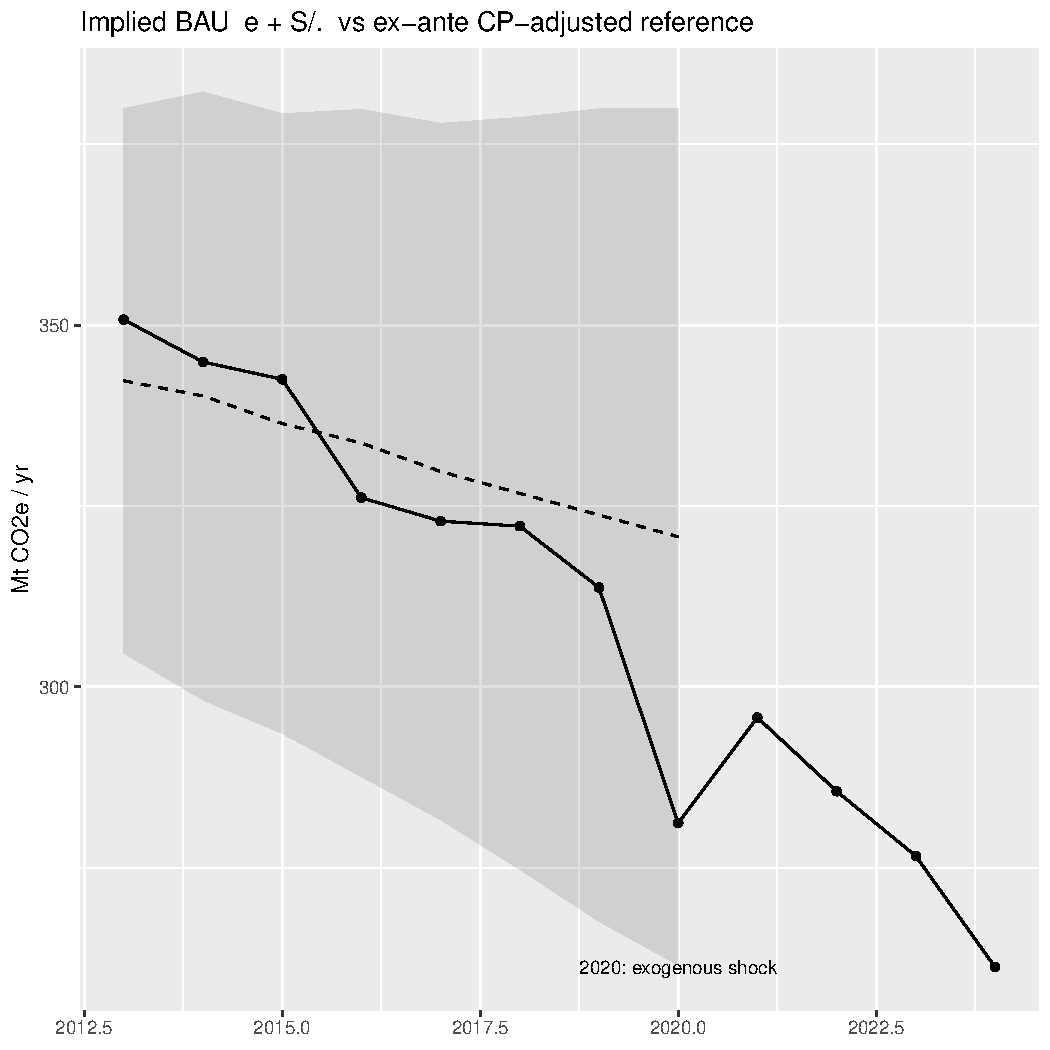
\includegraphics[width=0.5\textwidth]{figures/calib_diagnostic.pdf}
  \caption{Implied BAU emissions $e_t + S_t/\hat\gamma$ (solid) against
  the ex-ante complementary-policy-adjusted reference path (dashed) with
  its $\pm 2\sigma$ forecast fan, 2013--2020; the fan ends at the \citet{borenstein2019}
  horizon and the 2021--2024 points extend beyond it.}
  \label{fig:calibdiag}
\end{figure}
 
\subsection{Numerical solution}\label{sec:solver}
 
The interior equation~\eqref{eq:pde} is solved backward from $T$ on its expected-emissions characteristic slice. The scheme discretizes the $(B,t)$ grid with monotone upwind treatment of the price-dependent $B$-transport $\mu_B=a(t)-y(t)+S/\gamma$, the deterministic net gap $a(t)-y(t)$ carrying the emissions scenario, and imposes the state-constraint clearing condition \eqref{eq:boundary} at $B=0$ inside the time loop; the floor is applied only at output through the envelope, never inside the induction. Emissions uncertainty enters through the simulation layer rather than a diffusion term in the solve: the $y$-sensitivities of Section~\ref{sec:ident} are computed by bump re-solves of the slice, and the projection of Section~\ref{sec:validation} feeds Monte Carlo emissions innovations through the solved surface. Table~\ref{tab:sensitivity} shows this is proportionate: the reported timing is cap-governed and $\sigma_y$-insensitive. The forcing requires one definition made precise. Realized covered emissions embed the abatement response to the realized price path, $e_t=y_t-\Xi(S^{\mathrm{real}}_t)$; a forward emissions scenario extrapolated from realized data therefore embeds a baseline abatement response at an embedded price level $\bar P(t)$, and the feedback must add only the response beyond that baseline: $\Xi^{\mathrm{inc}}=[\min\{S,L\}-\bar P(t)]^{+}/\gamma$, with the clearing value at $B=0$ correspondingly $\min\{\bar P+\gamma(y-a)^{+},\,L\}$. We set $\bar P(t)=R(t)$, exact for a trend anchored on the floor era. Because the central decline rate is fit on 2015--2024, which includes interior years with embedded price above $R$, this choice slightly overstates the incremental feedback. Table~\ref{tab:sensitivity} therefore reports the onset under the alternative $\bar P=1.22\,R$, the window-average embedded level, and the median onset is unchanged at annual resolution: the higher netting baseline reduces cumulative induced abatement by about $17$~Mt, but the self-consistent surface is correspondingly higher and the induced price response offsets most of the reduction.

The un-netted gross feedback $S/\gamma$ is excluded: it double-counts the baseline response embedded in the anchor. The floor enters only at output, through the envelope \eqref{eq:pricerecovery}: projecting onto the floor inside the backward induction would compound the escalator $g_R>r$ into the continuation value and capitalize the carry that Proposition~\ref{prop:cna} bounds, contradicting \eqref{eq:intmartingale}. By the convergence theorem of \citet{barles1991}, the scheme converges to the viscosity solution of the interior problem.

The expected-emissions slice is an approximation whose error we quantify directly. Replacing the diffusion term by the slice misstates the surface by at most $2.8\%$ at the observed states (median $-2.4\%$; symmetric $\pm\sigma_y$ bump bracket), the slice slightly overstating the surface, consistent with the ceiling truncating the up-side clearing values. Carrying the correction through the inversion would move $\widehat{\lambda\ell}$ by roughly $0.002$, the same order as the bank-path robustness noted in Section~\ref{sec:validation}(ii).
 
\subsection{Empirical predictions}\label{sec:predictions}
 
HUH characterize the EU allowance as a strip of binary options on economy-wide emissions, and their three central predictions all follow from that option payoff. Proposition~\ref{prop:dom} removes the payoff. Each row is a positive implication of the substitution mechanism; the benchmark column records the sign under the penalty channel, establishing that the tests discriminate between the two structural candidates rather than holding under any model. A fourth and fifth prediction, with no HUH counterpart, test the vintage structure and the friction decomposition directly.

Table~\ref{tab:predictions} summarizes the five predictions, their sign under the penalty-channel benchmark, and what the data currently say; we then take each in turn.

\begin{table}[H]\centering
\caption{Discriminating predictions: benchmark sign, model sign, and current evidence
status. The penalty-channel benchmark is \citet{hitzemann2018} (HUH); each of the five predictions inverts or has no counterpart under that benchmark, so the same statistic carries opposite signs across the two frameworks. The floor-binding regime (top row) is not a sign inversion but the model's parameter-free structural anchor.}
\label{tab:predictions}
\footnotesize
\begin{tabular}{@{}p{0.235\textwidth} p{0.155\textwidth} p{0.175\textwidth} p{0.305\textwidth}@{}}
\toprule
Prediction & Benchmark (HUH) & This model & Evidence status\\
\midrule
\textit{Anchor:} discrete floor-binding regime; auction marginal, $S=R(t)$ exactly
 & no discrete state & mass point at the reserve (Prop.~\ref{prop:regimes})
 & \textbf{Confirmed, parameter-free.} 9 of 44 joint auctions clear at exactly the reserve, in documented program-risk or demand-collapse episodes (Table~\ref{tab:reserveauctions}, Figure~\ref{fig:premium})\\
\addlinespace[3pt]
Price--volatility relation (Pred.~\ref{pred:volprice})
 & negative ($\rho=-0.46$) & non-negative (no within-regime leverage effect)
 & \textbf{Excludes benchmark value; matches the level.} Interior $\rho=+0.005$ on non-overlapping windows ($n=59$); $95\%$ CI $[-0.32, 0.36]$ excludes HUH's $-0.46$ and contains zero; implied interior volatility $0.255$ vs.\ realized $0.248$, no free parameter\\
\addlinespace[3pt]
Forward-curve slope (Pred.~\ref{pred:curve})
 & backwardation & contango; slope $\approx r$ (interior), $\in[r,g_R]$ (floor)
 & \textbf{Awaiting data.} Multi-maturity CCA settlement curve not public \citep{shi2023}; conjectural\\
\addlinespace[3pt]
Vintage-curve flatness (Pred.~\ref{pred:vintage})
 & current-vintage premium & flat, $S^{\mathrm{adv}}/S^{\mathrm{cur}}\approx1$
 & \textbf{Supported, sign only.} Constant regression $-0.08\%$/yr (HAC s.e.\ $0.28$) over $27$ interior auctions; CI excludes the penalty-channel premium for any shortfall probability above $1.5\%$; regime-dependent dispersion as predicted\\
\addlinespace[3pt]
Speculative positioning by regime (Pred.~\ref{pred:positions})
 & no counterpart & co-moves with regime; small/short at floor, long in interior
 & \textbf{Supported; trend-following rejected.} Spearman $\rho=+0.53$ ($n=44$), permutation $p=0.0003$; trailing-return loading $-1.26$ ($t=-2.53$) rejects trend exposure by sign; regime vs.\ level separated by the touch responses\\
\addlinespace[3pt]
Option-implied volatility smile (Pred.~\ref{pred:smile})
 & downward (equity-like) & upward (commodity-like)
 & \textbf{Awaiting data.} No liquid public CCA option panel; directional check for future work\\
\bottomrule
\end{tabular}

\smallskip
{\footnotesize\justifying
\textit{Notes.} ``Excludes benchmark value'' denotes a confidence interval excluding the penalty-channel point value ($\rho=-0.46$), though not every negative value; ``supported'' denotes a correctly-signed test whose formal power is otherwise limited; ``confirmed, parameter-free'' is reserved for the auction anchor, which is a primary-market fact requiring no calibrated parameter; ``awaiting data'' denotes a prediction that is not yet testable on public data. The positioning test is the most independent of the five, as positioning is an observed series rather than a price transform.\par}
\end{table}

\emph{The empirical anchor: a discrete floor-binding regime.} The model's most directly observable structural claim is the existence of the floor-binding regime of Proposition~\ref{prop:regimes} as a discrete state, and two facts carry it, which we state in turn. The first is distributional and parameter-free: across the 44 joint auctions with comparable reporting (2015Q2--2026Q1), the premium-over-reserve distribution has a mass point at exactly zero. Nine auctions settled at the Auction Reserve Price to the cent on the current-vintage leg, the mechanical signature of an undersubscribed auction rationed at the reserve; in seven of the nine the advance leg also settled at the reserve exactly, and in the remaining two (August 2020, May 2025) it settled $0.3\%$ and $1.1\%$ above it while the current leg was rationed. The other thirty-five auctions cleared strictly above the reserve. The mass point itself is a property of the auction institution: rationing at the reserve arises mechanically under Lemma~\ref{lem:floor} whatever determines bid values, so it does not by itself discriminate the pricing channel. Its evidential content is twofold: it certifies, with no calibrated parameter, that the floor-binding regime of Proposition~\ref{prop:regimes} is a realized discrete state rather than the tail of a continuum; and it supplies the regime classification used throughout this section without reference to the fitted model, so no regime-conditional result below rests on a model-based partition of its own sample. The second fact is the timing. The nine clearings fall in the 2016Q1--2017Q1 \emph{CalChamber} litigation window (five consecutive auctions), the 2020 pandemic demand collapse (two auctions), and two isolated 2025--26 touches under federal regulatory threat (Table~\ref{tab:reserveauctions}): seven in documented episodes of program-survival risk and two under a demand collapse. The model does not treat these two shocks alike, and Prediction~\ref{pred:positions} is where the data discriminate them: positioning unwinds at the demand touch and persists at the survival touches.

Two clarifications complete the anchor. First, the regime observable. In the primary market the floor regime is identified by the $0$--$1.7\%$ premium cluster (sixteen auctions), within which settlement at exactly the reserve marks the episodes in which rationing was strict; the daily state-path classification of Section~\ref{sec:validation}(i), which places 2013--2020 in the floor regime throughout, refers to this cluster, not to the exact-zero subset alone. Second, the distribution additionally contains an empty band: no auction settles between $1.7\%$ and $3.5\%$ (Figure~\ref{fig:premium}), so the floor cluster and the interior continuum are separated by a region the data leave vacant. An empty interval of this relative width occurs somewhere in the support with probability $0.78$ under a lognormal density fitted to the 35 strictly positive settlement premia. We therefore read the gap as descriptive rather than evidential and rest the anchor entirely on the mass point, which requires no such qualification. This, rather than any price-level fit, is the empirical core of the section.
 
\begin{prediction}[Price--volatility relation]\label{pred:volprice}
The WCI spot price and its instantaneous volatility are non-negatively related, reversing the leverage effect HUH document for the EU ETS. 
\end{prediction}
 
\noindent\emph{Mechanism.} HUH's negative relation arises because the low-price state is the near-the-money region of the binary option, where convexity makes volatility high. Under the substitution channel the low-price state is instead the floor-binding regime, where $S(t)=R(t)$ follows a deterministic escalator and instantaneous volatility is suppressed toward zero; positive volatility appears only in the interior-Hotelling and boundary-clearing regimes, where prices are higher. Low price thus coincides with low volatility. 

\emph{Test (excludes the benchmark value).} The relevant null is not zero but the benchmark: HUH estimate $\rho=-0.464$ for the EU ETS, and the prediction is that the WCI interior carries no such leverage effect. On the 2021--2026 interior sample, the rank correlation between the spot price and 21-day realized volatility computed on non-overlapping windows ($n=59$ independent observations) is $\rho=+0.005$, with a stationary-bootstrap $95\%$ interval of $[-0.32,\,0.36]$. The interval excludes the benchmark value while containing zero and, at its lower edge, moderate negative values: the test rejects the estimated EU-ETS leverage effect rather than any negative relation, which is exactly the prediction. Interior volatility is news-driven and level-independent, consistent with \eqref{eq:intmartingale}, and carries none of the negative dependence the penalty channel would generate.\footnote{For completeness: the floor-era value is $\rho=+0.24$ (2013--2017), computed on a spliced price proxy (Appendix~\ref{app:splice}) at a floor where model volatility is near zero, and the pooled value is $\rho=0.70$ ($n=2{,}506$, 2013--17 and 2021--26 daily), which is partly mechanical: pooling a low-price, low-volatility floor cluster with a high-price, high-volatility interior cluster manufactures positive correlation. We report both as the cross-regime contrast that is the prediction's mechanism; neither is the test.}

The surface supplies a quantitative companion to the sign test. Combining the solved emissions sensitivity with the independently calibrated $\sigma_y$ gives a model-implied interior volatility of $\sigma_y\,\partial_yS/S=0.255$ (median over the interior dates; IQR $[0.233,0.277]$), against a realized annualized volatility of $0.248$ on the same sample. This is a moment the model was not fit to, generated with no free parameter. The implied figure is the emissions-news component at fixed $\lambda\ell$; that it approximately exhausts realized volatility is consistent with the reading of Section~\ref{sec:validation}(ii), in which the daily wedge path itself partly carries emissions news relative to the projected state. The same sensitivity, read as premium capacity, is what the bound of Section~\ref{sec:ident} prices: the quantity of emissions risk on the surface is thereby measured, and only its market price $\lambda_y$ remains free.
 
\begin{prediction}[Forward curve slope]\label{pred:curve}
The WCI inter-temporal forward curve is in contango in the interior regime, with a regime-diagnostic slope. In the interior-Hotelling regime the slope is $\approx r$. In the floor-binding regime it lies in $[r,g_R]$, equal to $r$ plus the capitalized capacity multiplier, and the gap to $g_R$ measures program-risk compensation.% multi-contract settlement panel required? front-month splice contains no cross-section
\end{prediction}
 
\noindent\emph{Mechanism.} HUH predict backwardation as the normal state because the spot carries a current-period scarcity value the forward does not. With that value absent, the curve is set by $F_t(T)=\E_t^{\Qmeasure}[S_T]$, which spot-market frictions do not distort. In the interior regime, Proposition~\ref{prop:cna}(iii) gives a slope of $r$. In the floor-binding regime the futures price is the survival-weighted expectation, so the slope equals $r$ plus the capitalized capacity multiplier $\int_t^Te^{-r(s-t)}\E_t^\Qmeasure[\eta_s]\,ds$. With $\eta\approx0$ the curve slopes at $\approx r$ even while the conditional escalator drifts at $g_R$, and the gap between the escalator and the curve slope prices $\lambda\ell$. The same structure extends to the interior: conditional on survival the pre-jump value drifts at $r+\lambda\ell$ (Proposition~\ref{prop:intpricing}), while $F_t(T)=\E_t^{\Qmeasure}[S_T]$ embeds the jump. The curve slope therefore remains $\approx r$ in both regimes, and the realized-minus-implied drift gap on the interior measures $\lambda\ell$ directly, an out-of-sample check on the level-fitted value of Section~\ref{sec:ident}.

The implied cash-and-carry basis $F-Se^{r\tau}>0$ is not an arbitrage, because the long-spot leg is capped by the holding limits of Assumption~\ref{ass:capacity} and the reverse trade requires an infeasible spot short (Corollary~\ref{cor:carry}). Because $r$ and $g_R$ are both observable, the two predicted slopes are not free parameters: the curve over-identifies the model. The decomposition \eqref{eq:eta-r1} has a peso-problem signature: conditional on survival, realized floor-regime holding returns approximate $g_R$, while the futures-implied expected return approximates $r$. A caveat sharpens what the test identifies. \citet{quemin2021} show that EU~ETS banking dynamics are reconciled with futures-implied discount rates only under rolling finite planning horizons, with implied rates above $r$. Prediction~\ref{pred:curve} is therefore a joint test of the substitution channel and full intertemporal optimization. An interior-regime slope persistently above $r$ with a positive bank and slack capacity would indicate bounded-horizon discounting in the sense of Quemin--Trotignon rather than a revival of the penalty channel, and we read the curve evidence with that alternative on the table.

\emph{Evidence (data-limited; conjectural).} A direct test requires the multi-maturity secondary-market futures settlement curve, which is not publicly available for CCA contracts: \citet{shi2023} document that vintage-level CCA
futures data are not public, and the available series is a single rolled front-contract index with no cross-sectional slope. We therefore treat Prediction~\ref{pred:curve} as conjectural pending secondary-curve data. We do not read the advance-auction spread (Prediction~\ref{pred:vintage}) as a proxy for this slope: both auction legs settle at the auction date and so carry no money-carry, and the advance leg is a thin primary-issuance instrument rather than a traded forward. The \citet{quemin2021} bounded-horizon alternative is the relevant competing hypothesis once curve data exist, and we flag it as such.

\begin{prediction}[Vintage curve flatness]\label{pred:vintage}
The same-date price schedule across allowance vintages is flat in the interior regime: the advance-auction settlement equals the current-auction settlement up to a negligible usability discount, $S^{\mathrm{adv}}/S^{\mathrm{cur}}\approx 1$, against the systematic current-vintage premium implied by the penalty channel.
\end{prediction}

\noindent\emph{Mechanism.} Both auction legs are paid at the auction date, so no money-carry slope appears in the vintage dimension; this isolates the value of the allowance itself from the time value of money, which appears only in the futures curve of Prediction~\ref{pred:curve}. Under unlimited banking the current vintage weakly dominates the advance vintage: it is usable immediately and later, the advance only from its vintage year. The spread therefore prices the usability option over the three-year window, whose value is the expected convenience yield $\int_t^{t+3}e^{-r(s-t)}\E_t^{\Qmeasure}[\nu_s]\,ds$. With $\Prob_t\{\text{shortfall}\}=0$ and a chronically positive bank, $\nu\equiv 0$ within the window and the schedule is flat. The bound is one-sided. $S^{\mathrm{cur}}\geq S^{\mathrm{adv}}$ would be enforced by arbitrage only through a short of the advance leg, which is infeasible (Assumption~\ref{ass:capacity}; a fortiori at primary auction). The flat schedule is therefore the equilibrium only where neither leg is supply-rationed: when a current-auction supply limit binds, marginal demand spills onto the advance leg, $S^{\mathrm{adv}}$ is bid above $S^{\mathrm{cur}}$, and no admissible trade corrects it. An advance premium is thus a predicted signature of a binding current-auction purchase limit, not a violation of the bound. Under the penalty channel, the current vintage carries the near-dated strip of compliance-shortfall options that the deferred vintage lacks, implying a current-vintage premium that widens with scarcity risk.

\emph{Test (supporting, sign only; regime-dependent dispersion).} Regressing $\log(S^{\mathrm{adv}}/S^{\mathrm{cur}})$ on a constant over the $27$ interior auctions\footnote{Interior auctions are those settling above the vacant band of Figure~\ref{fig:premium}; the single auction whose advance leg settled at the reserve, February 2022, is excluded as censored, leaving 27 of the 28 above-band auctions.} gives $-0.08\%$ per year of deferral (HAC standard error $0.28$; $95\%$ CI $[-0.64,\,0.48]$), statistically and economically flat, consistent with $\nu\equiv0$ over the usability window. The flatness is not an artifact of pooling across the 2021 backstop change: the pre-ceiling and post-ceiling interior subsamples give $-0.31\%$ and $+0.05\%$ per year respectively ($n=10$ and $17$), both indistinguishable from zero. For the alternative to have content it needs a magnitude. Under the penalty channel the current-vintage premium is bounded below by the discounted value of the near-dated shortfall-option strip, $e^{-r\bar\tau}\,p_{\mathrm{short}}\,(\bar p/S-1)/3$ per year of the window, about $1.6\%$ per year at a shortfall probability of only $5\%$ and a penalty-to-price ratio of two. The confidence interval excludes this bound for any shortfall probability above $1.5\%$. Across the full 2015--2026 sample the advance leg is backwardated relative to the current in 19 of 31 non-censored auctions, a majority carrying the penalty channel's predicted sign; the one-sided arbitrage bound explains why this cannot be corrected (a short of the advance leg is infeasible), and the regression shows the magnitude is economically negligible. The flat central tendency conceals large regime-dependent dispersion, which is itself the diagnostic. The December 2021 advance premium ($+20\%$ in level) is the supply-rationing signature just described, the per-auction purchase limit having bound in the current auction. The February 2022 advance collapse toward the reserve ($-32\%$) carries vintage-specific program risk, the survival channel of Remark~\ref{rem:2016} operating across vintages. We read the central flatness as supporting the no-convenience-yield prediction and the dispersion as loading on the frictions of Assumptions~\ref{ass:capacity} and~\ref{ass:jump}, not as evidence on the money-carry curve.

\begin{prediction}[Speculative positioning by regime]\label{pred:positions}
Net speculative futures positioning co-moves with the pricing regime: small or net short in the floor-binding regime, large and long in the interior regime, with positioning anticipating regime transitions. At transient floor touches, positioning distinguishes the shock: it unwinds when the shock is to demand (2020) and persists when the shock is to program survival with interior scarcity value intact (April 2025, February 2026). Aggregate speculative holdings sit strictly inside the regulatory capacity bound in the floor regime, identifying the floor-regime excess return of Corollary~\ref{cor:carry} as program-risk compensation ($\eta\approx 0$) rather than a binding-limit shadow price; the capacity channel binds episodically through auction purchase limits in demand spikes at regime transitions.
\end{prediction}

\noindent\emph{Mechanism.} If the floor carry were a capacity-constrained arbitrage, speculative length would be pinned at $\bar H(t)$ precisely when the carry is widest, i.e.\ throughout the floor regime. If it is risk compensation, length is small when program risk is elevated and grows with interior-regime scarcity value. The two channels of \eqref{eq:eta-r1} thus have opposite positioning signatures in the same data.

\emph{Test (independent; positioning is not a price transform).} The data are the CFTC disaggregated Commitments of Traders, all CCA vintage contracts 2013--2026; net positioning is managed money plus other reportables. The test proceeds in three steps: the regime co-movement, the exclusion of a trend-following alternative, and the touch-by-touch discrimination that separates the regime mechanism from a generic level exposure.

\emph{Step 1: co-movement.} Net positioning co-moves with the regime's primary-market observable, the settlement premium over the reserve: Spearman $\rho=0.53$ ($n=44$), and $\rho=0.70$ ($n=42$) excluding the 2025--26 transient policy-shock floor touches that the prediction classifies as a distinct case.\footnote{Operationally, the touches are the auctions with premia below $2\%$ and net length above $60$~Mt---floor-proximate settlements at which positioning persisted, the program-risk signature the prediction classifies separately. The 2020 demand-collapse touches fail the second condition (positioning unwound) and remain in the sample.} The permutation $p$-values are $0.0003$ and $2\times10^{-5}$ respectively ($N_{\mathrm{perm}}=50{,}000$ reshuffles of positioning across auctions; null distribution centered at zero with a $95\%$ range of $[-0.30,+0.30]$). We use a permutation test rather than a bootstrap because auction dates are non-overlapping: positioning and regime are exchangeable under the null of no association, so reshuffling is a valid draw from that null, unlike the overlapping-window correlation of Prediction~\ref{pred:volprice}, where the sign remains the test. Because positioning is an independent series rather than a price transform, the co-movement is not subject to the near-circularity of the implied-$\lambda\ell_t$ fit. It also identifies the sign of the floor-regime decomposition: speculative length sits strictly inside any plausible aggregate capacity bound throughout the chronic floor era (2013--2020), placing $\eta\approx0$ and attributing the floor-regime excess to program risk. The capacity channel binds only episodically, through the per-auction purchase limit; in December 2021 gross length peaked at its sample-to-date maximum at the auction date and unwound sharply thereafter. We read this as identifying the decomposition's sign, not as a structural estimate of $\lambda\ell$.

\emph{Step 2: the trend-following alternative.} Managed-money positioning co-moves with price level and trend under trend-following exposure alone, in any model, so this generic alternative must be excluded before the co-movement identifies the mechanism. Trend-following has a signed implication: positioning loads positively on trailing returns. The data reject it directly. Regressing net positioning on the regime indicator, the trailing twelve-month return, and the log price level (HAC standard errors, $n=44$; trailing return computed on the continuous spliced daily series of Appendix~\ref{app:splice}) gives a trailing-return coefficient of $-1.26$ ($t=-2.53$): positioning falls after price run-ups, the opposite of trend exposure, and within the interior it is contrarian in the direction the Hotelling martingale implies, since a dip below the interior value raises the expected holding return.

\emph{Step 3: the touches.} The same regression cannot separate the regime from the price level (regime coefficient $0.15$, $t=0.82$; the sign itself is not stable across price-series choices, underscoring the point): the interior era is the high-price era by construction, so the two regressors are nearly the same partition of forty-four dates, and no coefficient allocation should be read into either. The discrimination is carried instead by the floor touches, where the hypotheses disagree. Any level- or trend-based rule predicts uniform behavior across touches, all of which follow price declines to the same floor; the model predicts unwinding at the 2020 demand touch and persistence at the 2025--26 survival touches. The data show the model's pattern.

\begin{prediction}[Volatility smile]\label{pred:smile}
The CCA option-implied volatility smile is upward-sloping (commodity-like), in contrast to the symmetric/downward (equity-like) smile HUH predict for the EU.
\end{prediction}
 
\noindent\emph{Mechanism.} HUH's downward smile is induced by the binary-option convexity under the physical measure. Treating the allowance as a storable commodity with the regulatory floor as a reflecting lower barrier truncates the left tail of the risk-neutral price density: downside is capped at $R(t)$ in the baseline regime where the auction is marginal (Lemma~\ref{lem:floor}), so puts struck near the floor carry little value and the smile slopes upward. This is the commodity-market shape that HUH explicitly note stands against their equity-like result.

\emph{Test (candidate, data-permitting).} The same floor-as-barrier truncation that sets the forward-curve slope of Prediction~\ref{pred:curve} fixes the sign of the smile here, on a different instrument: the curve identifies it in the drift of $F_t(T)$, the smile in the left tail of the risk-neutral density. The predicted smile slope is positive. No liquid public CCA option panel currently exists, so this is a directional check for future work rather than a result; we state it because the mechanism pins the sign in advance, and a panel, once available, confirms or falsifies it cleanly.

\noindent We summarize the contrast in Figure~\ref{fig:surface}: under WCI rules the price, as a function of the bank, falls smoothly from the scarcity-clearing edge to the discounted floor and never develops the binary step that signals the penalty channel of \citet{hitzemann2018}; the only non-smoothness is the convex kink where it meets the escalating floor.

\begin{figure}[H]
  \centering
  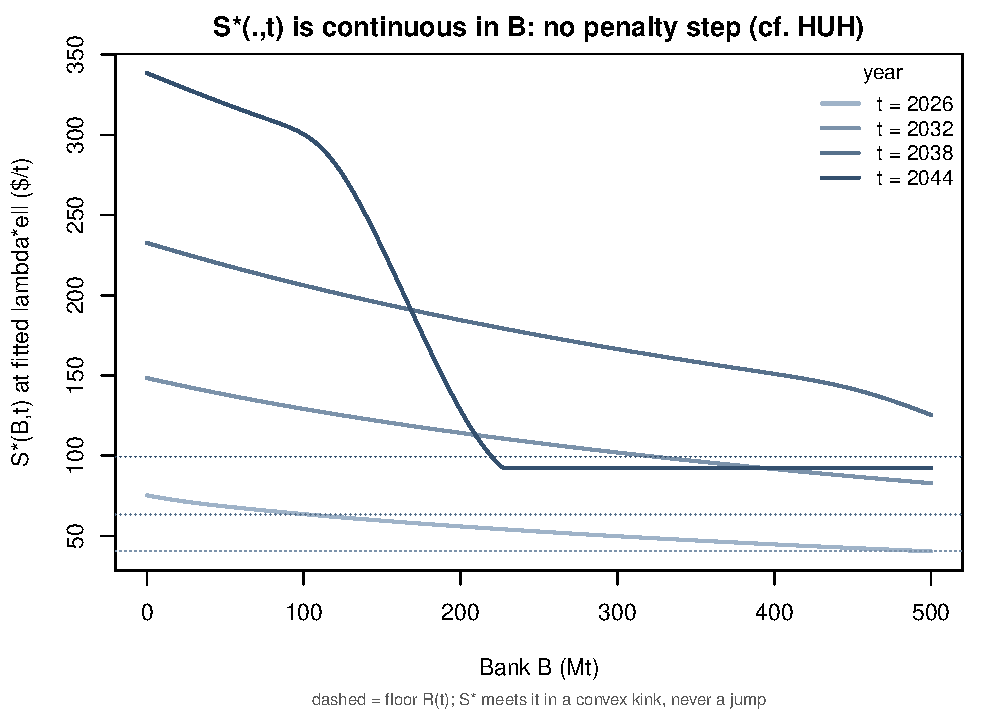
\includegraphics[width=0.72\textwidth]{figures/figure_surface_slices.pdf}
  \caption{Equilibrium price surface $S^{\star}(\cdot,t)=\max\{S^{\mathrm{int}},R\}$ as a function of the bank $B$ at four horizons, under expected emissions, the adopted cap, and the fitted discount wedge $\lambda\ell=0.10$. The price is continuous in $B$, meeting the escalating floor $R(t)$ (dashed) in a convex kink rather than the discrete step that the penalty channel of \citet{hitzemann2018} would produce. The absence of a step is the substitution channel's structural signature.}
  \label{fig:surface}
\end{figure}
 
\subsection{Validation design}\label{sec:validation}
 
We assess the calibrated model in three steps; later steps carry more evidential weight than earlier ones.
 
\emph{(i) Regime classification.} The discrete floor-binding regime is confirmed directly in the auction record (the empirical anchor above), with no calibrated parameter. Applying the same classification along the realized daily state path recovers the historical sequence: a premium over the reserve in the earliest years of a then-illiquid market, convergence to the floor with the 2016--2017 below-floor episode (Remark~\ref{rem:2016}), floor-proximate settlements through 2020, lift-off to the interior in 2021, and the transient floor touches of 2020 and 2025--26. The flow identity dates these transitions against the bank: the private bank grew essentially monotonically through the sample, from 321.1~Mt at the 2020/21 boundary to 379.1~Mt at end-2024 and $\approx403$~Mt at the launch state, so the sub-floor episode and the lift-off occurred at large and rising $B$ and load on the forward arguments of the scarcity value (expected-cap revisions and movements in $\lambda\ell$). The model accommodates cap revisions as discrete re-solves under the updated $a(t)$; a stochastic-regulator extension endogenizing cap news is left to future work.
 
\emph{(ii) Program-risk event response.} The interior specification of Proposition~\ref{prop:intpricing} turns the level into a daily implied series. Inverting the observed secondary price on the risk-adjusted surface, $P_t=S^{\mathrm{int}}(B_t,t;\lambda\ell_t)$, gives a daily implied interior discount wedge $\lambda\ell_t$ on the 1{,}253 interior dates of 2021--2026 (Figure~\ref{fig:lambda}).\footnote{The inversion conditions on the projected bank path; re-running it on the CIR-interpolated observed bank moves the median from $0.100$ to $0.099$ and neither event delta by more than $0.001$, so the choice is immaterial.} The path, not the point, carries the information: $\lambda\ell_t$ runs near $0.08$--$0.10$ through 2021--2023, troughs at $0.076$ at the early-2024 price peak, and climbs by roughly sixty percent from mid-2024 to $0.154$ at the end of the sample. The ascent begins with the 2024 rulemaking delays, ahead of the federal threat. Because the forcing is deterministic, the implied path bundles emissions news relative to the projected state with program risk; the event windows, not the path level, carry the risk identification. As scoped at the top of the section, the daily $\lambda\ell_t$ is, conditional on the state path, a re-expression of the price; the content of the inversion is the level (one parameter reconciling the price with a surface whose scale is fixed by statute, cap arithmetic, and engineering abatement costs rather than by prices) and the units, which make the discount commensurable with the floor-carry value of Corollary~\ref{cor:carry} and with reduced-form credit magnitudes. We probed the path for external content against newspaper-based climate-policy-uncertainty indices \citep{gavriilidis2021}. Monthly innovations are uncorrelated across index variants: $|\rho|\le0.10$ over the 53--56 innovations through late 2025, against a five-percent critical value near $0.26$. This is consistent with the bundling caveat above, at monthly frequency the path being dominated by demand news relative to the deterministic forcing rather than by measured policy uncertainty, though a null on 56 noisy innovations has little power against moderate true association. The reading of the level as program risk therefore rests on the event-window signs, the cross-claim ordering below, and the designated post-adoption test, not on the path itself. The 2025 events move it with the correct signs: the $\pm30$-day delta is $+0.0125$ around the April 2025 federal executive action and $-0.0068$ around the September 2025 AB~1207 reauthorization. To attach inference, we compute the same $\pm30$-day delta at every admissible interior date; against this placebo distribution ($n=1{,}186$ windows) the April delta falls at the $99.6$th percentile and the September delta at the $4.7$th; the placebo windows overlap, so these are benchmark ranks rather than exact $p$-values, but both events sit in the correct tail.

The event responses are consistent with the positioning evidence of Prediction~\ref{pred:positions}, where the same touches register as program-risk rather than demand shocks. Two caveats scope the reading. First, the surface conditions on the cap adopted on 28~May 2026, while the market before that date priced an adoption still uncertain. Every fitted value here is pre-adoption, so the upper-bound reading applies to the whole path, which bundles cap-adoption probability with durability risk. The adoption is therefore a designated out-of-sample test with the sign pinned in advance. If the pre-adoption level mostly priced adoption uncertainty, the implied discount collapses toward the floor-carry value of $0.03$ once the cap is law; if it priced program durability, it persists near $0.10$--$0.15$ with the cap known. Persistence alone is also consistent with the emissions-premium component bounded in Section~\ref{sec:ident}, so the sharper out-of-sample object is the delta in the adoption window itself, an event on which a premium over a slow state variable does not move. The claim-specific-loss decomposition sharpens this into a three-way prediction: post-adoption, the floor-carry reading of Corollary~\ref{cor:carry} should remain near $0.03$ while the interior reading persists near $0.10$--$0.15$, so the cross-section of the two claims, and not only the level, is testable once the August 2026 auction prints. The May 2026 auction, held days before the vote, inverts at $0.16$, the sample maximum, with the primary market compressed to within $3.1\%$ of the reserve, inside the vacant band of Figure~\ref{fig:premium}, which no in-sample auction enters. The August 2026 auction supplies the first post-adoption print; either outcome is informative for the decomposition of Corollary~\ref{cor:carry}. Second, the same survival process read on two claims gives discounts differing by a factor of three: the floor-carry decomposition of Corollary~\ref{cor:carry} puts $\lambda\ell\approx g_R-r\approx0.03$ on the 2013--2020 floor claim, against $0.10$ on the 2021--2026 scarcity claim. The ordering is what claim-specific loss implies. A curtailment that softens the cap without killing the program destroys the scarcity claim ($\ell$ near one on $S-R$) while leaving the floor claim nearly whole ($\ell$ near zero on $R$), so a single intensity $\lambda$ delivers exactly this ranking of $\lambda\ell$ across claims. The wedge bound of Section~\ref{sec:ident} offers a complementary reading of the same ordering: a priced emissions premium loads only on the scarcity claim, since the floor claim carries no $y$-exposure, and so widens the same gap. The two readings are observationally equivalent on the level and are separated, again, only by the event responses. Bounded planning horizons in the sense of \citet{quemin2021} are the observationally equivalent alternative for the level, as flagged at Prediction~\ref{pred:curve}, though they do not by themselves produce the event co-movement.

\begin{figure}[H]
  \centering
  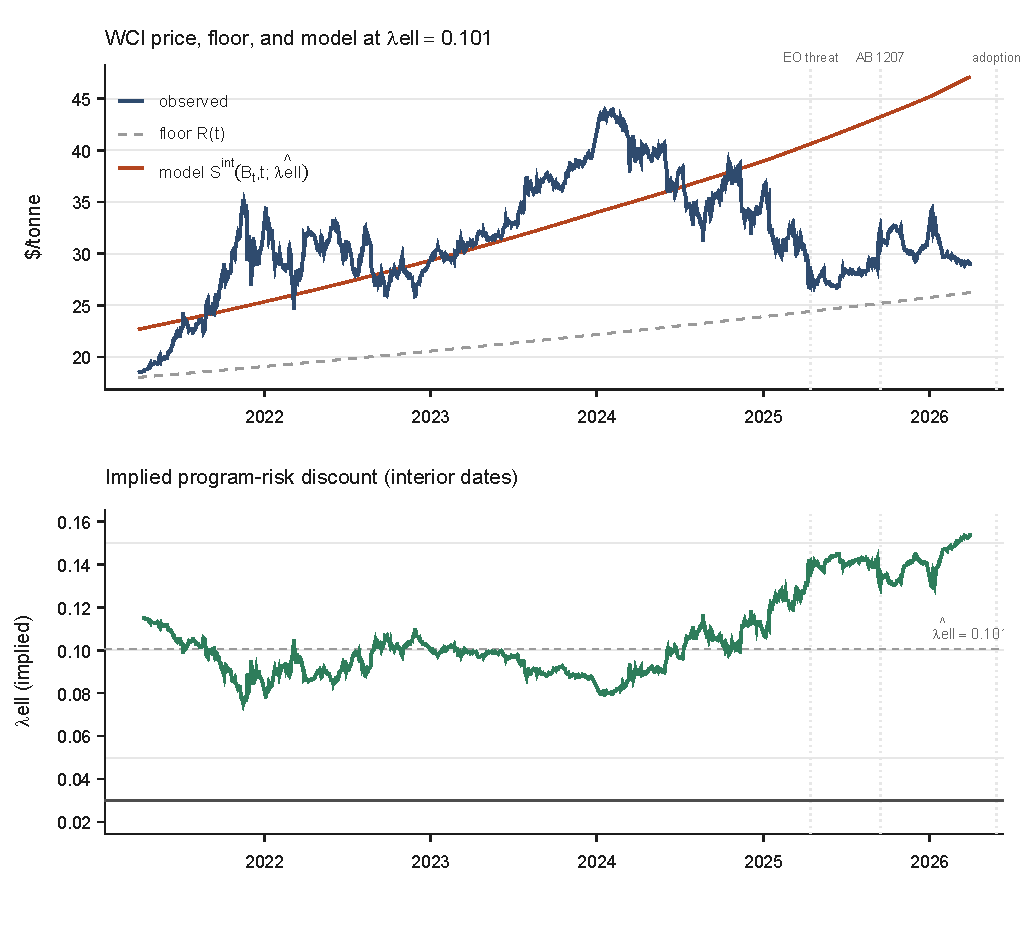
\includegraphics[width=0.80\textwidth]{figures/figure_lambda.pdf}
  \caption{Top: observed WCI secondary price, the floor $R(t)$, and the risk-adjusted interior value $S^{\mathrm{int}}(B_t,t;\widehat{\lambda\ell})$ at $\widehat{\lambda\ell}=0.10$. Bottom: the daily implied discount wedge $\lambda\ell_t$, the price restated as a per-year discount on the risk-adjusted surface; reference line at the floor-carry value $0.03$ (Corollary~\ref{cor:carry}). Dotted verticals: April 2025 federal executive action and September 2025 AB~1207 reauthorization; the sample ends 31~March 2026, before the Cap-and-Invest adoption.}
  \label{fig:lambda}
\end{figure}
 
\textit{(iii) Forward projection.} We project the private bank forward from its CIR-validated end-2024 level, $B(2024) = 379.1$~Mt, under the flow identity
\begin{equation}
  dB(t) = a(t) - \bigl[\,e(t) - o(t)\,\bigr],
  \label{eq:bankflow}
\end{equation}
where $a(t)$ is the CARB Table 6-2 allowance budget, $e(t)$ covered emissions, and $o(t)$ offset surrender (bank-neutral from December~2027). The launch state $B(2026)\approx403$~Mt follows from the validated 2024 anchor through the 2025--26 flows, which we make explicit: allocation $a(2025)=267.4$~Mt under the pre-amendment budget, covered emissions $e(2025)=249.3$~Mt (the central-scenario value; MRR 2025 is unpublished at the sample freeze), offset surrender $o(2025)=6.0$~Mt, and zero net partial-year 2026 flows, the launch state being the start of 2026 (Table~\ref{tab:bridge}).
We anchor on the validated level rather than on a fitted bank value, and we report the projection in three feedback variants that bracket the price-abatement response.

\begin{table}[H]\centering
\caption{Bridge from the CIR-validated end-2024 bank to the projection launch state.}
\label{tab:bridge}
\footnotesize
\begin{tabular}{@{}l r@{}}
\toprule
 & Mt\\
\midrule
$B(2024)$, CIR-validated & $379.1$\\
$+$ allocation 2025 & $267.4$\\
$-$ covered emissions 2025 & $249.3$\\
$+$ offset surrender 2025 & $6.0$\\
$\pm$ partial-year 2026 flows (launch at start of 2026) & $0.00$\\
\midrule
$B(2026)$, launch & $\approx 403$\\
\bottomrule
\end{tabular}

\smallskip
{\footnotesize\justifying
\textit{Notes.} $a(2025)$ is the pre-amendment vintage budget; $e(2025)$ is the central-scenario value, MRR~2025 being unpublished at the freeze; $o(2025)$ from CIR differencing (Section~\ref{sec:data}).\par}
\end{table}
The exogenous variant sets induced abatement to zero and is model-independent. The risk-adjusted variant feeds back the incremental abatement $[\min\{S,L\}-R]^{+}/\gamma$ from the self-consistent surface at the fitted $\lambda\ell=0.10$. Because the feedback sits inside the bank drift of the solve, the surface is self-consistent in the state by construction and the projected path is its characteristic; no outer fixed-point iteration arises. The frictionless variant ($\lambda\ell=0$) feeds back from the certain-program surface, on which the price sits at the discounted exhaustion-date ceiling, $S(t)=e^{-r(\tau^{*}-t)}L(\tau^{*})$. On that surface the feedback runs at its ceiling cap $(L-R)/\gamma$ throughout, the maximal response the ceiling admits. The exogenous variant is the early edge, the frictionless variant the late edge, and the risk-adjusted variant the model's own point.

Because realized emissions and the abatement decomposition are not separately identified, we project covered emissions directly rather than through a BAU/abatement split. We anchor on realized 2024 covered emissions ($256.6$~Mt) and apply a proportional decline rate, reporting the onset distribution across a scenario band. The central rate, $-2.87\%$/yr, is the log-linear trend fit to post-expansion covered emissions (2015--2024, excluding the 2020 pandemic year): it is the realized pace of the capped sectors, estimated, not assumed. The band brackets this with a slower $-2.0\%$/yr and a faster $-4.5\%$/yr, the latter the proportional image of the realized 2021--2024 pace ($-11.7$~Mt/yr at the 2024 level). This band also spans the policy-relevant range. California's statutory trajectory, $40\%$ below 1990 by 2030 and $85\%$ below by 2045 \citep{sb32, ab1279}, implies, for the covered sectors, a
decline at least as steep as the realized pace and plausibly steeper, placing the legislated path in the faster half of our band. Because slower decline exhausts the bank earlier (the comparative static below), the realized-pace central is the early-exhaustion case and the steeper policy-implied path the later one. The 2034--2038 onset window is therefore robust to whether the capped sectors merely sustain their historical pace or accelerate toward the statutory target. The proportional specification is preferred on the grounds of Section~\ref{sec:ident}; the functional-form choice, not the within-fit standard error, is the binding source of timing uncertainty.

The result (Figure~\ref{fig:projection}) is robust in direction and bounded in timing, though its precision should not be overstated. The binding uncertainty is the emissions-decline scenario and the functional form, not the within-scenario sampling noise; we therefore report the result as a range across scenarios rather than as a point estimate with a Monte-Carlo band. The bank exhausts within the horizon across the entire scenario range short of an unprecedented decline: median onset under the central decline ($-2.87\%$/yr) is 2034 exogenous, 2036 risk-adjusted, and 2036 frictionless; under slow decline ($-2.0\%$/yr) the variants give 2033, 2034, and 2035; under fast decline ($-4.5\%$/yr, the proportional image of the steepest realized pace) they give 2038, 2041, and 2045. The feedback defers onset by one to three years at the fitted discount wedge, and the central window is 2034--2036 across the bracket. Exhaustion is avoided only under sustained proportional decline steeper than roughly $6\%$/yr in the exogenous and risk-adjusted variants: at $-6\%$ the bank survives to 2045 in about half the exogenous simulations, and at $-8\%$ with near-certainty. Only the frictionless edge, on which induced abatement runs at the ceiling cap from the outset, lowers the threshold toward the realized-record pace, and even there the bank exhausts by 2045 in about half of the paths at $-4.5\%$/yr. Within-horizon exhaustion is thus the robust prediction and escape the tail case. The onset distribution is narrow because the post-2027 cap--emissions deficit is so large ($a-y\approx-60$ to $-110$~Mt/yr) that a $\sigma_y=20$ annual shock moves onset by at most a year: exhaustion timing is governed by the cap, not by emissions volatility. The direction is the model's comparative static: slower decarbonization drains the bank earlier, because the cap tightens regardless and a slow-abating economy meets a shrinking allocation with a larger deficit. The escape threshold is the same static read forward: escape requires absolute abatement that keeps pace with the collapsing cap, which under proportional decline demands an accelerating percentage rate that convex adjustment costs make implausible. The up-to-118~Mt of above-cap MDI allowances, if fully taken up, shift onset out by one to two years (central to 2035, fast to 2040) and form the late edge of the band. The iid-noise specification is conservative, since persistent emissions would widen the distribution. This reverses a flat-cap reading under which within-horizon scarcity was near zero: under the legislated declining cap the boundary regime is a central, near-term prediction. We summarize the projection accordingly: across every decline scenario short of a sustained $\geq6\%$/yr pace, which is steeper than anything yet realized in the program, and across the full feedback bracket, the bank exhausts before the 2045 horizon, with a central window of 2034--2036. The $[5\%,95\%]$ bands of Table~\ref{tab:sensitivity} measure only the $\sigma_y$ contribution within a fixed scenario and understate total uncertainty by construction; the scenario range, not those bands, is the relevant measure of uncertainty.


\begin{figure}[H]
  \centering
  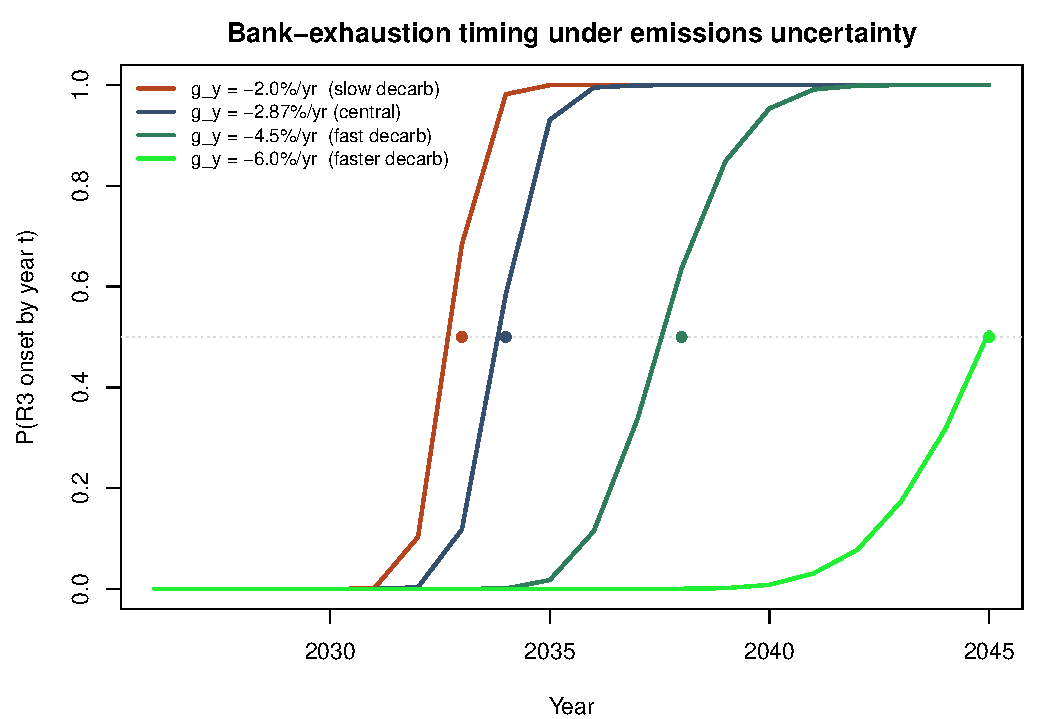
\includegraphics[width=0.80\textwidth]{figures/figure_projection.pdf}
  \caption{Regime~3 (boundary-clearing) onset under emissions uncertainty. Each curve is the simulated probability that the bank reaches zero by year $t$, starting from $B(2026)\approx403$~Mt under the adopted CA Table~6-2 cap, for four emissions-decline scenarios spanning the calibrated drift range ($\sigma_y=20$, $n=5{,}000$, exogenous emissions, no above-cap MDI allowances). Slow and central decarbonization exhaust the bank in 2033--2034; the fast scenario, the proportional image of the steepest realized pace, exhausts by 2038; the $-6\%$/yr scenario is the escape threshold, at which roughly half the paths survive to 2045. Feedback variants (Table~\ref{tab:sensitivity}) defer these dates by one to three years at the fitted discount wedge. Timing is governed by the cap, not by emissions volatility.}
  \label{fig:projection}
\end{figure}

Figure~\ref{fig:calibdiag} provides the joint diagnostic. Under the model, $y_t = e_t + S_t/\gamma$, so the realized covered-emissions series plus implied price-driven abatement at $\hat\gamma$ should track the ex-ante CP-adjusted reference within its forecast fan if $\gamma$, $\mu_y$, and the scope alignment are simultaneously correct. It does: the implied series enters the $\pm 2\sigma$ band and remains inside it through 2019, with the 2020 pandemic year falling below as an exogenous shock. The implied price-driven abatement $S_t/\hat\gamma$ runs from 2 to 5~Mt/yr over the sample, small against a 320~Mt market. That smallness is the floor-regime mechanism of Section~\ref{sec:regimes} expressed in one number, and it is the same inelasticity from which \citet{borenstein2019} derive their floor-or-ceiling prediction. The figure doubles as an out-of-sample assessment of their 2010-information model, extending their own through-2015 comparison by nine years.

\subsection{Sensitivity Analysis}\label{sec:sensitivity}
Table~\ref{tab:sensitivity} reports the sensitivity of the bank-exhaustion year to one-at-a-time variation in each parameter over its plausible range. Two features stand out. First, the exhaustion date is governed by the cap: it moves by at most a year across the full $\sigma_y$ range and shifts only to 2033 under the slow-decarbonization drift and to 2038 under the fast rate; only sustained decline deeper than $\approx6\%$/yr avoids Regime~3 within the horizon. Second, in the exogenous variant the date is invariant to the abatement-cost slope $\gamma$, which enters only the price level; under feedback, $\gamma$ and the discount wedge $\lambda\ell$ enter through the abatement response and defer onset by one to three years (bottom panel). Exhaustion timing is therefore governed by the cap, the emissions drift, the starting bank, and the feedback variant, with $\sigma_y$ contributing at most a year.

\begin{table}[H]\centering
\caption{Sensitivity of the bank-exhaustion year to parameter choices. Each row varies one
parameter around the baseline (top row), holding the others fixed. ``R3 onset'' is the
bank-exhaustion year (median with $[5\%,95\%]$ band from the forward projection, $n=4{,}000$).}
\label{tab:sensitivity}
\footnotesize
\begin{tabular}{@{}l c@{}}
\toprule
Variation & R3 onset: median $[5\%,95\%]$\\
\midrule
\textbf{Baseline} & $2034\ [2033,2035]$\\
\addlinespace[2pt]
\multicolumn{2}{@{}l}{\textit{Abatement cost} $\gamma$ \textit{(onset is} $\gamma$\textit{-invariant)}}\\
\quad $\gamma=4.6$  & $2034\ [2033,2035]$\\
\quad $\gamma=7.5$  & $2034\ [2033,2035]$\\
\addlinespace[2pt]
\multicolumn{2}{@{}l}{\textit{Emissions decline rate} $g_y$ \textit{(proportional, /yr)}}\\
\quad $g_y=-2.0\%$ (slow)   & $2033\ [2032,2034]$\\
\quad $g_y=-4.5\%$ (fast)   & $2038\ [2036,2040]$\\
\quad $g_y=-6.0\%$ (escape) & 2045\ ($\sim$half survive)\\
\quad $g_y=-8.0\%$  & $>2045$\\
\addlinespace[2pt]
\multicolumn{2}{@{}l}{\textit{Emissions volatility} $\sigma_y$ \textit{(Mt)}}\\
\quad $\sigma_y=12$ & $2034\ [2034,2035]$\\
\quad $\sigma_y=28$ & $2034\ [2032,2035]$\\
\addlinespace[2pt]
\multicolumn{2}{@{}l}{\textit{Price-abatement feedback (central drift; discount wedge $\lambda\ell$)}}\\
\quad exogenous ($\xi\equiv0$)        & $2034\ [2033,2036]$\\
\quad fitted $\lambda\ell=0.10$       & $2036\ [2034,2037]$\\
\quad frictionless ($\lambda\ell=0$)  & $2036\ [2035,2038]$\\
\quad $\bar P=1.22\,R$ (window-average baseline; one-at-a-time) & $2036\ [2034,2037]$\\
\bottomrule
\end{tabular}

\smallskip
{\footnotesize\justifying
\textit{Notes.} Baseline $\gamma=6.1$, $g_y=-2.87\%$, $\sigma_y=20$~Mt, $B_{2026}\approx403$~Mt, $p=1$.
Exhaustion timing depends only on the cap, the decline rate $g_y$, the noise $\sigma_y$, and the starting bank; it is invariant to $\gamma$ in the exogenous variant ($\gamma$ enters the feedback variants through the abatement response); the feedback panel replaces the former $p$ rows, $p$ being fixed by specification. Years denote the median bank-exhaustion onset; $n=4{,}000$ simulations, common random numbers across rows. The feedback panel reports the step~(iii) projections ($n=5{,}000$), whose exogenous row therefore carries a marginally wider band than the baseline row above. The bracketed bands reflect only $\sigma_y$ and are dominated by the scenario and functional-form choices across rows. The $\bar P$ row holds $\lambda\ell=0.10$ fixed; refitting the wedge on the $\bar P$ surface would raise it and move onset earlier still, so the row is conservative toward late onset. The forcing-baseline choice thus joins $\gamma$ and $\sigma_y$ in contributing at most a fraction of a year, leaving the cap and the decline scenario as the binding uncertainties. \par}
\end{table}

\emph{Price-abatement feedback.} The feedback variants of step~(iii) are the fixed point computed, not deferred. At the fitted $\lambda\ell=0.10$ the induced abatement is small where the data say it is small: $\approx3.5$~Mt/yr in 2027, against a realized 2026 premium implying under $1$~Mt/yr. It grows endogenously with the scarcity rent, reaching $\approx13$~Mt/yr by 2033 and the ceiling cap $(L-R)/\gamma$ only near onset, deferring the central onset by two years. The frictionless surface ($\lambda\ell=0$) instead pins the feedback at its cap throughout and defers onset by two to seven years across scenarios; it is the late edge of the bracket, not the model's point. The un-netted feedback $S^{\star}/\gamma$ remains excluded, for the double-counting reason of Section~\ref{sec:solver}. One scoping change follows for Table~\ref{tab:sensitivity}: $\gamma$-invariance of the onset is a property of the exogenous variant only; under feedback, $\gamma$ enters the abatement response directly.

%==============================================================================
\section{Conclusion}\label{sec:conclusion}
%------------------------------------------------------------------------------
This paper asked what prices carbon allowances in the WCI once the system's actual rules are taken seriously. The standard structural models treat the permit as a claim on the non-compliance penalty; we showed this cannot hold here. From the ceiling's 2021 introduction and on every state realized before it, by the floor--interior bound, the price ceiling and the 4:1 surrender rule together guarantee a compliance instrument below the cost of non-compliance, so non-compliance is strictly dominated, the event those models price never occurs, and the price cap relocates to the ceiling. What remains is a valuation by substitution, in the storage lineage of \citet{schennach2000} and \citet{salant2022}: the allowance is worth the marginal compliance cost it lets a firm avoid, and that cost is set by how fast the bank draws down, not by any probability of a shortfall. One optimal-control problem on the non-negative bank delivers three pricing regimes, floor-binding, interior Hotelling, and boundary clearing, as regions of the state space rather than phases in time; the floor-binding region is where the carbon-tax description of the policy literature holds exactly, and the other two regimes and the switches among all three are what that description omits. Where the two channels separate in the data, the evidence sides with substitution: nine of forty-four auctions settle at exactly the reserve, positioning tracks the regime and rejects trend-following, and the interior price--volatility relation excludes the EU-ETS leverage effect. Under the cap adopted in May 2026, the bank clears by the mid-2030s in all but the steepest decline scenarios: boundary clearing is a dated prediction, not a limiting case.

Two questions remain open: whether the equilibrium exists and is unique, and how the free boundary at exhaustion is characterized (Conjecture~\ref{conj:wp}, deferred to companion work). The market, on the adopted cap, is on schedule to reach that boundary before the theory closes it.

\section*{Data and code availability}
All data used in this paper are publicly accessible: the CARB/WCI Joint Auction Summary Results, the CARB Compliance Instrument Reports, the CARB Mandatory Reporting Regulation files, the CFTC Disaggregated Commitments of Traders reports, the public allowance price series of Appendix~\ref{app:splice}, and the \citet{borenstein2019} replication materials. Replication code and the assembled datasets will be posted publicly.
%==============================================================================
\appendix

\section{Notation}\label{app:notation}
The following table collects all symbols. Firm-level objects carry a superscript $i$; dropping it denotes the economy-wide aggregate. The subscript $k$ indexes compliance periods, $j$ indexes abatement-cost types (Appendix~\ref{subsec:hetmac}). Time is written as a subscript $t$ or in parentheses interchangeably.

\renewcommand{\arraystretch}{1.2}
\footnotesize
\begin{longtable}{@{}l p{0.70\textwidth}@{}}
\toprule
Symbol & Meaning \\
\midrule
\endhead
\multicolumn{2}{@{}l}{\textit{Probability space and primitives}}\\
$\Prob,\ \Qmeasure$ & Physical and risk-neutral measures \\
$(\Omega,\Filt,\{\Filt_t\},\Qmeasure)$ & Filtered probability space (Assumption~\ref{ass:prob}) \\
$W_t^i,\ W_t$ & Firm-$i$ idiosyncratic Brownian motion; aggregate driver of $y_t$ \\
$r$ & Constant nominal risk-free rate \\
$T$ & Program horizon under current legislation (2045) \\
$T_k$ & End of compliance period $k$ (triennial surrender deadline) \\
$T_k'$ & Due date of an untimely-surrender obligation, $\le 5$ days past the next auction (\S95857(b)(6)) \\
$\delta$ & Deferral window $T_k'-T_k\ (\lesssim 0.3$~yr$)$ \\[3pt]

\multicolumn{2}{@{}l}{\textit{Regulatory schedule}}\\
$a(t)$ & Economy-wide allowance allocation (cap) rate \\
$R(t),\ R_t$ & Regulatory floor (auction reserve price) \\
$L(t)$ & Regulatory price ceiling \\
$g_R$ & Nominal floor/ceiling escalator, $5\%+\iota_t$; $\approx7.5$--$9\%$ over the sample as realized inflation varies \\
$\iota_t$ & Realized year-over-year CPI inflation \\
$\kappa(t)$ & Marginal compliance-instrument cost, $R(t)\le\kappa(t)\le L(t)$ \\
$\Pi_t=4S(t)$ & Total WCI make-good cost (4:1 untimely-surrender rule, \S95857) \\
$\bar p,\ \bar p_k$ & Flat EU-ETS penalty (comparison benchmark, \citealp{hitzemann2018}) \\
$\lambda_t$ & Risk-neutral intensity of program-curtailment events \\
$\ell_t$ & Fractional price loss on a curtailment event \\
$p,\ p_t$ & Risk-neutral probability of program extension past $T$ ($\Qmeasure$-martingale; $p_t\leq S_{[t,T]}$, Assumption~\ref{ass:jump}) \\
$q_t$ & Risk-neutral probability of program survival to $T_k'$ (short-run survival; $S_{[t,T_k']}$; see Assumption~\ref{ass:jump}) \\[3pt]

\multicolumn{2}{@{}l}{\textit{Firm decisions and state}}\\
$\theta_t^i,\ \Theta_t^i$ & Net purchase rate; cumulative net position $\int_0^t\theta_s^i\,ds$ \\
$c_k^i$ & Free allocation to firm $i$ in year $k$ \\
$Q_t^i$ & Cumulative permits (allocated $+$ purchased), $Q_t^i=\sum_{k:t_k\le t}c_k^i+\Theta_t^i$ \\
$x_t^i$ & Cumulative net emissions, $\int_0^t(y_s^i-\xi_s^i)\,ds$ \\
$y_t^i$ & Business-as-usual emission rate \\
$\mu_y,\ \sigma_y$ & Drift and volatility of the BAU emission rate \\
$\xi_t^i$ & Abatement rate \\
$\gamma,\ \gamma_j$ & Quadratic abatement-cost coefficient (aggregate; type $j$) \\
$C(\xi)=\tfrac12\gamma\xi^2$ & Abatement cost function \\
$\Xi(S)=S/\gamma$ & Aggregate abatement flow; $\Xi^{-1}$ its inverse \\
$Y^i$ & Firm-level terminal value, $p\,Y^{i,\mathrm{ext}}+(1-p)Y^{i,\mathrm{wd}}$ \\[3pt]

\multicolumn{2}{@{}l}{\textit{Bank and prices}}\\
$B_t,\ B_t^i$ & Aggregate bank; firm bank $B_t^i=Q_t^i-x_t^i$, $B_t=\sum_i B_t^i$ \\
$\mu_B$ & Bank drift, $a(t)-y+\Xi(S)$ \\
$S(t),\ S(B,y,t)$ & Equilibrium allowance price \\
$S^{\mathrm{int}}$ & Interior (Hotelling) value; $S=\max\{S^{\mathrm{int}},R\}$ \\
$S^{\star}$ & Equilibrium price surface, $\max\{S^{\mathrm{int}},R\}$ \\
$S^{\mathrm{cont}}$ & Continuation value as $B\downarrow 0$ (interior-PDE limit) \\
$S^{\mathrm{ext}}(T),\ S^{\mathrm{wd}}(T)$ & Post-$T$ extension value; wind-down value ($=0$ baseline) \\
$S^{\mathrm{adv}},\ S^{\mathrm{cur}}$ & Advance- and current-vintage auction settlements \\
$P_t$ & Observed secondary-market price \\
$F_t(T)$ & Futures price, $\E_t^{\Qmeasure}[S_T]$ \\[3pt]

\multicolumn{2}{@{}l}{\textit{Participants, frictions, multipliers}}\\
$H_t,\ \bar H(t)$ & Aggregate speculative spot holdings; holding capacity (\S95920) \\
$\eta_t$ & Shadow price of the holding-capacity constraint (excess-return flow) \\
$\nu_t$ & Convenience yield at the stockout boundary $\{B_t=0\}$ \\
$\tau_A$ & First time the auction is the marginal source of allowances \\[3pt]

\multicolumn{2}{@{}l}{\textit{Empirical and numerical}}\\
$e_t$ & Realized net (covered) emission rate, $y_t-S_t/\gamma$ \\
$\bar y_t,\ \varepsilon_t$ & Deterministic emission mean; iid annual shock in the forward projection \\
$\rho$ & Spearman rank correlation \\
$N_{\mathrm{perm}}$ & Permutation-test reshuffle count \\
$N_B,\ dt,\ \Delta B$ & Spatial grid count; time step; bank grid spacing \\
$z=(B,y),\ \mathcal{D}$ & PDE state vector and spatial domain (Appendix~\ref{subsec:wellposedness}) \\
$u$ & $=S^{\mathrm{int}}$, the unknown in the well-posedness statement \\
\bottomrule
\end{longtable}
\normalsize

\section{Robustness of the dominance result}\label{app:dominance}

This appendix collects the second-ring results that defend Proposition~\ref{prop:dom} against specific escapes. None is needed to follow the argument of Section~\ref{sec:dominance}; each closes a specific objection.

\subsection{Elastic ceiling supply: institutional basis and failure modes}

\begin{proof}[Proof of Lemma~\ref{lem:ceiling}]
The backstop is a Reserve-then-ceiling staircase. The finite Allowance Price Containment Reserve tiers sit below $L(t)$ and are sold first; once they are exhausted, price-ceiling units back the residual deficit at $L(t)$ without per-firm cap, in the window between the last Reserve sale before the event and the event itself (CCR \S95915, \S95913). Cap integrity is preserved on the issuance side: the state retires allowances from future budgets against units sold at the ceiling (\S95911(h) governing the parallel retirement against unsurrendered obligations), so unlimited issuance at $L$ is a standing commitment rather than a discretionary act the regulator must ration. The escalator on $L(t)$ is the common $5\%+\mathrm{CPI}$ rate (\S95915), so $L(t)/R(t)$ is invariant at its observed $3.67$ (A5). Qu\'ebec's reserve is a less generous backstop that does not bind in the linked market; all bounds are read against the California-determined marginal instrument.
\end{proof}

\begin{remark}[Feasibility, not cost, is the fragile primitive]\label{rem:feasibility_fragile}
The conclusion of Lemma~\ref{lem:ceiling} can fail only through infeasibility, never a cost friction: a firm is forced into untimely surrender only if the ceiling-sale window is closed and the secondary book is simultaneously empty and the firm holds an at-deadline deficit. These three are positively correlated since the systemic shock that closes the window is the one that empties the book, so their joint probability is governed by the tail of the common shock, not by a product of marginals, and cannot be made small by appeal to independence. It is small for a different reason: ceiling units are offered before every compliance event without quantity limit (\S95915), and the chronically positive aggregate bank (Section~\ref{sec:data}) means almost no entity reaches a deadline with an uncovered position. We therefore treat the penalty channel as dead off a correlated, measure-small joint-failure set rather than identically, and read Lemma~\ref{lem:ceiling} as holding outside that set.
\end{remark}

\begin{remark}[What the elasticity buys, and what its failure would cost]\label{rem:ceiling-degrade}
Lemma~\ref{lem:ceiling} is the keystone of the reformulation: it is what makes non-compliance never forced (the half of dominance that Proposition~\ref{prop:dom}'s cost comparison does not deliver), what makes $B=0$ a soft state-constraint surface rather than a hard wall (Section~\ref{sec:boundary}), and what relocates the price cap to $L(t)$ (the discussion after Proposition~\ref{prop:dom}). Its failure is continuous, not catastrophic. Were the ceiling made finite, or were a future amendment to lift $L$ past $4R$, aggregate supply would cease to be elastic at $L$ on the measure-small set of Remark~\ref{rem:feasibility_fragile}; the shortfall event would regain probability equal to the tail of the common feasibility shock, and the allowance would revert continuously toward a scarcity/penalty hybrid that loads on that tail. The model thus nests the penalty channel as the boundary case $\Prob_t\{\text{forced shortfall}\}\to 0^{+}$, rather than excluding it by assumption.
\end{remark}

\subsection{Robustness of the floor bound to rate inversion}

Lemma~\ref{lem:pvfloor} uses $g_R\ge r$ only to put the pathwise floor at $R(T_k)$. Without it, an allowance acquired at $t\in[T_k,T_k']$ has present value $\ge R(T_k)\,e^{(g_R-r)(t-T_k)}\ge R(T_k)\,e^{-(r-g_R)^{+}\delta}$, with
$\delta\lesssim 0.3$ yr by \S95857(b)(6). Part~(a) of Proposition~\ref{prop:dom} therefore holds whenever
\[
4\,e^{-(r-g_R)^{+}\delta} \;>\; L/R .
\]
At $L/R=3.67$ and $\delta=0.3$ this tolerates $r-g_R$ up to $\approx 28\%$ per annum, so transient rate inversion of the magnitude observed in 2022--23 leaves dominance intact. The escalator condition $g_R\ge r$ is thus a convenience, not a load-bearing assumption.

\subsection{The offset-relaxation escape}

The sharper interior bound of Remark~\ref{rem:notiming} leaves a residual band $\kappa(T_k)\in(3R(T_k),L(T_k)]$ in the ceiling regime, where the plain floor bound $3R(T_k)$ does not suffice because $3R<L$ at $L/R=3.67$. We close it here. We deliberately do not extend the martingale bound to the ceiling, where $e^{-rt}S$ is a supermartingale; the floor bound, not the martingale, carries the ceiling regime.

\begin{lemma}[Offset relaxation cannot help the defaulter]\label{lem:cancel} Suppose at $T_k$ the firm can source, at price $c_o\ge 0$, an offset admissible under \S95857(b)(4). That same offset discharges the missing ton in the timely
route at cost $c_o$. Used instead as the make-good's offset slot, it costs $c_o$ plus three allowances, each of present value $\ge R(T_k)$ (Lemma~\ref{lem:pvfloor}). Hence whenever the make-good offset is sourceable at $T_k$, the offset-relaxed untimely route costs at least $3R(T_k)$ more than the offset-using timely route, in every regime.
\end{lemma}

\begin{remark}[The only escape requires a ceiling$\to$floor transition the
dynamics forbid]\label{rem:nofall}
By Lemma~\ref{lem:cancel}, the offset relaxation can undercut timely surrender only if the cheap offset exists at the make-good date $T_k'$ but not at $T_k$, i.e.\ the marginal price fell between the two dates. In a near-ceiling
state this cannot occur within the deferral window. Within the model's scarcity mechanism, $\kappa(T_k)$ near $L$ implies $B(T_k)\approx 0$: no entity pays the ceiling while holding a positive bank, since $L$ caps the price and scarcity cannot be expected to worsen above it. Under the declining cap an exhausted bank does not regenerate within the statutory window $\delta=T_k'-T_k$, bounded by one auction cycle ($\le$ five days past the next auction, \S95857(b)(6), $\delta\lesssim 0.3$ yr). Hence $\kappa$ remains near $L$ across $[T_k,T_k']$; the three make-good allowances are each sourced at $\kappa(t)\approx L$, not at the floor, so the obligation costs $\approx 3L > L \ge \kappa(T_k)$. The plain floor bound $3R$ does not suffice here, since $3R<L$ at $L/R=3.67$; dominance in this band rests on the no-fall property (that scarcity severe enough to pin $\kappa$ at the ceiling does not abate within the $\le 0.3$-year statutory window) not on Lemma~\ref{lem:pvfloor}. The ceiling$\to$floor transition the offset-relaxed route would need is thus inconsistent with the bank-exhaustion regime that produces ceiling-binding in the first place.\footnote{This closure is contingent on the structural scarcity mechanism (the $B=0$ clearing condition, Section~\ref{sec:boundary}); it is not a model-free claim. Empirically it is moot: every reserve-clearing event in 2013--2026 (Section~\ref{sec:data}) is a floor-clearing event; the ceiling has never bound.}
\end{remark}

\subsection{Robustness to the sourcing mix}

\begin{corollary}[Robustness to sourcing mix]\label{cor:domrobust}
Dominance requires no common-sourcing assumption across the timely and make-good routes. For any mix $\phi\in[0,1]$ of secondary and ceiling sourcing at either date, every allowance entering the make-good has present value $\ge R(T_k)$ by Lemma~\ref{lem:pvfloor}; the bounds of Proposition~\ref{prop:dom} hold verbatim, because they never equate the two routes' per-unit prices, they bound the make-good below by the floor and the timely route above by the ceiling.
\end{corollary}

\section{Derivation and well-posedness of the interior problem}\label{app:interior}
\subsection{Derivation of the Interior Pricing Equation}\label{subsec:interior-pde}

The aggregate state is $(B_t, y_t)$, where $B_t$ is the aggregate bank of compliance instruments at time $t$ and $y_t$ is the aggregate BAU emission rate. The interior value is denoted $S^{\mathrm{int}}(B_t,y_t,t)$; this subsection derives its equation, and the price is recovered in the body as $S=\max\{S^{\mathrm{int}},R\}$. For brevity we write $S$ for $S^{\mathrm{int}}$ within this derivation.

Cumulative allocations from $0$ to $t$ are $\int_0^t a(s) ds$, where $a(t)$ is the deterministic regulatory allocation rate. Cumulative emissions are $\int_0^t y_s ds$. Cumulative abatement at the aggregate level is $\int_0^t \Xi(S(B_s, y_s, s))ds$, where $\Xi$ is the aggregate abatement flow. The bank is 
\begin{equation}\label{eq:aggbank}
B_t=\int_0^t [a(s)-y_s+\Xi(S(B_s,y_s,s))]ds
\end{equation}
so
\begin{equation}\label{eq:bankdynamics}
dB_t=\mu_B(B_t,y_t,t)dt, \qquad \mu_B(B,y,t) := a(t)-y+\Xi(S(B,y,t))
\end{equation}

There is no diffusion term. The bank is a cumulative quantity whose increments scale with $dt$, with all stochasticity transmitted through the integrand $y_s$.
Under the risk-neutral measure $\Qmeasure$,

\begin{equation}\label{eq:dyt}
dy_t=\mu_y(t)dt+\sigma_y(t)dW_t
\end{equation}
where W is a $\Qmeasure$-Brownian motion. The volatility $\sigma_y$ is taken from calibration under the physical-measure $\Prob$.

By Proposition~\ref{prop:cna}(iii), on $\{B_t>0\}$ with slack speculative capacity the multipliers vanish, $\eta_t=\nu_t=0$, and the discounted interior value $e^{-rt}S^{\mathrm{int}}$ is a $\Qmeasure$-martingale in the compensated sense:
\begin{equation}\label{eq:noarbitrage}
\E_t^\Qmeasure[dS_t] = rS\,dt.
\end{equation}
The expectation includes the curtailment jump of \eqref{eq:Sdynamics}, whose contribution is $-\lambda_t\ell_t S\,dt$; the drift of the continuous part therefore satisfies
\begin{equation}\label{eq:noarbitrage-cond}
\E_t^\Qmeasure[dS_t \mid dN_t=0] = (r+\lambda_t\ell_t)S\,dt,
\end{equation}
and it is this conditional drift that the It\^o calculation below must match, since \eqref{eq:interPDE} differentiates the pre-jump pricing function.

We apply Itô to $S(B_t, y_t, t)$. Since B has no diffusion, the standard multivariate Itô formula reduces to
\begin{equation}\label{eq:interPDE}
dS=\frac{\partial S}{\partial t}dt+\frac{\partial S}{\partial B}dB_t+\frac{\partial S}{\partial y}dy_t+\frac{1}{2}\frac{\partial^2 S}{\partial y^2}(dy_t)^2
\end{equation}

Cross terms involving $dBdy$ and $(dB)^2$ vanish because $dB$ is $dt$-scale, with no Brownian component. Also, $(dy_t)^2=\sigma_y^2dt$ by the Itô identity.

Substituting the dynamics \ref{eq:bankdynamics}-\ref{eq:dyt}:
\begin{equation}\label{eq:dynpde}
dS=\frac{\partial S}{\partial t}dt+\frac{\partial S}{\partial B}\mu_Bdt+\frac{\partial S}{\partial y}(\mu_y dt+\sigma_y dW_t)+\frac{1}{2}\frac{\partial^2 S}{\partial y^2}\sigma_y^2dt
\end{equation}
using the Itô identity $(dW_t)^2=dt$. We then collect terms
\begin{equation}
dS=[\frac{\partial S}{\partial t}+\frac{\partial S}{\partial B}\mu_B+\frac{\partial S}{\partial y}\mu_y +\frac{1}{2}\frac{\partial^2 S}{\partial y^2}\sigma_y^2]dt + \sigma_y\frac{\partial S}{\partial y}dW_t
\end{equation}
With the first $dt$ term being the drift and the second $dW_t$ term representing diffusion.

The diffusion term has zero conditional expectation under $\Qmeasure$ ($\E_t^\Qmeasure[\sigma_y S_y dW_t]=0$), so the conditional expectation reduces to the drift
\begin{equation}
\E_t^\Qmeasure[dS]=[\frac{\partial S}{\partial t}+\frac{\partial S}{\partial B}\mu_B+\frac{\partial S}{\partial y}\mu_y +\frac{1}{2}\frac{\partial^2 S}{\partial y^2}\sigma_y^2]dt
\end{equation}

We end by equating with the no arbitrage condition (\ref{eq:noarbitrage-cond}) and dividing by $dt$:
\begin{equation}
  \frac{\partial S}{\partial t} + \mu_B\frac{\partial S}{\partial B}
  + \mu_y\frac{\partial S}{\partial y}
  + \tfrac{1}{2}\sigma_y^2\frac{\partial^2 S}{\partial y^2}
  = \bigl(r+\lambda_t\ell_t\bigr)S
\end{equation}

Yielding the nonlinear interior pricing PDE on $\{(B,y,t):B>0\}$.

\paragraph{The nonlinearity.}
The bank drift \eqref{eq:bankdynamics} contains the price-feedback term
$\Xi(S(B,y,t))$. Under the quadratic abatement cost $C(\xi)=\tfrac{1}{2}\gamma\xi^2$
with first-order condition $C'(\xi)=S$, the aggregate abatement flow is
\begin{equation}\label{eq:app-xi}
  \Xi(S)=\frac{S}{\gamma},
\end{equation}
so the bank drift becomes
\begin{equation}\label{eq:app-mub}
  \mu_B(B,y,t)=a(t)-y+\frac{S(B,y,t)}{\gamma}.
\end{equation}
Substituting \eqref{eq:app-mub} into the interior PDE yields
\begin{equation}\label{eq:app-semilinear}
  \frac{\partial S}{\partial t}
  + \Bigl[a(t)-y+\frac{S}{\gamma}\Bigr]\frac{\partial S}{\partial B}
  + \mu_y(t)\frac{\partial S}{\partial y}
  + \tfrac{1}{2}\sigma_y^2(t)\frac{\partial^2 S}{\partial y^2}
  = \bigl(r+\lambda_t\ell_t\bigr)S.
\end{equation}
The PDE is degenerate parabolic: the coefficient of $\partial S/\partial B$ depends on $S$ itself, through the abatement feedback. This nonlinearity is structurally the same as in \citet{howison2012}, although the state variable differs (the bank $B$ here versus cumulative emissions $E$ in Howison and Schwarz). (the solver's incremental form nets the embedded baseline, $\min\{\bar P+\gamma(y-a)^{+},L\}$; Section~\ref{sec:solver})

\paragraph{Boundary and far-field conditions.}
The PDE \eqref{eq:app-semilinear} is supplemented by the following.
\begin{enumerate}
  \item \emph{Boundary condition at $B=0$} (state-dependent, derived in Section~\ref{sec:results}):
   \begin{equation}\label{eq:app-bc}
S^{\mathrm{int}}(0,y,t) = \max\Bigl\{S^{\mathrm{cont}}(0,y,t),\; \min\bigl\{\gamma\,(y-a(t))^{+},\,L(t)\bigr\}\Bigr\}
   \end{equation}
    When $y_t\leq a(t)$, the system moves off the boundary into the interior and the PDE solution applies by continuity.

  \item \emph{Floor constraint} (no-arbitrage lower bound, Lemma~\ref{lem:floor}): The floor enters at output through the envelope \eqref{eq:pricerecovery}, valid where the auction is marginal; elsewhere only the forward bound \eqref{eq:floorbound} holds.

  \item \emph{Far-field behavior as $B\to\infty$}: $\lim_{B\to\infty}\partial S/\partial B=0$; numerically, a homogeneous Neumann condition at $B_{\max}$, under which the edge value solves the bank-free equation $\partial_t S=(r+\lambda\ell)S$ and equals the discounted terminal datum. In the far field exhaustion never arrives within the horizon and the scarcity content of the surface vanishes; all scarcity value propagates from the $B=0$ clearing edge along the characteristics.

  \item \emph{Terminal condition at the program horizon $T=2045$}: $S^{\mathrm{int}}(\cdot,T)=p\,R(T)$, flat in $B$, with $p=1$ in the production calibration (survival carried by $\lambda\ell$ on the interior). Under the adopted cap every reported state's forward characteristic reaches $B=0$ before $T$, so reported values are determined by the clearing boundary, and the scheme respects the domain of dependence up to its $O(\Delta B)$ numerical viscosity: doubling the terminal datum leaves the surface unchanged to machine precision on the entire inversion region ($B\le500$, 2021--2026), and perturbs the extended display region (through the 2038 slice of Figure~\ref{fig:surface}) by at most \$1.11, under one percent of the local value, attained at that region's far corner ($B=500$, $t=2038.5$) where the numerically smeared edge of the terminal's domain of influence grazes it and decaying into the interior. The perturbation otherwise survives only in the far-field layer near $B_{\max}$, where the value is by construction the discounted terminal datum (previous item): the doubled bump decays as $e^{-(r+\lambda\ell)(T-t)}$, measured \$3.30 at 2021 against the theoretical $107.14\,e^{-0.145\times24}=\$3.30$. Extending $B_{\max}$ to $1{,}200$ leaves both regions unchanged to machine precision.
\end{enumerate}

\paragraph{Remarks.}
\begin{enumerate}[label=(R.\arabic*)]
  \item The PDE \eqref{eq:app-semilinear} is degenerate parabolic: there is no $\partial^2 S/\partial B^2$ term, because $B$ has no diffusion. Existence and regularity of solutions for this class of equations require care; the relevant references are \citet{bensoussan1982} and \citet{pham2009}.
  \item The boundary $\{B=0\}$ is a free constraint surface on the half-space, not an absorbing or classically reflecting boundary. The state can sit on $\{B=0\}$ for any length of time and can leave it whenever the gap $y-a(t)$ turns non-positive. The price function is continuous across the surface; the boundary condition \eqref{eq:app-bc} pins its value on the surface itself.
  \item Under the martingale-measure setup, the expectation operators above are formally conditional on the augmented filtration $\Filt_t$ generated by $(B_s,y_s)_{s\le t}$; this is suppressed in the notation for readability.
\end{enumerate}

\subsection{Well-posedness and the free boundary: a roadmap}\label{subsec:wellposedness}

We have characterized the equilibrium conditional on the existence and regularity of a solution
to the interior problem. We do not establish well-posedness here; the full treatment is the
subject of companion work in a mathematical-finance venue. This subsection states the result we
expect, the assumptions under which standard viscosity-solution theory delivers it, and isolates
the one non-standard step, so that the reader sees the mathematical object the model targets
rather than a purely formal construction.

Write $z=(B,y)$ on $\mathcal{D}=(0,\infty)\times\R$ and recall the interior equation
\eqref{eq:app-semilinear},
\begin{equation}\label{eq:wp-pde}
  -\partial_t u
  -\Bigl[a(t)-y+\tfrac{u}{\gamma}\Bigr]\partial_B u
  -\mu_y(t)\,\partial_y u
  -\tfrac12\sigma_y^2(t)\,\partial_{yy}u
  +r\,u \;=\;0,
  \qquad u(\cdot,\cdot,T)=g_T,
\end{equation}
solved backward from $T$ for $u=S^{\mathrm{int}}$, with terminal datum
$g_T=p\,S^{\mathrm{ext}}(T)+(1-p)S^{\mathrm{wd}}(T)$ from Assumption~\ref{ass:T} and the state-constraint boundary condition \eqref{eq:app-bc} at $\{B=0\}$, and with $r$ read as $r+\lambda\ell$ throughout this subsection; properness \ref{wp:proper} requires only $r+\lambda\ell>0$. The price is recovered at output by the envelope $S=\max\{u,R\}$; the escalating floor $R$ is not imposed inside \eqref{eq:wp-pde}, so the operator to which the theory below applies is the unconstrained interior operator, and the obstacle enters only through the envelope (Section~\ref{sec:regimes}).

\paragraph{Assumptions.}
\begin{enumerate}[label=(W\arabic*),leftmargin=3.2em]
  \item\label{wp:coef} The coefficients $a,\mu_y,\sigma_y,R,L$ are continuous and bounded on
    $[t_0,T]$, with $\sigma_y\ge 0$ (the equation is allowed to degenerate in $y$ and carries no
    second-order term in $B$).
  \item\label{wp:bound} A priori bounds: any solution satisfies
    $0\le u\le \bar S$ with $\bar S = L(T)$, since the floor and the ceiling bound the recovered
    price and the boundary condition \eqref{eq:app-bc} is truncated at $L$. On $[0,\bar S]$ the
    transport coefficient $a(t)-y+u/\gamma$ is Lipschitz in $u$ with constant $1/\gamma$.
  \item\label{wp:proper} Properness: the zeroth-order term $+r\,u$ with $r>0$ is strictly
    increasing in $u$, and the second-order part $-\tfrac12\sigma_y^2\partial_{yy}$ is degenerate
    elliptic, so \eqref{eq:wp-pde} is a proper degenerate-parabolic equation in the sense of
    \citet{crandall1992}.
  \item\label{wp:state} The boundary $\{B=0\}$ is a state constraint: $u$ is a viscosity
    supersolution up to $\{B=0\}$ in the sense of \citet{soner1986}, with constrained value
    \eqref{eq:app-bc}; the bank cannot cross into $B<0$ (Proposition~\ref{prop:dom}).
\end{enumerate}

\begin{conjecture}[Well-posedness of the interior problem]\label{conj:wp}
Under \ref{wp:coef}--\ref{wp:state} there exists a unique bounded, locally uniformly continuous viscosity solution $u$ of the terminal-value problem \eqref{eq:wp-pde} with the state constraint \eqref{eq:app-bc}; equivalently, the constrained compliance-cost control problem has a continuous value function. The recovered price $S=\max\{u,R\}$ is then continuous on
$\overline{\mathcal{D}}\times[t_0,T]$, and the three regimes of Proposition~\ref{prop:regimes} are the closed regions $\{u<R\}$, $\{u>R,\,B>0\}$, and $\{B=0,\ \gamma(y-a)^+>u\}$.
\end{conjecture}

\paragraph{What is deferred.}
Existence by the Perron method and stability are standard for \eqref{eq:wp-pde} once a comparison principle holds; uniqueness is then immediate. Two features place the comparison principle outside the textbook statement. First, \eqref{eq:wp-pde} is quasilinear: the transport coefficient depends on the unknown through $u/\gamma$ (the Burgers-type self-advection of Proposition~\ref{prop:intpricing}). The a priori bound \ref{wp:bound} reduces this to an equation with bounded coefficients that are Lipschitz in $u$, which is the structure under which the doubling-of-variables argument of \citet{crandall1992} closes via a Gron\-wall estimate with constant governed by $1/\gamma$; making this rigorous, including the construction of the a priori bound, is the first deliverable of the companion paper. Second, the state constraint at $\{B=0\}$ requires the boundary comparison of \citet{soner1986} for the degenerate operator, which the finite variation of $B$ (no $B$-diffusion) simplifies. The escalating obstacle $g_R>r$ does not enter here, precisely because the floor is applied through the envelope rather than as a variational inequality (Section~\ref{sec:regimes}); this is why the interior operator admits the standard proper-degenerate parabolic treatment even though the recovered price does not solve a classical obstacle problem in the sense of \citet{bensoussan1982}.

The numerical scheme of Section~\ref{sec:solver} is monotone (upwind transport, with the
$+r\,u$ and $y$-diffusion terms preserving monotonicity), stable under the enforced CFL condition,
and consistent with \eqref{eq:wp-pde}. By \citet{barles1991} a scheme with these three properties
converges locally uniformly to the unique viscosity solution whenever the comparison
principle holds; the refinement diagnostics of Section~\ref{subsec:convergence} exhibit a single
stable limit under both spatial and temporal refinement, which is the numerical signature of that
unique solution. Well-posedness therefore reduces to the comparison principle, and we defer its
proof, together with the regularity and characterization of the free boundary $\{u=R\}$ (a
degenerate free-boundary problem whose smooth-pasting condition is modified by $g_R>r$
(Section~\ref{sec:regimes})) to the companion paper.

\subsection{Heterogeneous abatement costs}\label{subsec:hetmac}

The interior PDE \eqref{eq:app-semilinear} and the boundary condition \eqref{eq:app-bc} were derived under a representative agent with cost $C(\xi)=\tfrac12\gamma\xi^2$. We show the structural form survives heterogeneity, and identify the one place the functional form changes.

Let the regulated population consist of types $j=1,\dots,J$ with convex quadratic costs $C_j(\xi)=\tfrac12\gamma_j\xi^2$ and (possibly infinite) abatement capacities $\bar\xi_j$. The interior first-order condition $C_j'(\xi_j)=S$ gives $\xi_j(S)=\min\{S/\gamma_j,\bar\xi_j\}$, and the aggregate abatement flow is
\begin{equation}\label{eq:het-xi}
  \Xi(S)=\sum_{j=1}^{J}\min\!\Bigl\{\tfrac{S}{\gamma_j},\,\bar\xi_j\Bigr\}.
\end{equation}

\begin{proposition}[Aggregation]\label{prop:hetmac}
Substituting \eqref{eq:het-xi} for $S/\gamma$ in the bank drift leaves the interior pricing equation in the form
\begin{equation}\label{eq:het-pde}
  \frac{\partial S}{\partial t}+\bigl[a(t)-y+\Xi(S)\bigr]\frac{\partial S}{\partial B}
  +\mu_y\frac{\partial S}{\partial y}+\tfrac12\sigma_y^2\frac{\partial^2 S}{\partial y^2}=\bigl(r+\lambda_t\ell_t\bigr)S
\end{equation}
and the boundary condition at $B=0$ in the form
\begin{equation}\label{eq:het-bc}
  S^{\mathrm{int}}(0,y,t)=\max\Bigl\{S^{\mathrm{cont}}(0,y,t),\;
  \min\bigl\{\Xi^{-1}\!\bigl((y-a(t))^{+}\bigr),\,L(t)\bigr\}\Bigr\}.
\end{equation}
The equation \eqref{eq:het-pde} is the same degenerate-parabolic, self-advective quasilinear problem as \eqref{eq:app-semilinear}, with $\Xi(S)$ in place of $S/\gamma$; the three-regime structure of Proposition~\ref{prop:regimes} and the boundary structure of Proposition~\ref{prop:boundary} are unchanged.
\end{proposition}

Two cases sharpen what this means. 

\emph{Without binding capacities} ($\bar\xi_j=\infty$),  $\Xi(S)=S\sum_j\gamma_j^{-1}\equiv S/\gamma_{\mathrm{agg}}$ with $\gamma_{\mathrm{agg}}=\bigl(\sum_j\gamma_j^{-1}\bigr)^{-1}$, and \eqref{eq:het-pde}--\eqref{eq:het-bc} reduce verbatim to \eqref{eq:app-semilinear} and \eqref{eq:app-bc} with $\gamma\!\mapsto\!\gamma_{\mathrm{agg}}$. The representative-agent model is therefore not an approximation under interior abatement: it is the exact heterogeneous model at the harmonic aggregate slope, which is precisely the harmonic sector aggregation used in the calibration of Section~\ref{sec:ident}. With binding capacities, $\Xi$ is increasing, concave, and piecewise linear, with kinks at $S=\gamma_j\bar\xi_j$ as each type saturates and an asymptote $\sum_j\bar\xi_j$. The only change is the curvature of the abatement-supply curve; the operator class, the degeneracy, and the regime partition are untouched.

The concavity has a definite sign for the main result. Because $\Xi$ is concave, its inverse $\Xi^{-1}$ in the clearing condition \eqref{eq:het-bc} is convex: the boundary-clearing price rises faster than linearly as the compliance gap $(y-a)^{+}$ grows, so it reaches the ceiling $L(t)$ at a smaller gap than the linear specification predicts. Heterogeneity with realistic capacity limits therefore strengthens the floor-or-ceiling concentration of \citet{borenstein2019} rather than weakening it: the inelastic tail of the aggregate MAC curve makes the ceiling bind sooner once scarcity arrives.

\begin{example}[Two types]\label{ex:twotype}
Take a cheap, capacity-limited abater and an expensive, unconstrained one: $\gamma_1=3,\ \bar\xi_1=10$ and $\gamma_2=12,\ \bar\xi_2=\infty$ (Mt/yr, \$/T). Then
\[
  \Xi(S)=\begin{cases}
    \tfrac{S}{3}+\tfrac{S}{12}=\tfrac{5S}{12}, & S\le 30\ \ (\xi_1<\bar\xi_1),\\[4pt]
    10+\tfrac{S}{12}, & S>30\ \ (\xi_1\ \text{saturated}).
  \end{cases}
\]
Below \$30 the aggregate slope is $\gamma_{\mathrm{agg}}=12/5=2.4$; above it, only the expensive type responds and the marginal slope falls to $1/12$. A compliance gap of $20$~Mt/yr clears at $S=48$ under the linear low-price slope but, once the cheap type saturates, at $S=\Xi^{-1}(20)=12\,(20-10)=120$, two-and-a-half times higher, and far into the ceiling region. The kink is exactly the mechanism by which an inelastic MAC tail concentrates the price at the
ceiling under scarcity; the PDE and regime structure carry it without modification.
\end{example}



\section{Empirical detail}\label{app:empirics}

\subsection{Auction Analysis}\label{app:auc}

\begin{table}[H]\centering
\caption{The nine joint auctions clearing at exactly the reserve price, 2015Q2--2026Q1. Of 44 auctions with comparable reporting, these nine settled at the Auction Reserve Price to the cent on the current-vintage leg (zero premium; seven also exactly on the advance leg); the other 35 cleared strictly above. Seven fall in documented episodes of program-survival risk, the condition under which Remark~\ref{rem:2016} and Assumption~\ref{ass:jump} place the system in the floor-binding regime, and two in the 2020 demand collapse, the case Prediction~\ref{pred:positions} classifies separately; none is attributable to the chronic overallocation alone, which prevailed throughout the sample without producing exact-reserve clearing outside these episodes. The classification uses no calibrated parameter.}
\label{tab:reserveauctions}
\footnotesize
\begin{tabular}{@{}l c p{0.54\textwidth}@{}}
\toprule
Auction & Premium & Concurrent program-survival episode\\
\midrule
\multicolumn{3}{@{}l}{\textit{CalChamber litigation (2016Q1--2017Q1)}}\\
\quad 2016-02-17 & $0.0\%$ & \emph{California Chamber of Commerce v.\ ARB} pending: the auction is challenged as an unconstitutional tax under the Proposition~13/26 supermajority rule\\
\quad 2016-05-18 & $0.0\%$ & litigation ongoing; auction undersubscribed\\
\quad 2016-08-16 & $0.0\%$ & litigation ongoing; auction undersubscribed\\
\quad 2016-11-15 & $0.0\%$ & litigation ongoing; auction undersubscribed\\
\quad 2017-02-22 & $0.0\%$ & Court of Appeal not yet ruled (decided April~2017); AB~398 reauthorization not yet enacted (July~2017)\\
\addlinespace[2pt]
\multicolumn{3}{@{}l}{\textit{COVID-19 demand collapse (2020Q2--Q3)}}\\
\quad 2020-05-20 & $0.0\%$ & pandemic shutdown; covered-sector activity and allowance demand collapse\\
\quad 2020-08-18 & $0.0\%$ & demand still depressed; auction undersubscribed\\
\addlinespace[2pt]
\multicolumn{3}{@{}l}{\textit{Federal regulatory threat (2025--26)}}\\
\quad 2025-05-21 & $0.0\%$ & federal executive action targeting state carbon programs (April~2025); post-2030 reauthorization not yet secured\\
\quad 2026-02-18 & $0.0\%$ & renewed federal challenge to the program\\
\bottomrule
\end{tabular}

\smallskip
{\footnotesize\justifying
\textit{Notes.} ``Premium'' is the settlement premium over the Auction Reserve Price, on the current-vintage leg (the compliance-relevant instrument; the advance leg is the primary-issuance instrument of Prediction~\ref{pred:vintage}); $0.0\%$ denotes settlement equal to the reserve to the cent, the mechanical signature of an undersubscribed auction. The remaining 35 auctions carry strictly positive premia, from $0.5\%$ to $74\%$. The premium distribution thus has a mass point at exactly the reserve, separated from a continuum of positive premia: the regime partition of Proposition~\ref{prop:regimes} read directly off the primary market, with no estimated cutoff. All nine reserve clearings coincide with episodes of litigation, demand collapse, or federal threat to program survival, and none with periods of structural excess supply. Source: CARB/WCI Joint Auction Summary Results.\par}
\end{table}

\begin{figure}[H]
  \centering
  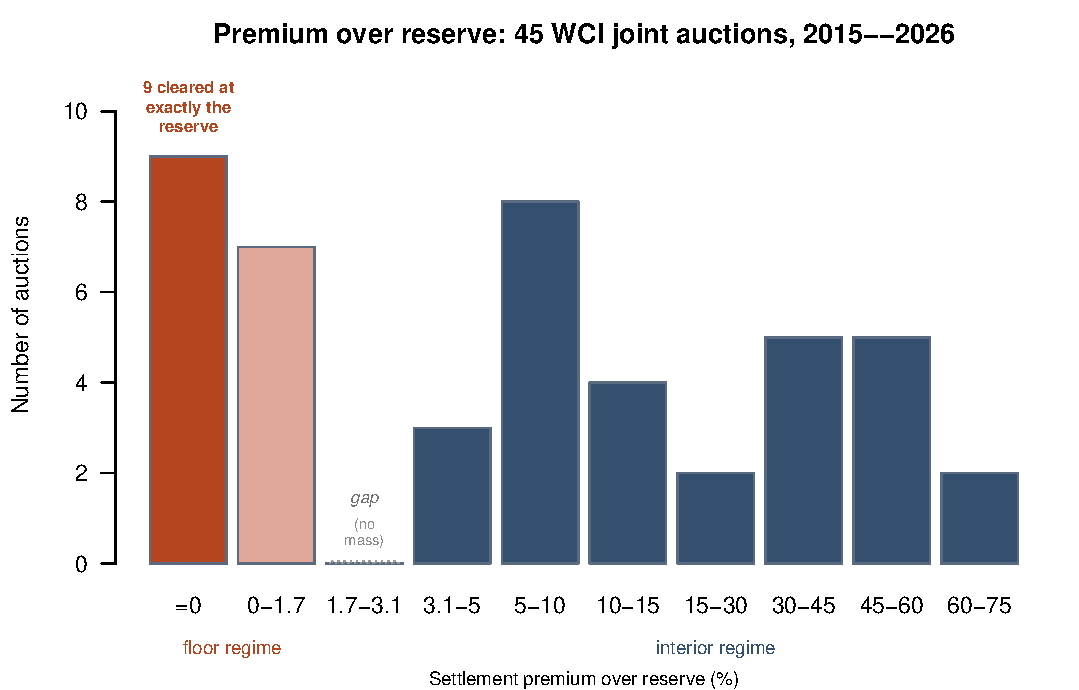
\includegraphics[width=0.78\textwidth]{figures/figure_premium.pdf}
  \caption{Settlement premium over the reserve across the 44 joint auctions, 2015Q2--2026Q1.
  Nine auctions cleared at exactly the reserve (Table~\ref{tab:reserveauctions}); a further seven settled within $1.7\%$ of it. No auction settled between $1.7\%$ and $3.5\%$; a gap of this width is unremarkable in a sample of this size (Section~\ref{sec:predictions}) and is shown as descriptive. The anchor is the mass point at exactly zero, which no continuous-settlement mechanism produces. The premium then spreads continuously to $74\%$ across the 2021--2024 interior episode.}
  \label{fig:premium}
\end{figure}

\subsection{Price-series construction and splice diagnostics}\label{app:splice}

The daily price series concatenates three instruments. Table~\ref{tab:splice} records each segment and the diagnostics at the two seams: the level gap between instruments on overlapping or adjacent dates and, where overlap exists, the correlation of daily changes.

\begin{table}[H]\centering
\caption{Price-series construction and seam diagnostics.}
\label{tab:splice}
\footnotesize
\begin{tabular}{@{}l l l l@{}}
\toprule
Segment & Instrument & Source & Range\\
\midrule
2013--2017 & Front-December futures settlement (current vintage) & California Carbon Dashboard & daily\\
2018--2020 & Current-auction settlement & CARB/WCI auction reports & quarterly\\
2021--2026 & Secondary-market settlement & ICAP & daily\\
\midrule
Seam & \multicolumn{3}{l}{Overlap diagnostic: daily instrument vs.\ auction settlement, matched auction dates}\\
\midrule
2017/18 & \multicolumn{3}{l}{gap median $+1.28$\% / change corr.\ $0.75$ ($n=11$); ex-2016--17 episode: $+1.65$\% / $0.95$ ($n=6$)}\\
2020/21 & \multicolumn{3}{l}{gap median $+4.66$\% (auction discount, see notes); change corr.\ $0.89$ ($n=20$)}\\
\bottomrule
\end{tabular}

\smallskip
{\footnotesize\justifying
\textit{Notes.}
The bridge segment is quarterly, so seam diagnostics compare the daily instrument against the current-auction settlement on matched auction dates (nearest trading day, $\pm3$ days) within each overlap window; ``change corr.''\ is the Pearson correlation of settlement-to-settlement changes. At the 2017/18 seam the five 2016--17 auctions cleared at the reserve while the daily instrument traded through it (Remark~\ref{rem:2016}); the ex-episode figures are the splice diagnostic proper. The positive gap in the 2021--26 window is the interior-regime auction discount (quarterly primary supply clears below the prevailing secondary level) and its dispersion widens when the market moves within the bid window (maximum $+15.4$\%, August 2022, in the rally preceding the AB~1279/Scoping Plan tightening; $\approx+5$\% at the May and December 2021 lift-off and purchase-limit auctions), with settlement-to-settlement changes nonetheless co-moving at $0.89$. No daily-frequency statistic in the paper crosses a splice seam: the price--volatility panel of Prediction~\ref{pred:volprice} uses the two daily segments only, and the bridge segment enters annual means and regime classification alone, for which the auction settlement is the direct observable.\par}
\end{table}

\subsection{Complementary Figures}\label{app:figs}
\begin{figure}[H]
  \centering
  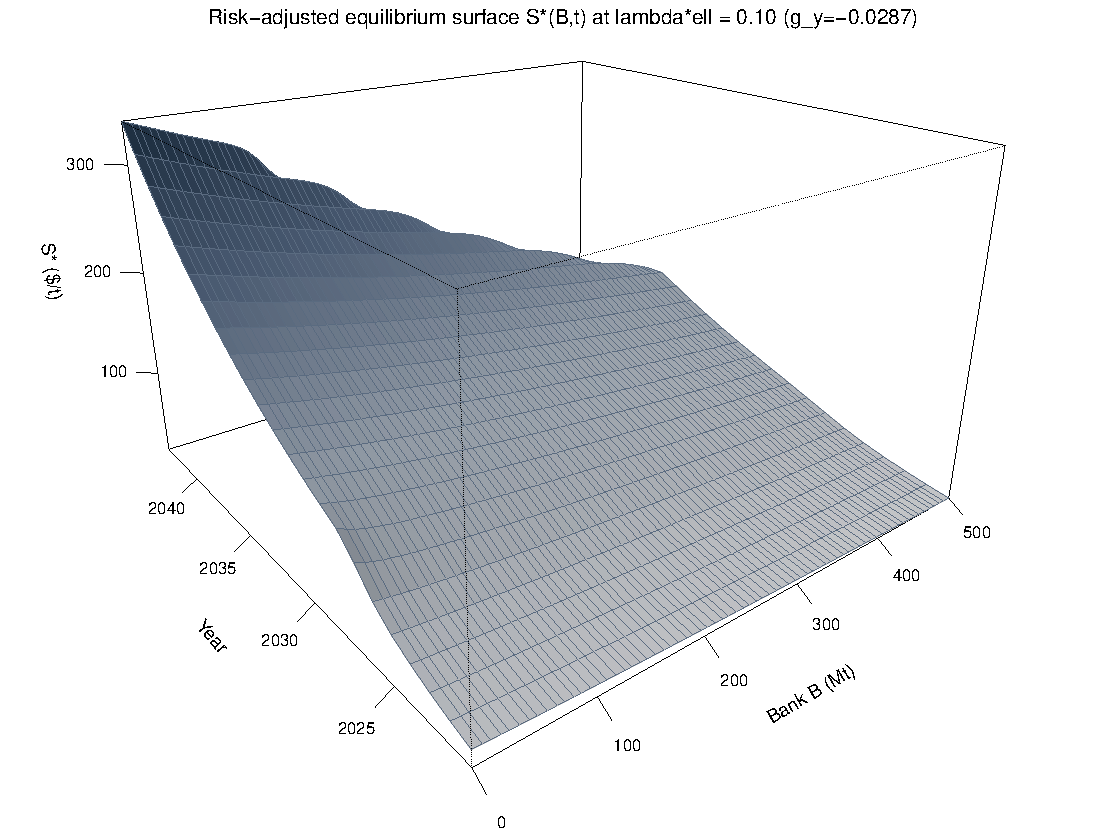
\includegraphics[width=0.85\textwidth]{figures/figure_surface.pdf}
  \caption{The equilibrium price surface $S^{\star}(B,t)$ under expected emissions, the adopted cap, and the fitted discount wedge $\lambda\ell=0.10$, on the axes of \citet{hitzemann2018}, Figure~1. Shown for completeness, the body uses the slices of Figure~\ref{fig:surface}.}
  \label{fig:surfacepersp}
\end{figure}

\begin{figure}[H]
  \centering
  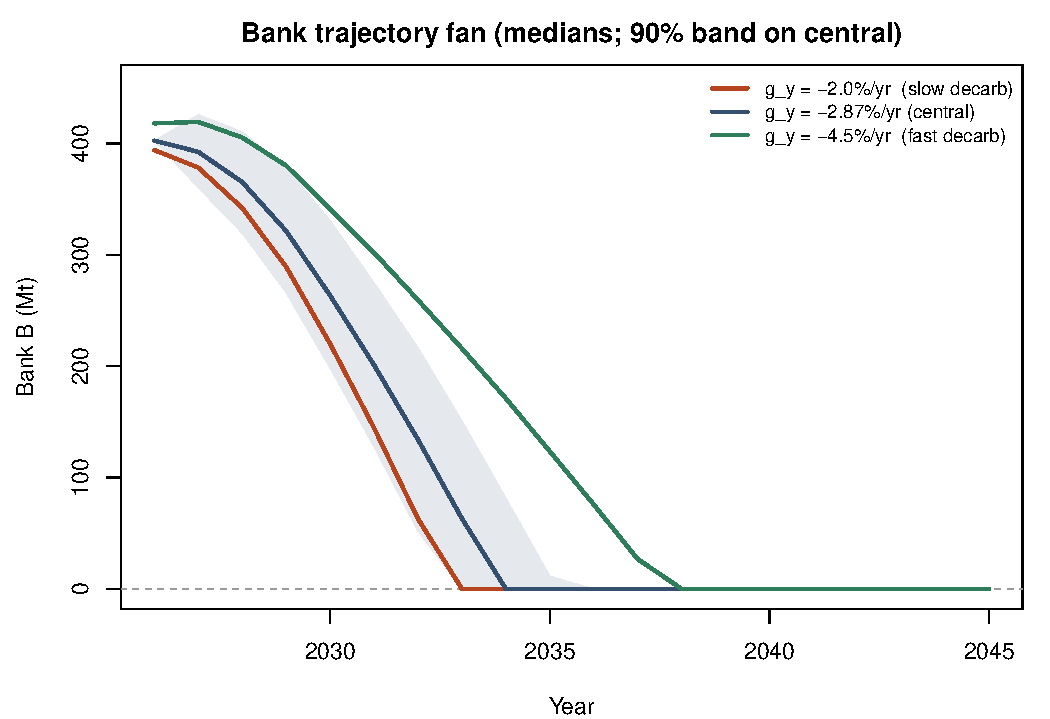
\includegraphics[width=0.80\textwidth]{figures/figure_projection_fan.pdf}
  \caption{Simulated bank trajectories under the adopted cap: scenario medians (lines) with the $90\%$ band on the central scenario (shaded), floored at zero (Regime~3 absorbing). Companion to Figure~\ref{fig:projection}.}
  \label{fig:projectionfan}
\end{figure}

\section{Numerical scheme and convergence}\label{app:numerics}
\subsection{Numerical convergence}\label{subsec:convergence}
We do not establish existence and uniqueness analytically (Section~\ref{subsec:wellposedness} sketches the result we expect); we instead verify that the finite-difference scheme of Section~\ref{sec:solver} converges and that the quantities the paper reports are stable under refinement. We refine one dimension at a time, holding the other fixed at a resolution whose time step satisfies the CFL bound $dt<\Delta B/\max|\mu_B|$ at every grid (enforced and confirmed in each run). Table~\ref{tab:convergence} reports, at each resolution, the reference interior value $S^{\mathrm{int}}(400,t_0)$, the median equilibrium price $S^{\star}$ over the 2021--2026 sample (the price level), and the change in the full $t_0$ price profile relative to the next-coarser grid in the average ($L^1$) norm.

\begin{table}[H]\centering
\caption{Convergence of the interior solver under spatial ($N_B$) and temporal ($dt$) refinement. $\|\Delta P\|$ is the change in the $t_0$ price profile versus the next-coarser grid; ``order'' is $\log_2$ of successive ratios. CFL is satisfied at every grid. $B_{\max}=800$, $\gamma=6.1$, $g_y=-2.87\%$, $\lambda\ell=0.10$, net-incremental feedback.}
\label{tab:convergence}
\footnotesize
\begin{tabular}{@{}l c c c c@{}}
\toprule
 & $S^{\mathrm{int}}(400,t_0)$ & $\mathrm{med}\,S^{\star}$ & $\|\Delta P\|_1$ & order ($L^1$)\\
\midrule
\multicolumn{5}{@{}l}{\textit{Spatial refinement, } $dt=0.0025$ \textit{ fixed}}\\
\quad $N_B=200$  & $21.6185$ & $31.9$  & ---    & ---\\
\quad $N_B=400$  & $21.6003$ & $31.9$  & $0.0158$ & ---\\
\quad $N_B=800$  & $21.5913$ & $31.9$  & $0.0078$ & $1.02$\\
\quad $N_B=1600$ & $21.5868$ & $31.9$  & $0.0038$ & $1.03$\\
\addlinespace[2pt]
\multicolumn{5}{@{}l}{\textit{Temporal refinement, } $N_B=400$ \textit{ fixed}}\\
\quad $dt=0.008$ & $21.5931$ & $31.9$  & ---    & ---\\
\quad $dt=0.004$ & $21.6053$ & $31.9$  & $0.0101$ & ---\\
\quad $dt=0.002$ & $21.6045$ & $31.9$  & $0.0009$ & ---\\
\quad $dt=0.001$ & $21.6040$ & $31.9$  & $0.0005$ & $1.00$\\
\bottomrule
\end{tabular}
\end{table}

Two features stand out. First, the reported quantities are stable to the cent: the reference interior value moves by \$0.005 from $N_B=800$ to $1600$ and by under \$0.02 across the temporal sweep, and the median price level $\mathrm{med}\,S^{\star}$ is constant at \$31.9 on every grid, within two dollars of the observed 2021--2026 median, the level fit of Section~\ref{sec:ident} read directly off the refinement table. Second, the convergence rate is first order in both dimensions ($\approx1.0$ in $L^1$; the isolated temporal ratio of $3.5$ occurs where successive differences fall to the sub-cent noise floor and carries no information). First order is the expected and correct rate for a monotone upwind scheme, and monotonicity is retained deliberately: a higher-order scheme would not preserve the comparison structure on which convergence to the viscosity solution rests \citep{barles1991}.

%==============================================================================
\bibliographystyle{plainnat}
\bibliography{references}   % expects references.bib
%==============================================================================
\end{document}
